%%%%%%%%%%%%%%%%%%%%%%%%%%%%%%%%%%%%%%%%%%%%%%%%%%%%%%%%%%%%%%%%%%%%%%%%%
%% LaTeX book template                                                 %%
%% Author:  Amber Jain (https://github.com/amberj/latex-book-template) %%
%% License: ISC license                                                %%
%%%%%%%%%%%%%%%%%%%%%%%%%%%%%%%%%%%%%%%%%%%%%%%%%%%%%%%%%%%%%%%%%%%%%%%%%

\documentclass[a4paper,11pt,oneside]{book}

\usepackage[portuguese]{babel}
\usepackage[T1]{fontenc}
\usepackage[utf8]{inputenc}
\usepackage{lmodern}
\usepackage{hyperref}
\usepackage{graphicx} % to set a images directory
\usepackage{xcolor} % changing colors
\usepackage[hang,flushmargin]{footmisc} % remove footnote's indentation
\usepackage{amsmath} % alguns símbolos matemáticos
\usepackage{float}
\usepackage{fancyvrb} % indentation in verbatim (muito bom!)
\usepackage{makecell} % multiline cell in table
% \usepackage{circuitikz} % para desenhar circuitos lógicos

\DeclareUnicodeCharacter{0301}{\'{e}}
\graphicspath{{./images/}} % set an default images folder
% \pagecolor[rgb]{0.7,0.7,0.7} % color theme no pdf
\setlength{\parindent}{0ex} % tirando indentation dos paragraphs

%%%%%%%%%%%%%%%%%%%%%%%%%%%%%%%%%%%%%%%%%%%%%%%%%%%
% First page of book which contains 'stuff' like: %
%  - Book title, subtitle                         %
%  - Book author name                             %
%%%%%%%%%%%%%%%%%%%%%%%%%%%%%%%%%%%%%%%%%%%%%%%%%%%

% Book's title and subtitle
\title{
	\Huge \textbf{Meus Estudos em Análise e Desenvolvimento de Sistemas}  \\
	\huge PUC-MG
}

% Author
\author{
	\textsc{Bruno de M. Ruas}
}

\begin{document}

\frontmatter

\maketitle

%%%%%%%%%%%%%%%%%%%%%%%%%%%%%%%%%%%%%%%%%%%%%%%%%%%%%%%%%%%%%%%%%%%%%%%%
% Auto-generated table of contents, list of figures and list of tables %
%%%%%%%%%%%%%%%%%%%%%%%%%%%%%%%%%%%%%%%%%%%%%%%%%%%%%%%%%%%%%%%%%%%%%%%%
\tableofcontents
%\listoffigures
%\listoftables

\mainmatter

%%%%%%%%%%%%%%%%%%%%%%%%%%%%%%%%%%%%%%%%%%%%%%%%%%%%%%%%%%%%%%%%%%%%%%%%
\part{Implementação de Sistemas de Software}
%%%%%%%%%%%%%%%%%%%%%%%%%%%%%%%%%%%%%%%%%%%%%%%%%%%%%%%%%%%%%%%%%%%%%%%%

%%%%%%%%%%%%%%%%%%%%%%%%%%%%%%%%%%%%%%%%%%%%%%%%%%%%%%%%%%%%%%%%%%%%%%%%
\chapter{Projeto: Desenvolvimento Web Front-End}
%%%%%%%%%%%%%%%%%%%%%%%%%%%%%%%%%%%%%%%%%%%%%%%%%%%%%%%%%%%%%%%%%%%%%%%%

\section{Etapa 1}

Objetivo da Etapa: Definir o problema a ser solucionado e os componentes do seu grupo de trabalho. Nesta etapa você entregará como tarefa dois artefatos: a \textbf{documentação de contexto} e a \textbf{especificação do projeto}.
\\~\\
O template da documentação do projeto pode ser baixado nesse \href{https://pucminas.instructure.com/courses/87866/files/5289771?wrap=1}{LINK}
\\~\\
Microfundamentos a serem estudados:
\begin{itemize}
	\item Matemática Básica
	\item Pensamento Computacional
	\item Fundamentos de Engenharia de Software
\end{itemize}

\section{Etapa 2}

Objetivo da Etapa: Projetar a interface da aplicação e a arquitetura da solução, além de definir o ambiente de trabalho que será utilizado pela equipe para desenvolver o projeto. Os artefatos a serem produzidos são: \textbf{Projeto de Interface}, \textbf{Metodologia} e \textbf{Arquitetura da Solução}.
\\~\\
Microfundamentos a serem estudados:
\begin{itemize}
	\item Fundamentos de Engenharia de Software
	\item Desenvolvimento Web Front-End
	\item Lógica Computacional
\end{itemize}

\section{Etapa 3}

Objetivo da Etapa: Desenvolver a homepage e, pelo menos, uma funcionalidade da solução projetada. O primeiro artefato a ser gerado é o \textbf{Template do site}, que determina o layout padrão do site (HTML e CSS) que será utilizado em todas as páginas com a definição de identidade visual, aspectos de responsividade e iconografia. No desenvolvimento das funcionalidades, cada artefato gerado (código fonte) deve estar relacionado a um requisito funcional e/ou não funcional.
\\~\\
Microfundamentos a serem estudados:
\begin{itemize}
	\item Desenvolvimento Web Front-End
	\item Algoritmos e Lógica de Programação
\end{itemize}

\section{Etapa 4}

Objetivo da Etapa: Finalizar o desenvolvimento da solução e irá elaborar e executar o plano de testes funcionais. Os artefatos serão: O \textbf{plano de testes de software} e O \textbf{Registro de Testes de Software}.
\\~\\
Microfundamentos a serem estudados:
\begin{itemize}
	\item Algoritmos e Lógica de Programação
	\item Fundamentos de Engenharia de Software
	\item Algoritmos e Abstração de Dados
\end{itemize}

\section{Etapa 5}

Objetivo da Etapa: Apresentar a versão final da solução implantada.
\\~\\
A apresentação do projeto consiste na geração de um conjunto de slides em um arquivo no formato ppt, pptx ou pdf, contemplando os seguintes itens:
\begin{itemize}
	\item	Contexto (Problema, Público-alvo);
	\item	Requisitos;
	\item	Solução Implementada (funcionalidades de software);
	\item	Conclusão da elaboração do projeto (pontos positivos, desafios, aprendizado).
\end{itemize}

Recomenda-se não ultrapassar 10 slides, pois o tempo de apresentação é limitado a 10 minutos, sendo 5 minutos para o projeto (slides) e 5 minutos para a demonstração da aplicação.
\\~\\
A equipe também deverá gravar um vídeo de, no máximo, três minutos, com a apresentação da solução. Vocês deverão abrir a aplicação hospedada e apresentar o seu funcionamento.
\\~\\
Microfundamentos a serem estudados:
\begin{itemize}
	\item Fundamentos de Engenharia de Software
	\item Organização de Computadores
\end{itemize}

%%%%%%%%%%%%%%%%%%%%%%%%%%%%%%%%%%%%%%%%%%%%%%%%%%%%%%%%%%%%%%%%%%%%%%%%
\chapter{Algoritmos e Abstração de Dados}
%%%%%%%%%%%%%%%%%%%%%%%%%%%%%%%%%%%%%%%%%%%%%%%%%%%%%%%%%%%%%%%%%%%%%%%%

\section{Bibliografia}

Bibliografia Básica

\begin{itemize}
	\item ASCENCIO, Ana Fernanda Gomes; CAMPOS, Edilene Aparecida Veneruchi de. Fundamentos da programação de computadores. São Paulo: Pearson, 2012. ISBN 9788564574168
	\item SOUZA, Marco A. Furlan de; GOMES, Marcelo Marques; SOARES, Marcio Vieira; CONCÍLIO, Ricardo. Algoritmos e lógica de programação: um texto introdutório para a engenharia. São Paulo: Cengage Learning, 2019. ISBN: 9788522128150
	\item ACM TRANSACTIONS ON PROGRAMMING LANGUAGES AND SYSTEMS. New York: Association for Computing Machinery.,1979-. 6 times a year. Absorvido ACM letters on programming languages and systems. ISSN 0164-0925. Disponível em: https://dl-acm-org.ez93.periodicos.capes.gov.br/citation.cfm?id=J783
	\item AGUILAR, Luis Joyanes. Fundamentos de programação algoritmos, estruturas de dados e objetos. 3. ed. Porto Alegre: AMGH, 2008. ISBN: 9788580550146
\end{itemize}

Bibliografia Complementar

\begin{itemize}
	\item DEITEL, Harvey M; DEITEL, Paul J. Java - como programar. 8. ed. São Paulo: Pearson, 2010. ISBN 9788576055631
	\item GRIFFITHS, Ian. Programming C\# 8.0. O'Reilly Media, Inc. 2019. ISBN 9781492056812
	\item MANZANO, José Augusto N. G; OLIVEIRA, Jayr Figueiredo de. Algoritmos: lógica para desenvolvimento de programação de computadores. 28. ed. rev. e atual. São Paulo, SP: Érica, 2016. E-book. ISBN 9788536518657
	\item PROGRAMMING AND COMPUTER SOFTWARE. New York, Consultants Bureau, 1975-. Bimestral. ISSN 1608-3261. Disponível em: https://link-springer-com.ez93.periodicos.capes.gov.br/ \\ journal/volumesAndIssues/11086
	\item PRICE, Mark J. C\# 8.0 and .NET Core 3.0 - Modern Cross - Platform Development. O'Reilly Media; 2019. ISBN 9781788478120
	\item PUGA, Sandra; RISSETTI, Gerson. Lógica de programação e estruturas de dados com aplicações em Java. 2. ed. São Paulo: Prentice Hall, 2009. ISBN 9788576052074
\end{itemize}

\section{Estrutura de Dados Homogêneas e Heterogêneas}
\subsection{Estrutura de Dados Homogêneas}
\subsection{Estrutura de Dados Heterogêneas}

\section{Tipos Abstratos de Dados - Classes - Implementação}
\subsection{Definição de um TAD - Classes e Objetos}
\subsection{Atributos, Propriedades e Métodos de Classe}
\subsection{Mecanismos de Visibilidade/Acessibilidade}
\subsection{Construtores de Classe}

%%%%%%%%%%%%%%%%%%%%%%%%%%%%%%%%%%%%%%%%%%%%%%%%%%%%%%%%%%%%%%%%%%%%%%%%
\chapter{Algoritmos e Lógica de Programação}
%%%%%%%%%%%%%%%%%%%%%%%%%%%%%%%%%%%%%%%%%%%%%%%%%%%%%%%%%%%%%%%%%%%%%%%%

\section{Bibliografia}

Bibliografia Básica

\begin{itemize}
	\item Ana Fernanda Gomes ASCENCIO; Edilene Aparecida Veneruchi de CAMPOS. Fundamentos da Programação de Computadores: algoritmos, Pascal, C/C++ e Java - 2ª edição. São Paulo, SP : Pearson Education do Brasil, 2012
\end{itemize}

Bibliografia Complementar

\begin{itemize}
	\item H. DEITEL et. Al.  C\#: Como Programar. São Paulo: Makron Books, 2003
	\item John SHARP. Microsoft Visual C\# 2013. Grupo A, 2014
	\item André Luiz Villar FORBELLONE, Henri Frederico EBERSPÄCHER. Lógica de programação: a construção de algoritmos e estruturas de dados. São Paulo: Prentice Hall, 2005.
	\item MANZANO, José Augusto N. G; OLIVEIRA, Jayr Figueiredo de. Algoritmos: lógica para desenvolvimento de programação de computadores 28. ed. rev. e atual. São Paulo, SP: Érica, 2016
	\item Sandra PUGA, Gerson RISSETTI. Lógica de Programação e Estrutura de Dados: com aplicações em Java - 2ª edição. São Paulo : Pearson, 2017
\end{itemize}

\section{Lógica de Programação e Estrutura de Controle, Funções e Procedimentos}

\subsection{Conceito de Algoritmo}

Em resumo, um algoritmo é uma sequência de ordens que, se seguidas, deve gerar um resultado previsto e desejado. Não vale muito a pena aprofundar além disso agora.

\subsection{Variáveis}

Uma variável é uma posição na memórida do computador. Isso mesmo, é algo com endereço definido, nada solto no universo ou obscuro dentro da máquina. Esse dado é gravado para posterior leitura por parte do programa que está sendo executado.
\\~\\
Podemos ter como origem do dado o próprio programa que está sendo executado ou o usuário por meio da entrada de dados ou, ainda, a leitura de dados previamente armazenados na memória do computador.
\\~\\
Cada variável possui vários tipos de atributos que podemos elencar na lista abaixo:
\begin{itemize}
	\item Tem um endereço na memória
	\item Possui um nome de identificação
	\item Armazena um valor
	\item Possui um tipo de dados
		\begin{itemize}
			\item Numérico - Inteiros e Reais (Double ou Ponto Flutuante)\footnote{Float possui precisão simples e Double possui dupla precisão.}
			\item Não numérico - Lógico e Caractere
			\item Arranjos - Vetores e Matrizes
			\item Arquivos
			\item etc
		\end{itemize}
\end{itemize}

O endereço da memória é feita pelos indereços que possuem apenas 2 estágios de registro: 0 ou 1. Um bit é exatamente essa medida de registo. 1 byte é composto de 8bits. 1 kilobyte contém 1024bytes ($2^{10}$). 1 megabyte contém 1024KB ($2^{20}$). 1 gigabyte contém 1024MB ($2^{30}$). 1 terabyte possui 1024GB ($2^{40}$).
\\~\\
Ou seja, se um computador possui 3 gigas de memória RAM, ele tem 3 bilhões de bytes como endereços disponíveis para um registro na memória\footnote{Isso é muito impressionante!}. Cada byte possui um endereço único. Na memória RAM costuma-se usar a base Hexadecimal para definir os endereços. Vamos ver isso melhor na matéria de Arquitetura de Computadores.
\\~\\
Também vimos que as variáveis possuem identificadores. Em c\# existem regras para a criação dos identificadores:
\begin{itemize}
	\item Devem começar com uma letra
	\item Não podem ter espaços
	\item Não podem usar uma das palavras reservadas pela linguagem
	\item É case sensitive, ou seja, o nome "Var"\ é diferente do nome "var"
\end{itemize}

O identificador deve sempre ter algum sentido que permita a rápida interpretação por parte de algum leitor do código fonte da aplicação. Isso é fundamental para manutenção de códigos produzidos por várias pessoas diferentes. Entretanto, devemos evitar nomes de variáveis muito grandes. Na verdade, quanto menor o nome, mantido o sentido na leitura, melhor.
\\~\\
Outra boa prática é usar o camelCase para variáveis com mais de uma palavra. Esse padrão é bem simples: primeira palavra em minúsculo e a segunda com a primeira letra em maiúscula.
\\~\\
\textbf{Declaração de Variáveis em c\#}
\\~\\
Vamos aprender agora como declarar os 4 tipos mais simples de variáveis:
\begin{itemize}
	\item \verb|int| para definir inteiros
	\item \verb|double| ou \verb|float| para definir números reais
	\item \verb|string| para cadeia de caracteres
	\item \verb|bool| para as variáveis booleanas (\verb|true| ou \verb|false|)
\end{itemize}

\begin{center}
\begin{Verbatim}[tabsize=4,frame=single]
static void Main(string[] args) 
{
	int idade, numero;
	double peso, salario;
	string nomePai, rua, dtNasc;
	bol temCasa;
} 
\end{Verbatim}
\end{center}

Nesse código acima temos a declaração de várias variáveis de cada tipo. Basta colocar o tipo da variável seguido do nome de cada uma delas separadas por vírgula.
\\~\\
\textbf{Comentário:} Em c\# todas as linhas precisam conter um caracter de encerramendo que é o ponto e vírgula \verb|;|. Sem esse token, o computador vai interpretar a próxima linha como sendo a continuação da anterior.

\subsection{Etapas de um Algotimo e Operador de Atribuição}

Podemos resumir um algotimo simples como contendo apenas 3 etapas: 1) A entrada de dados; 2) O processamento e 3) A saída de dados.
\\~\\
Na etapa de processamento, podemos precisar de grande criatividade e esforço para produzir a saída de dados desejada. Como ferramenta para alcance desse objetivo, temos as \textbf{estruturas básicas} que são:
\begin{itemize}
	\item Estrutura Sequencial - Usada para garantir a ordem correta dos passos
	\item Estrutura Condicional - Usada para permitir contexto ou cenários 
	\item Estrutura de Repetição - Usada para evitar repetir código sequencial
\end{itemize}

\subsubsection{Operador de Atribuição}

Uma vez que já sabemos como atribuir uma variável ao seu tipo, precisamos aprender a como atribuir um valor a essas variáveis. Em c\# a atribuição de valor é feita do seguinte modo:

\begin{center}
\begin{Verbatim}[tabsize=4,frame=single]
idade = 28;
numero = 9992233;
\end{Verbatim}
\end{center}

É possível fazer 3 tipos de atribuição de valor para uma variável: Valor fixo; Conteúdo de outra variável e Expressão aritmética ou booleana. Abaixo temos 3 exemplo disso.

\begin{center}
\begin{Verbatim}[tabsize=4,frame=single]
idade = 28; // Valor fixo
numero = idade; // Valor de outra variavel
idadeNum = idade + numero; // Valor por expressão
idadeEqNum = idade == numero; // Valor por expressao booleana
\end{Verbatim}
\end{center}

Nesse ponto vale uma reflexão. Será que sempre precisamos separar as etapas de atribuição do tipo de dados e do valor? Ou podemos, no mesmo momento, definir o tipo de dados e o valor da variável? A resposta, para nossa sorte, é que é possível em c\# atribuição de tipo e valor ao mesmo tempo. A sintaxe fica desse modo:

\begin{center}
\begin{Verbatim}[tabsize=4,frame=single]
int idade = 28;
int numero = idade;
double = 2.3;
string nome = "bruno";
int idadeNum = idade + numero;
bool idadeEqNum = idade == numero;
\end{Verbatim}
\end{center}

\textbf{Saída de Dados}
\\~\\
Agora que fizemos esse pequeno desvio no assunto, vamos retornar para as estruturas. Por incrível que pareça, é melhor a gente começar pelo final. A etapa de saída de dados.
\\~\\
Em c\# temos duas maneiras de saída de dados:

\begin{center}
\begin{Verbatim}[tabsize=4,frame=single]
// Imprime a informacao e cursor fica na mesma linha
Console.Write('string');

// Imprime a info mas o curso vai pra proxima linha
Console.WriteLine('string ' + var1 + ' string');
\end{Verbatim}
\end{center}

Nesses exemplos a gente pode perceber que podemos concatenar textos e variáveis textuais por meio do operador de soma. Além dessa forma, podemos fazer uso de PlaceHolders ou Interpolação de string como nos exemplos abaixo.

\begin{center}
\begin{Verbatim}[tabsize=4,frame=single]
string nome = "Bruno";

// Concatenacao
Console.WriteLine("Meu nome é " + nome + ", obrigado!");

// PlaceHolder
Console.WriteLine("Meu nome é {0}, obrigado!", nome);

// Interpolacao
Console.WriteLine($"Meu nome é {nome}, obrigado!");
\end{Verbatim}
\end{center}

Os três exemplos geram o mesmo restulado mas são consideravelmente diferentes no método. Podemos usar o que for mais agradável para uma leitura do código e posterior manutenção do mesmo.
\\~\\
\textbf{Entrada de Dados}
\\~\\
Agora que sabemos como fazer nosso programa imprimir resultados, vamos aprender como inputar dados nele. Em c\# podemos inserir dados com o seguinte comando:

\begin{center}
\begin{Verbatim}[tabsize=4,frame=single]
variavel = Console.ReadLine();
\end{Verbatim}
\end{center}

O input captado por esse comando \textbf{sempre retorna uma string}. Mas as vezes precisamos nos certificar que o input foi feito da maneira correta. Para isso podemos manipular os dados inseridos do seguite modo:

\begin{center}
\begin{Verbatim}[tabsize=4,frame=single]
// Valores Inteiros
variavel = int.Parse(Console.ReaLine());
variavel = Convert.ToInt32(Console.ReadLine());

// Valores Reais
variavel = double.Parse(Console.ReadLine());
variavel = float.Parse(Console.ReadLine());
variavel = Convert.ToDouble(Console.ReadLine());

// Valores Booleanos
variavel = bool.Parse(Console.ReadLine());

// Valores String
variavel = Console.ReadLine();
\end{Verbatim}
\end{center}

Depois que executamos um dessas maneiras de coletar os dados, é de boa prática fornecermos um output logo após a entrada do dado. Isso evita aquela sensação de dúvida se o programa está sendo executado ou não. Ou seja, é bom sempre manter a dupla \verb|ReadLine()| com o \verb|WriteLine()|. O nome que damos para essa dupla é "Prompt".
\\~\\
Outra dica boa é usar o comando \verb|Console.ReadKey()| no final do programa. Isso faz com que o console aguarde alguma tecla para finalizar. Evita que a aplicação abra e feche sem que o user consiga enxergar o resultado do processo.

\subsection{Estrutura Sequencial}

Agora que sabemos como receber valores do usuário e como devolver nova informação a partir do processamento, vamos começar a estudar a etapa de processamento através do estudo das estruturas sequenciais.

\subsubsection{Operadores e Funções Aritméticas}

Em c\# nós temos os seguintes tokens para realizar as operações aritiméticas:
\begin{itemize}
	\item \verb|+| Soma
	\item \verb|-| Subtração
	\item \verb|*| Multiplicação
	\item \verb|/| Divisão
	\item \verb|%| Resto da Divisão inteira
\end{itemize}

Além disso, temos a presença do que podemos chamar de \textbf{operadores de atribuição combinada}. Que faz a atribuição de valor com alguma operação aritimética:
\begin{itemize}
	\item soma += 100 é igual a soma = soma + 100
	\item subtracao -= 10 é igual a subtracao = subtracao - 10 
	\item multiplica *= 2 é igual a multiplca = multiplca * 2
	\item divide /= 3 é igual a divide = divide / 3
	\item resto \%= 2 é igual a resto = resto / 2
\end{itemize}

Não bastando essa grande variedade, temos os operadores de \textbf{incremento e decremento}:
\begin{itemize}
	\item Pré-incremento (\verb|++x|) - Usa x + 1 antes do processamento
	\item Pós-incremento (\verb|x++|) - Usa x + 1 após o processamento
	\item Pré-decréscimo (\verb|--x|) - Usa x - 1 antes do processamento
	\item Pós-decréscimo (\verb|x--|) - Usa x -1 após o processamento
\end{itemize}

Essa diferença de pre e pós é importante para as estruturas de repetição, porque podemos lidar com índices de tabelas que começam com valores diferentes. Mas, no geral, devemos olhar cada caso para escolher o que usar.
\\~\\
Existem outras operações que estão contidas em um objeto nativo chamado \verb|Math|. Para fazermos potenciação usamos o método \verb|Math.Pow()|. Para fazermos raiz quadrada podemos usar \verb|Math.Sqrt()|\footnote{Embora a gente saiba que a radiciação é uma potência de fração.}.


\subsubsection{Expressões Aritméticas}

Agora podemos juntar tudo que vimos em um programa simples de cálculo da média de 5 valores. O código e o seu resultado podem ser vistos abaixo.

\scriptsize
\begin{center}
\begin{Verbatim}[tabsize=4,frame=single]
// Declaracao dos tipos das variaveis
int n1, n2, n3, n4, n5, soma;
float media;

// Input dos dados
Console.WriteLine("Programa para cálculo da média de 5 valores.");

Console.WriteLine("Por favor, forneça o primeiro número");
n1 = Convert.ToInt32(Console.ReadLine());
Console.WriteLine("Por favor, forneça o segundo número");
n2 = Convert.ToInt32(Console.ReadLine());
Console.WriteLine("Por favor, forneça o terceiro número");
n3 = Convert.ToInt32(Console.ReadLine());
Console.WriteLine("Por favor, forneça o quarto número");
n4 = Convert.ToInt32(Console.ReadLine());
Console.WriteLine("Por favor, forneça o quinto número");
n5 = Convert.ToInt32(Console.ReadLine());

// Processamento
soma = n1 + n2 + n3 + n4 + n5;
media = soma / 5;

// Output dos dados
Console.WriteLine("Os números fornecidos foram:");
Console.WriteLine("N1={0},N2={1},N3={2},N4={3},N5={4}", n1, n2, n3, n4, n5);
Console.WriteLine("Cuja média é igual a {0}", media);
\end{Verbatim}
\end{center}
\normalsize

\begin{figure}[H]
	\centering
	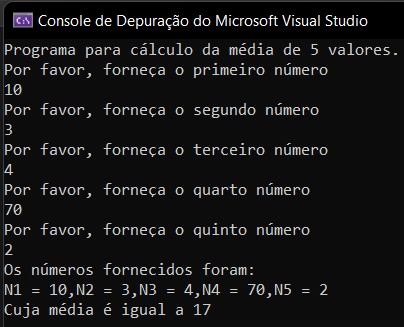
\includegraphics[scale=0.8]{25-algoritmo-logica-media-cs.png}
	\caption{Programa de cálculo da média de 5 valores em c\#}
\end{figure}

Outro exemplo que podemos usar é o do cálculo das raízes de uma função de segundo grau\footnote{Se você não se lembra como resolver um problema desse, seu professor da sexta série está rindo de você nesse exato minuto.}. O programa abaixo recebe 3 valores e calcula as raízes, a imagem logo após nos mostra o resultado no prompt de comando.

\scriptsize
\begin{center}
\begin{Verbatim}[tabsize=4,frame=single]
// Programa para calcular o valor de x em uma equacao de segundo grau

// Declaracao das variaveis
double a, b, c, x1, x2;

Console.WriteLine("Vamos resolver uma equação do tipo ax^2 + bx + c = 0");

// Input das variaveis
Console.WriteLine("Qual o valor de a? ");
a = Convert.ToDouble(Console.ReadLine());

Console.WriteLine("Qual o valor de b? ");
b = Convert.ToDouble(Console.ReadLine());

Console.WriteLine("Qual o valor de c? ");
c = Convert.ToDouble(Console.ReadLine());


x1 = (-b + Math.Sqrt(Math.Pow(b,2) - 4 * a * c)) / 2 * a;
x2 = (-b - Math.Sqrt(Math.Pow(b, 2) - 4 * a * c)) / 2 * a;

// Output dos resultados
Console.WriteLine("Dados: a = {0}, b = {1} e c = {2}", a, b, c);
Console.WriteLine($"Equação: (-({b}) +- Raiz(({b})^2 - 4*{a}*{c}))/2*{a} = 0");
Console.WriteLine("Resultado: x1 = {0} e x2 = {1}", x1, x2);
\end{Verbatim}
\end{center}
\normalsize

\begin{figure}[H]
	\centering
	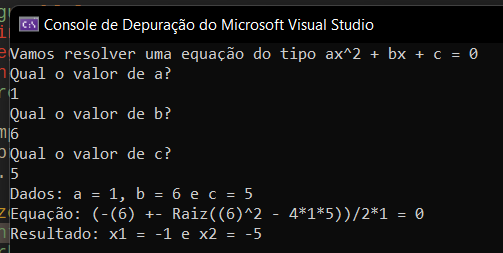
\includegraphics[scale=0.8]{26-algoritmo-equacao-grau2.png}
	\caption{Programa de resolução de uma equação do segundo grau.}
\end{figure}

A essa altura já aprendemos como criar programas inteiros com as etapas de software que vimos anterioremente: input, processamento e output. Tudo isso em c\#. Entretanto, no estado atual do código, nossos programas não estão muito competentes em se adaptar a diferentes tipos de inputs ou resultados.
\\~\\
Um exemplo prático é que, nesse segundo programa, podemos ter inputs que retornem um resultado indesejado como podemos ver na imagem abaixo.

\begin{figure}[H]
	\centering
	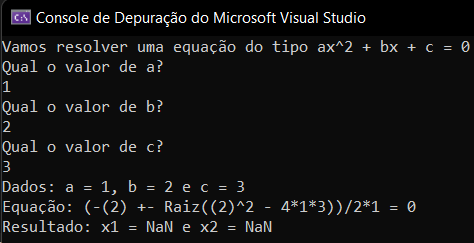
\includegraphics[scale=0.8]{27-erro-eq-grau2.png}
	\caption{Programa de resolução de uma equação do segundo grau com erro.}
\end{figure}

\subsection{Estrutura Condicional}

A necessidade de lidarmos com diferentes situações ou contextos é o que nos leva a estudarmos as \textbf{estruturas condicionais}. Por meio dessas estruturas, podemos construir diferentes outputs de acordo com qualquer lógica que implementarmos e, com isso, evitar vários bugs nos nossos programas.

\subsubsection{Operadores Relacionais}

Ao lidarmos com estrutura condicionais nós temos alguns operadores que nada mais são doque expressões lógicas que retornam apenas 2 resultados possívies: true ou false. Esses operadores são como "gatilhos"\ que são usados para controle do fluxo de processamento do código.

\begin{center}
\begin{tabular}{|c|c|c|}
\hline
\textbf{Operador} & \textbf{Operação} & \textbf{Exemplo} \\
\hline
\hline
\verb|==| & Igualdade & n1 == n2 \\
\hline
\verb|<| & Menor & a < 10 \\
\hline
\verb|>| & Maio & b > 1 \\
\hline
\verb|<=| & Menor igual & c <= 2 \\
\hline
\verb|>=| & Maior igual & d >= 22 \\
\hline
\verb|!=| & Desigualdade & e != 100 \\
\hline
\end{tabular}
\end{center}

Na tabela acima, temos os operadores relacionais que são usados ao longo das estruturas condicionais simples e compostas.
\\~\\
Tome cuidado com o operador de igualdade \verb|==| e o de atribuição \verb|=|, afinal, eles usam o sinal de igualdade mas significam coisas diferentes.

\subsubsection{Condição Simples e Composta}

Em c\# o comando usado para criar uma condição simples é o \verb|if|. Se a condição que colocarmos atrelada ao comando \verb|if| retornar um true, o bloco de código atribuído a ele será executar, caso contrário, o código do bloco será ignorado.

\scriptsize
\begin{center}
\begin{Verbatim}[tabsize=4,frame=single]
// Parte condicional no calculo da equacao de segundo grau

delta = (Math.Pow(b, 2) - 4 * a * c);

// Output dos resultados com condicao
if (delta >= 0)
{
    Console.WriteLine("Dados: a = {0}, b = {1} e c = {2}", a, b, c);
    Console.WriteLine($"Equação: (-({b}) +- Raiz(({b})^2 - 4*{a}*{c}))/2*{a} = 0");
    Console.WriteLine($"Delta: {delta}");
    Console.WriteLine("Resultado: x1 = {0} e x2 = {1}", x1, x2);
};

if (delta < 0)
{
    Console.WriteLine("Dados: a = {0}, b = {1} e c = {2}", a, b, c);
    Console.WriteLine($"Equação: (-({b}) +- Raiz(({b})^2 - 4*{a}*{c}))/2*{a} = 0");
    Console.WriteLine($"Delta: {delta}");
    Console.WriteLine("Resultado: X não possui raiz real! ");
};
\end{Verbatim}
\end{center}
\normalsize

Com essa adaptação, nosso código estará preparado para o caso onde o interior da raiz (que chamamos de delta) seja negativo. Mas podemos ver que o nosso código ficou um pouco esquisito. Criamos dois blocos de código que são, claramente, relacionados entre si: Se um bloco for executado, o outro não será. Para facilitar o trabalho com essas situações, as linguagens de programação possuem as estruturas de condição compostas.
\\~\\
Esses são os casos onde, se o teste lógico retorna true, executamos um bloco, ou o outro bloco será executado caso o resultado lógico seja false. Com isso evitamos ter que criar dois testes com \verb|if|. O token usado em c\# para uma condição com dois blocos de códigos (ou seja, uma condicional compsota) é o \verb|if-else|. Abaixo nós reescrevemos a solução anterior mas agora fazendo uso do condional composto.

\scriptsize
\begin{center}
\begin{Verbatim}[tabsize=4,frame=single]
// Parte condicional no calculo da equacao de segundo grau

delta = (Math.Pow(b, 2) - 4 * a * c);

// Output dos resultados com condicao
if (delta >= 0)
{
    Console.WriteLine("Dados: a = {0}, b = {1} e c = {2}", a, b, c);
    Console.WriteLine($"Equação: (-({b}) +- Raiz(({b})^2 - 4*{a}*{c}))/2*{a} = 0");
    Console.WriteLine($"Delta: {delta}");
    Console.WriteLine("Resultado: x1 = {0} e x2 = {1}", x1, x2);
} else
{
    Console.WriteLine("Dados: a = {0}, b = {1} e c = {2}", a, b, c);
    Console.WriteLine($"Equação: (-({b}) +- Raiz(({b})^2 - 4*{a}*{c}))/2*{a} = 0");
    Console.WriteLine($"Delta: {delta}");
    Console.WriteLine("Resultado: X não possui raiz real! ");
};
\end{Verbatim}
\end{center}
\normalsize

Agora sim nosso código está elegante e adaptado para as duas saídas possíveis de resultado para os inputs do usuário.

\subsubsection{Operadores Booleanos e Comandos IF Aninhados}

Nós aprendemos que o bloco de código será executado sempre que a expressão lógica retornar um resultado true. Também vimos que existem os operadores relacionais que nos ajudam a construir essas expressões. Agora, vamos aprender os operadores booleanos que nada mais são do que os operadores lógicos clássicos ($\land, \lor, \neg$).

\begin{center}
\begin{tabular}{|c|l|c|}
\hline
\textbf{Operador} & \textbf{Operação} & \textbf{Exemplo} \\
\hline
\hline
\verb|&& (AND)| & true se tudo for true & \verb|if (a > 2 && b == 1)| \\
\hline
\verb@|| (OR)@ & true se um for true & \verb@if (a < 2 || b != 0)@ \\
\hline
\verb|! (NOT)| & false se true & \verb|if (!(x==y))| \\
\hline
\end{tabular}
\end{center}

Existem problemas que requerem mais de dois resultados no output. Nesse caso, não é suficiente usarmos apenas os tokens de condicional composto \verb|if-else| da maneira como aprendemos até agora.
\\~\\
Para resolver esse problema temos a técnica de \verb|IF| aninhados (nested) e a de \verb|IF| escada (ladder). As duas formas produzem o mesmo resultado mas mudam significativamente legibilidade do nosso código. Abaixo temos um exemplo de cada.

\begin{center}
\begin{Verbatim}[tabsize=4,frame=single]
// Leadder IF

if (condicao1)
	comando1;
else if (condicao2)
	comando2;
else if (condicao3)
	comando3;
...
else if (condicao_n-1)
	comando_n-1;
else
	comando_n;
\end{Verbatim}
\end{center}

\begin{center}
\begin{Verbatim}[tabsize=4,frame=single]
// Nested IF

if (condicao1)
	comando1;
else
	if (condicao2)
		comando2;
	else
		if (condicao3)
			comando3;
		else
			if (condicao4)
				comando4;
		...
			else
				if (condicao_n-1)
					comando_n-1;
				else
					comando_n;
\end{Verbatim}
\end{center}

\subsubsection{O Comando Switch e o Operador Ternário}

Agora que aprendemos a lidar com vários casos condicionais encadeados, podemos construir soluções relativamente complexas com várias saídas diferentes. Entretanto, quando tempos muitas situações possíveis, o nosso código pode ficar um pouco ruim de ser lido por outras pessoas.
\\~\\
Pensando nessa necessidade, os criadores do c\# criaram um operador que simplifica ainda mais nosso trabalho. Sim, é isso mesmo, nós acabamos de aprender IFs aninhados e em escada e já vamos aprender uma maneira melhor de fazer exatamente o que eles fazem. Se acostume com isso. Em tecnologia existem quase sempre várias maneiras de se chegar no mesmo resultado.
\\~\\
O operador que é mais indicado para lidar com várias situações de saída é o \verb|swith-case|. Cuja construção é bem mais legível que os IFs anteriores. Abaixo temos um exemplo.

\begin{center}
\begin{Verbatim}[tabsize=4,frame=single]
// Lidando com varias condicoes com swith/case

swith(opcao)
{
	case op1:
		comandos1;
		break;
	case op2:
		comandos2;
		break;
	case op3:
		comandos3;
		break;
	...
	case op_n:
		comandos_n;
		break;
	default:
		bloco que sera executado se nenhuma 
		das anteriores for escolhida;
}
\end{Verbatim}
\end{center}

\textbf{Comentário:} Existem várias maneiras de se usar o switch. Eu não vou me aprofundar agora em todas elas. Mas vale muito a pena fazer uso dessa ferramenta para cenários de várias interações possíveis ou múltiplas saídas contextuais.

Para finalizar o nosso estudo das estruturas condicionais, vamos aprender como trabalhar com o \textbf{Operador ternário}. Esse nome é relativo ao número de operandos que esse comando usa (no caso, 3).

\begin{Verbatim}[tabsize=4,frame=single]
condicao ? expressao_true : expressao_false
\end{Verbatim}

A condição é uma expressão lógica (que usa operadores relacionais e booleanos) que só pode retornar true ou false. A expressão logo após o ponto de interrogação será o retorno do operador em caso de true. A expressão após os dois pontos é o retorno em caso de false.
\\~\\
Sim, é exatamente um caso de \verb|if-else| só que em apenas uma linha. Como as soluções podem ficar muito grandes, é sempre bom termos em mente que quanto menos linhas, mais fácil será fazer manutenção nos nossos programas. O operador ternário é muito usado por programadores mais experientes. Abaixo temos um exemplo comparando as duas maneiras.

\begin{Verbatim}[tabsize=4,frame=single]
// Comparacao entre if-else e operador ternario

bool passou;
double nota;

// if-else
if (nota >= 60)
	passou = true;
else
	passou = false;

// operador ternario
passou = nota >= 60 ? true : false // maneira 1
passou = (nota >= 60) ? true : false // maneira 2
\end{Verbatim}

Agora podemos ver claramente a vantagem do uso do operador ternário.

\section{Estrutura de Repetição}

Como sabemos, ainda temos mais um tipo de estrutura para estudarmos. Até agora, aprendemos como estruturar um código sequencialmente e como criar blocos de código que só serão executados se determinadas condições previamente definidas forem satisfeitas. Agora, vamos aprender como evitar ter que repetir blocos de códigos.
\\~\\
O c\# possui 3 operadores de repetição:
\begin{Verbatim}[tabsize=4,frame=single]
// tipo 01
while (condicao)
	comando;

// tipo 02
do
	comando;
while (condicao);

// tipo 03
for (inicial; inicial; atualizacao)
	comando;
\end{Verbatim}

Vamos ver um exemplo de como nosso código pode ser reduzir com o uso da estrutura de repetição. Primeiro, vamos ver um exemplo onde o programa recebe uma lista de 3 palavras (nome, nome do meio e sobrenome) e depois faz o print.

\begin{Verbatim}[tabsize=4,frame=single]
// Programa que recebe nome completo e
// depois devolve uma mensagem de boas vindas

string nome, mid, last;

Console.WriteLine(" Seja bem vindo(a)!");

Console.WriteLine(" Qual seu primeiro nome?");
nome = Console.ReadLine();

Console.WriteLine(" Qual seu nome do meio?");
mid = Console.ReadLine();

Console.WriteLine(" Qual seu sobrenome?");
last = Console.ReadLine();

Console.WriteLine(" Bem Vindo(a)!");

Console.WriteLine(nome);
Console.WriteLine(mid);
Console.WriteLine(last);

Console.WriteLine(" E Vide panel"lte sempre!");
\end{Verbatim}

\begin{figure}[H]
	\centering
	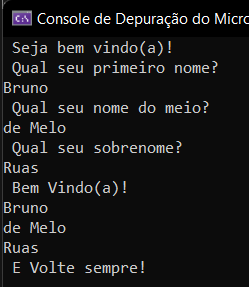
\includegraphics[scale=0.8]{28-programa-nome1.png}
	\caption{Programa simples }
\end{figure}

Agora vamos refazer esse programa usando os 3 tokens de estrutura de repetição que o c\# nos dá. Vamos usar a mesma ordem em que elas foram apresentadas.

\subsubsection{Os Comandos WHILE, DO WHILE e FOR}

\textbf{Repetição usando WHILE}
\\~\\
A repetição usando o token \verb|while| é condicionada ao resultado de uma expressão lógica. Caso a expressão lógica retorne true, o bloco de código será executado até o seu final. Após a execução, é feita uma nova verificação da expressão lógica. O processo de loop só será finalizado caso a expressão lógica retorne o valor false. Abaixo temos a refatoração\footnote{Refatorar é o processo de mudar o código e obter o mesmo resultado no final. É uma ótima prática a ser feita.} evitando a repetição de partes de partes do código anterior.

\begin{Verbatim}[tabsize=4,frame=single]
// Programa de nomes refatorado com while

string nome, mid, last;
int contador;

// nome default
nome = "";
mid = "";
last = "";

Console.WriteLine(" Seja bem vindo(a)!");

Console.WriteLine(" Por favor, insira o seu nome completo.");
Console.WriteLine(" Obs. No máximo 3 palavras");
contador = 1;

while (contador <= 3)
{   
    Console.WriteLine($" Palavra nº {contador} do seu nome?");
    if (contador == 1)
        nome = Console.ReadLine();
    else if (contador == 2)
        mid = Console.ReadLine();
    else if (contador == 3)
        last = Console.ReadLine();

    contador += 1;
};

Console.WriteLine(" Bem Vindo(a)!");
Console.WriteLine(nome);
Console.WriteLine(mid);
Console.WriteLine(last);
Console.WriteLine(" E Volte sempre!");
\end{Verbatim}

Agora nós temos um loop usando a expressão "a variável contador é menor igual a 3?"\ sempre que a resposta for sim, o programa perguntará qual a n-ésima palavra do nome da pessoa. Pode parecer que nesse exemplo o uso do loop mais complicou do que facilitou. Mas o objetivo aqui é exercitar o uso desse operador, então devemos focar em compreender como usar o while.
\\~\\
\textbf{Repetição usando DO WHILE}
\\~\\
Para a nossa sorte, o operador DO WHILE é muito similar ao WHILE. A única diferença é que primeiro declaramos o bloco de código e, no final, colocamos a condição para sua execução. No exemplo abaixo temos o mesmo resultado que o de cima mas usando essa outra estrutura de operador.

\begin{Verbatim}[tabsize=1,frame=single]
// Programa de nomes refatorado com do-while

string nome, mid, last;
int contador;

// nome default
nome = "";
mid = "";
last = "";

Console.WriteLine(" Seja bem vindo(a)!");

Console.WriteLine(" Por favor, insira o seu nome completo.");
Console.WriteLine(" Obs. No máximo 3 palavras");
contador = 1;

do
{   
  Console.WriteLine($" Palavra nº {contador} do seu nome?");
   if (contador == 1)
       nome = Console.ReadLine();
   else if (contador == 2)
       mid = Console.ReadLine();
   else if (contador == 3)
       last = Console.ReadLine();

   contador += 1;
} while (contador <= 3);

Console.WriteLine(" Bem Vindo(a)!");
Console.WriteLine(nome);
Console.WriteLine(mid);
Console.WriteLine(last);
Console.WriteLine(" E Volte sempre!");
\end{Verbatim}


\textbf{Repetição usando FOR}

\subsubsection{Contadores e Acumuladores}

\section{Manipulação de Dados em Memória Primária e Secundária}
\subsection{Criando e Usando Funções e Procedimentos}
\subsection{Passagem de Parâmetros}
\subsection{Manipulação de Arquivos em C\#}

%%%%%%%%%%%%%%%%%%%%%%%%%%%%%%%%%%%%%%%%%%%%%%%%%%%%%%%%%%%%%%%%%%%%%%%%
\chapter{Desenvolvimento Web Front-End}
%%%%%%%%%%%%%%%%%%%%%%%%%%%%%%%%%%%%%%%%%%%%%%%%%%%%%%%%%%%%%%%%%%%%%%%%

\section{Bibliografia}

Bibliografia Básica

\begin{itemize}
	\item SIKOS, L. Web Standards. Mastering HTML5, CSS3, and XML.
	\item DACONTA, M. C.; SMITH, K. T.; OBRST, L. J. The semantic Web: a guide to the future of XML, Web services, and knowledge management. [s. l.]: Wiley, [s. d.]. ISBN 0471432571
	\item SILVA, Maurício Samy. HTML 5: a linguagem de marcação quer revolucionar a web. 2. ed. rev. e ampl. [s. l.]: Novatec, 2014. ISBN 9788575224038
	\item SANDERS, William B. Smashing HTML5: técnicas para a nova geração da web. Porto Alegre: Bookman, 2012. xiv, 354 p. ISBN 9788577809608
	\item DEITEL, Paul J., Deitel, Harvey M. Ajax, Rich. Internet Applications e Desenvolvimento Web para Programadores. Pearson 776. ISBN 9788576051619
	\item SILVA, Maurício Samy. CSS3: desenvolva aplicações web profissionais com uso dos poderosos recursos de estilização das CSS3. São Paulo: Novatec, 2011. 494 p. ISBN 9788575222898
	\item BERTAGNOLLI, S. de C.; MILETTO, E. M. Desenvolvimento de software II: introdução ao desenvolvimento web com HTML, CSS, JavaScript e PHP. [s. l.]: Bookman, 2014. ISBN 9788582601952
\end{itemize}

\section{A Web: Evolução, Padrões e Arquitetura}
\subsection{Histórico e Evolução da Web}

A Web é um sistema da informação de hipertextos onde o acesso é feito por meio de \textbf{navegadores (browsers)}.
\\~\\
Existem alguns protocolos comuns para transferência de alguns tipos de arquivos. Para mensagens (e-mail) usamos o \textbf{SMTP}, para transferência de arquivos usamos o \textbf{FTP}, aplicações de telefonia usam o \textbf{VOIP} e para páginas de conteúdo usamos o \textbf{HTML}.
\\~\\
A história da web eu ainda vou colocar aqui quando tiver mais tempo.

\subsection{W3C e os Padrões da Web}

O WORLD WIDE WEB CONSORTIUM (W3C) é uma organização sem fins lucrativos cujo líder é o Tim Berners-Lee, justamente o inventor da Web. Existem várias organizações ao longo do planeta que fazem parte desse consórcio internacional.

O W3C mantém a gestão de vários padrões usados todos os dias:
\begin{itemize}
	\item Design e Aplicações Web (HTML, CSS, SVG, Ajax, Acessibilidade);
	\item Arquitetura da Web (Protocolo HTTP, URI);
	\item Web Semântica (Linked Data - RDF, OWL, SPARQL);
	\item Web Services (SOAP, WSDL);
	\item Tecnologia XML (XML, XML Schema, XSLT);
	\item Navegadores e ferramentas de autoria.
\end{itemize}

A W3C possui um processo de publicação das normativas. Normalmente, o fluxo é:
\begin{itemize}
	\item Working Draft (WD)
	\item Candidate Release (CR)
	\item Proposed Recomendation (PR)
	\item Recomendation (REC)
\end{itemize}

\subsection{Componentes da Arquitetura da Web}

A web pode ser entendida como uma coleção de componentes que permitem a comunicação entre o cliente e os servidores de aplicações. Os principais componentes dessa arquitetura são:
\begin{itemize}
	\item Ambiente Cliente (Client Web) \\~\\
			Geralmente um Browser que envia as requisições usando o protocolo HTTP(S) para o servidor web através de uma rede de computadores.
	\item Ambiente Servidor \\~\\
			O ambiente servidor possui vários componentes (banco de dados, aplicações, API e etc) mas o principal componente é o servidor web. Ele recebe a requisição HTTP(S) do client, interpreta a URL e envia os recursos solicitados (HTML, CSS, JS, JPEG, MP4 e etc) por meio da rede. 
	\item Internet \\~\\
			É a rede mundial baseada no protocolo TCP/IP onde todo computador conectado é denominado host (hospedeiro) e possui um identificador de endereço IP (internet protocol) que possui determinados padrões.
	\item URI (uniform resource locator) \\~\\
			Como o nome indica, um URI é um localizado que pode ser classificado em duas maneiras. O URL é o tipo de URI que usa o endereço do conteúdo como método de localização, ele nos diz onde encontrar o recurso (por exemplo, o caminho \verb|c://home/desktop/test.txt|). O URN é o tipo que usa o nome do recurso, ele nos diz a identidade do item procurado (por exemplo, o sistema ISBN). 
	\item Requisição \\~\\
			É o pacote de dados enviado pelo client através da internet para o web server onde está a instrução do que deve ser enviado como resposta.
	\item Resposta \\~\\
			Como o nome já diz, é o retorno do web server ao client com os dados requisitados.
	\item Protocolo HTTP \\~\\
			É o padrão como client e web server se comunicam pela rede.
\end{itemize}

\subsection{URI, URL e URN}

Já vimos que o URI abarca dos conceitos de URL e URN. Agora vamos aprender um pouco mais sobre os padrões de endereços em ambos os protocolos.

\subsubsection{URL}

O padrão URL serve para identificar o recurso pela sua localização e é composto da seguinte maneira:

\begin{center}
	\verb|ftp://example.com:8080/pasta/arquivo?name=book#nose| \\
	Cujas partes são \\
	\verb|scheme://authority/path?query#fragment|
\end{center}

Como podemos ver, a URL é composta por várias partes:
\begin{itemize}
	\item scheme - é a forma de interação (ftp, http, https, ...).
	\item user:pass - são as informações do user.
	\item host - endereço de ip do server.
	\item porta - qual a porta TCP/IP do server (o padrão http é 80 e pode ser omitida).
	\item path - local onde o recurso se encontra.
	\item query - detalhe da consulta na forma de pares nome-valor.
	\item fragmento - qual seção do recurso.
\end{itemize}

\subsubsection{URN}

\begin{center}
	\verb|urn:example:animal:ferret:nose| \\
	Cujas partes são \\
	\verb|scheme:path:authority|
\end{center}

A URN apenas nos dá um recurso específico (NSS) contido em algum namespace (NID) sem qualquer informação sobre onde o arquivo está localizado.

\subsection{Protocolo HTTP}

O hypertext transfer protocol é mantido pela W3C e rege a camada de aplicação dos sistemas distribuídos de informação em hipertexto. Existem muitas versões mas a mais utilizada é a 2.0 de 2015.
\\~\\
Para entender melhor o http, consideremos o processo usual de navegação na web:
\begin{enumerate}
	\item user informa a URL
	\item client monta a requisição http e envia ao web server
	\item server recebe a requisição e envia a resposta ao client
	\item a resposta é recebida e interpretada pelo browser com os dados exibidos ao user
	\item dependendo da página, pode ser que novas requisições sejam feitas para que todos os componentes sejam carregados propriamente.
\end{enumerate}

Podemos ver que o http é o conjunto de regras que rege a comunicação client-server da web.

\subsubsection{Partes da requisição HTTP}

Uma requisição é formada por 3 partes:
\begin{itemize}
	\item Linha de Requisição
		\begin{itemize}
			\item Método
				\begin{itemize}
					\item GET - Requisita dados.
					\item POST - Envia dados para o server.
					\item HEAD - Requisita dados mas o retorno deve ser um conjunto de cabeçalhos.
					\item PUT - Criação ou Atualização de dados.
					\item DELETE - Excluir algum dado.
					\item TRACE - Solicita uma cópia da requisição (serve pra testar integridade).
					\item PATCH - Alterações parciais em um recurso.
					\item OPTIONS - Lista de métodos e opções disponíveis para o server.
					\item CONNECT - Usado quando o client se conecta com o server via proxy.
				\end{itemize}
			\item Recurso - É o caminho do dado requerido.
			\item Versão do Protocolo - Qual versão do http será usada.
		\end{itemize}
	\item Linhas de Cabeçalho \\
			Inclui informações complementares à requisição sendo formado por pares nome-valor.
	\item Corpo da Entidade \\
			Dados adicionais como forms, arquivos para upload e etc.
\end{itemize}

\subsubsection{Partes da resposta HTTP}

\begin{itemize}
	\item Linha de Resposta
		\begin{itemize}
			\item Versão HTTP.
			\item Código de Retorno.
			\item Mensagem explicativa do código de retorno.
		\end{itemize}
	\item Linhas de Cabeçalho \\
			Uma informação importante que consta no cabeçalho é o \verb|content-type|. Ele diz o formato do conteúdo enviado como resposta\footnote{Isso pode ser a causa de alguns bugs na sua aplicação.}. Essa informação é apresentada conforme os \href{https://developer.mozilla.org/pt-BR/docs/Web/HTTP/Basics_of_HTTP/MIME_types}{MIME Types}.
	\item Corpo da Entidade
			É o recurso solicitado pelo client (html, css, js, jpeg, mp4, ...)
\end{itemize}

\subsubsection{Um pouco mais sobre Cabeçalhos}

Os cabeçalhos possuem características parecidas tanto nas requests quanto nas responses. Podemos classifica-los como sendo dos tipos:
\begin{itemize}
	\item Request header - Informações sobre o client ou a requisição feita.
	\item Response header - Informações sobre a resposta ou sobre o web server.
	\item Entity header - Informações sobre o conteúdo da entidade trocada (tamanho e tipo).
	\item General header - Informações gerais usadas tanto em requests quanto em responses.
\end{itemize}

\subsection{Servidores Web}

Você só consegue visualizar as informações de um site porque o servidor web foi capaz de interpretar a requisição feita pelo seu browser e responder com o conteúdo adequado. Agora vamos entender um pouco mais sobre o ambiente servidor.
\\~\\
O principal elemento do ambiente servidor é o web server. Ele é quem recebe, interpreta e responde as requisições dos clients ao longo da internet. Podemos também incluir outros elementos importantes no ambiente servidor como o \textbf{servidor de banco de dados} e os \textbf{servidores de serviços (APIs)}.

\begin{figure}[H]
	\centering
	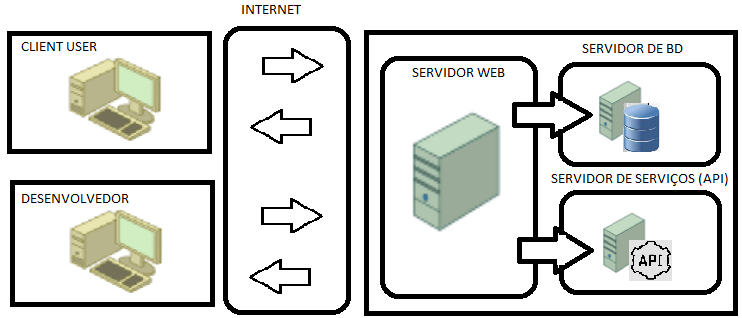
\includegraphics[scale=0.6]{08-arq_web.png}
	\caption{Esboço da arquitetura web}
\end{figure}

\subsubsection{Funções de um web service}

Um web server nada mais é que um software rodando em uma máquina. Ele desempenha várias funções que podemos elencar como:
\begin{itemize}
	\item Atender as requests http e responder a elas.
	\item Gerencias sites.
	\item Gerencias arquivos dos sites.
	\item Integrar mecanismos de scripts: php, perl, aspx, Ruby, Python e etc.
	\item Autenticar users (básica ou com servidores de autenticação).
	\item Implementar criptografia nas comunicações (https - tls/ssl).
	\item Cache de recursos.
	\item Auditoria das alterações e logs.
\end{itemize}

\subsubsection{Software e Provedores}

Basicamente, existem 3 formas de tornar uma aplicação web acessível aos clients: Rodar um web server na máquina local; instalar e configurar um wer server em uma máquina dedicada para esse trabalho e, por fim, contratar um provedor que ofereça esse serviço.
\\~\\
A lista de softwares que se propõe a fazer o trabalho de um web server é enorme. O material do curso elenca dois:
\begin{itemize}
	\item Apache HTTP Server | \href{https://httpd.apache.org/}{Apache Web Server} \\
			É um open source multi plataforma. Permite execução de multilinguagens como php, perl entre outras. Uma maneira simples de instalar é pelo \href{https://www.apachefriends.org/index.html}{XAMPP} (que já integra o apache web server, banco de dados MariaDB e um ambiente PHP e Perl).
	\item Microsoft Internet Information Server (IIS) \\
			É a solução proprietária da Microsoft. Baseado na plataforma .NET, permite hospedar sites estáticos. O IIS já vem disponível junto dos SO Windows.
\end{itemize}

A lista de provedores também é extensa  e possuem diferentes capacidades distintas mas podemos destacar algumas ferramentas úteis:
\begin{itemize}
	\item Servidores em Nuvem
	\begin{itemize}
		\item \href{https://azure.microsoft.com/pt-br/}{Azure}
		\item \href{https://www.heroku.com/}{Heroku}\footnote{Esse aqui eu to estudando e fazendo um manual de como usar. Você pode ler o manual nesse \href{https://github.com/brunoruas2/Analise_Des_Sistemas/tree/main/Manuals/heroku}{[LINK]}}
		\item \href{https://aws.amazon.com/pt/}{AWS}
	\end{itemize}

	\item Editores e IDEs online
	\begin{itemize}
		\item \href{https://replit.com/}{Replit}
		\item \href{https://codesandbox.io/}{CodeSandbox}
		\item \href{https://glitch.com/}{Glitch}
		\item \href{https://pages.github.com/}{GitHub Pages}
	\end{itemize}
\end{itemize}

\subsection{Dinâmica de Aplicações Web}

Quando você acessa um site, o arquivo que coordena o modo de exposição da informação e os conteúdos da mesma é um arquivo ``\verb|.html|''. Observe o exemplo abaixo de uma página simples.

\begin{Verbatim}[tabsize=4,frame=single]
<!DOCTYPE html>
<html lang="en">
	<head>
		<meta charset="UTF-8">
		<title>Document</title>
		<link rel="stylesheet" href="style.css">
		<script> src='app.js'</script>
	</head>
	<body>
		<img src='logo.jpg' alt="imagem_logo">
	</body>
</html>
\end{Verbatim}

As tags que contém as partes \verb|style.css|, \verb|app.js| e \verb|logo.jpg| fazem menção à outros arquivos que farão parte da composição da página. Alguns são referentes à funcionalidades ou layout da aplicação enquanto outros podem ser referentes à conteúdos mostrados na página.
\\~\\
Uma vez que o servidor compreende a request feita pelo client, ele envia uma série de arquivos que serão lidos pelo browser do usuário e serão interpretados por ele. O html é justamente o primeiro arquivo lido porque ele diz ao navegador quais conteúdos mostrar e, a partir das referências contidas no html, como mostrar e quais funcionalidades a página terá.

\subsubsection{O processamento de um site}

\begin{enumerate}
	\item O client envia uma requisição via http (com o método GET) para o web server
	\item O server envia o arquivo html da página requisitada para o browser
	\item Ao processar o html, o browser percebe que ele faz menção de outros arquivos (como css, js, mp3, etc)
	\item O browser faz novas requisições ao server até ter todos os arquivos necessários para o carregamento da página
\end{enumerate}

Como você pode ver, é muita coisa acontecendo. Só não nos damos conta disso porque o processo é muito rápido hoje em dia devida a velocidade das nossas conexões banda larga. Lembrando sempre que todas as requisições e respostas entre client e server são feitas usando-se o protocolo HTTP que a gente viu logo antes.

\section{Desenvolvimento de Interfaces Web}

\subsection{A Linguagem HTML}

A linguagem HTML foi criada por Tim Berners-Lee no ano de 1991 e foi baseada no padrão Standard Generalized Markup Language (SGML). Seu escopo original era para permitir a divulgação de pesquisas científicas.
\\~\\
Com o passar dos anos, novas tecnologias foram somadas ao ecossistema para facilitar o processo de construção das soluções web. O Cascading Style Sheet (CSS) foi criado para facilitar o desenvolvimento do conteúdo separando a parte de estilo e aparência do conteúdo em HTML. O JavaScript permitiu a manipulação de elementos além de dar mais dinâmica para as páginas web.
\\~\\
O W3C foi criado em 1993 e, a partir dessa data, o HTML foi mantido e padronizado por essa organização. Desde então a linguagem vem sendo alterada para permitir sua evolução.
\\~\\
Em 2004 foi criado o Web Hypertext Application Technology Working Group (WHATWG) por pessoas da Apple, Mozilla e Opera. Na época, o W3C estava trabalhando no padrão XHTML 2.0 (que iria substituir o HTML 4.01) mas o WHATWG conseguiu propor um monde que acabou sendo o HTML 5. O HTML 5 foi recebido e amplamente adotado no desenvolvimento de aplicações hoje em dia.
\\~\\
\textbf{Panorama de uma Aplicação}
\\~\\
Nós já sabemos que um client faz uma requisição ao web server por HTTP e esse, por sua vez, responde a requisição com, normalmente, um arquivo HTML. De posse de arquivo, o browser consegue saber se precisará solicitar mais arquivos ao web server até que todas as referências do HTML sejam satisfeitas e a página carregada.
\\~\\
A grosso modo, podemos dizer que o HTML pode fazer menções a arquivos dos seguintes tipos:
\begin{itemize}
	\item CSS
	\item Arquivos de Multimídia
	\item JavaScript
	\item RIA - Rich Internet Applications
		\begin{itemize}
			\item Applet Java
			\item Adobe Flash
			\item Adobe Air
			\item Adobe Flex
			\item SilverLight
		\end{itemize}
\end{itemize}

Se o site utiliza soluções dinâmicas como PHP, Java, Python, Ruby ou ASP.NET, quando a requisição é feita, o web server primeiro faz o processamento desses arquivos (normalmente por um outro servidor de APIs) e o resultado serão outros arquivos HTML, CSS, JS ou Multimídia. Após o processamento, o resultado é enviado para o client que será atualizado pelo browser.
\\~\\
Nas aplicações modernas, o seu browser está em processo praticamente contínuo de interação com o servidor e vice-versa.
\\~\\
\textbf{A Sintaxe da Linguagem HTML}
\\~\\
Uma página HTML é uma coleção de \textbf{elementos}. Você consegue identificá-los facilmente porque estão entre os pares de símbolos \verb|<>|. Cada elemento também tem uma tag de abertura e uma de fechamento. Por exemplo:

\begin{center}
	\verb|<body> Aqui vai o conteúdo do body </body>|
\end{center}

Também existem elementos que não precisam do par de tags de abertura e fechamento. Por exemplo:

\begin{center}
	\verb| <input disable name='Nome' value='rommelcarneiro'>|
\end{center}

Atente para o fato que alguns elementos aceitam outros elementos internamente. Por exemplo, dentro do elemento \verb|<body></body>| nós colocamos todos os outros elementos que comporão a nossa página web, como por exemplo, formulários, parágrafos, vídeos e etc. Então se acostume de termos elementos dentro de outros elementos.
\\~\\
Dentro de alguns elementos podem ser inseridas informações e configurações por meio de parâmetros que chamamos de \textbf{atributos} do elemento. Por exemplo, no elemento logo acima, temos os atributos \verb|name| e \verb|value|.
\\~\\
Agora que sabemos o que são elementos e como eles são construídos, podemos seguir para a \textbf{organização de um documento HTML}. Existe um padrão em todo arquivo HTML onde existem alguns elementos obrigatórios para o processamento da página pelo browser do client.

\begin{Verbatim}[tabsize=4,frame=single]
<!DOCTYPE html> -----------------> Elemento da versão do HTML
<html lang="en"> ----------------> Abertura do documento HTML 
	<head> ----------------------> Abertura do cabeçalho      
		<meta charset="UTF-8"> --> Atributo nome = "valor"    
		<title>Document</title> -> Elemento de Título         
	</head> ---------------------> Fechamento do cabeçalho
	<body> ----------------------> Abertura do corpo
		<img src="logo.jpg"> ----> Elemento de imagem         
	</body> ---------------------> Abertura do corpo
</html> -------------------------> Fechamento do HTML
\end{Verbatim}

\textbf{Preâmbulo}
\\~\\
Como podemos ver, primeiro temos o preâmbulo \verb|DOCTYPE|, seguido do \verb|<html> </html>| onde temos outros dois elementos maiores, o cabeçalho (\verb|<head> </head>|) e o corpo (\verb|<body> </body>|).
\\~\\
O preâmbulo diz ao navegador qual versão da HTML será usada. Se ele não for indicado, o navegador vai tentar ``adivinhar'' qual a melhor maneira de interpretar a sua página (chamamos isso de \textbf{quirks mode}). Caso você informe qual a versão, o browser usará o processamento adequado (chamamos de \textbf{strict mode}). Os formatos do preâmbulo mudam de acordo com a versão do HTML:

\footnotesize
\begin{itemize}
	\item HTML 5 \\
	\verb|<!DOCTYPE html>|
	\item HTML 4.01 \\
	\verb|<!DOCTYPE HTML PUBLIC "-//W3C//DTD HTML 4.01 Transitional//EN"| \\
	\verb|"http://www.w3.org/TR/html4/loose.dtd">|
	\item HTML 1.0 \\
	\verb|<!DOCTYPE html PUBLIC "-//W3C//DTD XHTML 1.0 Transitional//EN"| \\
	\verb|"http://www.w3.org/TR/xhtml1/DTD/xhtml1-transitional.dtd">|
\end{itemize}
\normalsize

\textbf{Cabeçalho}
\\~\\
É a primeira parte dentro da tag de html. Nele estão as informações sobre o documento de modo a organizar as referências de funcionalidade que serão usadas para o processamento da página web. Podemos resumir os elementos no cabeçalho como:
\begin{itemize}
	\item title - \verb|<title> </title>| \\
		Define o título do documento. Que também afeta a aba do navegador.
	\item link - \verb|<link rel="relacao" href="link_do_arquivo.extensao">| \\
		Define as ligações externas como arquivos, scripts, CSS e etc. 
	\item style - \verb|<link rel="stylesheet" href="style.css">| \\
		É um tipo de link. Nele é que vamos indicar qual o arquivo que regerá o layout da nossa aplicação.
	\item meta - \verb|meta name="nome" content="conteudo">| \\
		Aqui teremos as informações adicionais sobre a página: codificação de caracteres, descrição, palavras-chaves, autor e etc.
\end{itemize}

\textbf{Corpo}
\\~\\
A segunda parte do html é o corpo. Nele é onde colocamos o conteúdo que fará parte da página. Como é muito comum de se encontrar nos sites, esse conteúdo pode vir mesclado em várias mídias como texto, imagens, vídeos, mapas e etc. Veremos com calma um pouco mais a frente.

\subsubsection{Elementos de Texto e Multimídia}

Como esse material tem o objetivo de ser para futuras consultas. Eu vou colocar as tags com um pequeno resumo mas não vou comentar muito sobre elas.
\\~\\
\textbf{Parágrafos e Títulos}

\begin{center}
	\begin{tabular}{|c|c|}
		\hline
		\textbf{Elemento} & \textbf{Tags} \\
		\hline
		\hline
		Títulos & \verb|<h1></h1>,...,<h6></h6>| \\
		\hline
		Parágrafo & \verb|<p></p>| \\
		\hline
		Quebra de Linha & \verb|<br>| \\
		\hline
		Itálico & \verb|<i></i>| \\
		\hline
		Negrito & \verb|<b></b>| \\
		\hline
		Importância & \verb|<strong></strong>| \\
		\hline
		Código-fonte & \verb|<code></code>| \\
		\hline
		Texto pre-formatado & \verb|<pre></pre>| \\
		\hline
		Citações & \verb|<blockquote></blockquote>| \\
		\hline
	\end{tabular}
\end{center}

Enquanto estamos montando a nossa página html, devemos evitar usar os elementos dela para a formatação de layout da nossa solução. É altamente recomendado deixar toda essa responsabilidade para a nossa Cascading Style Sheets (CSS) e focar apenas no conteúdo textual da página web.
\\~\\
\textbf{Listas}
\\~\\
Existem 3 tipos de listas em HTML.
\\~\\
Listas ordenadas:
\begin{Verbatim}[tabsize=4,frame=single]
<ol>
	<li> Primeiro item </li> --------> 1. Primeiro item
	<li> Segundo item </li> ---------> 2. Segundo item
	<li> Terceiro item </li> --------> 3. Terceiro item
</ol>
\end{Verbatim}

Lista não ordenada:
\begin{Verbatim}[tabsize=4,frame=single]
<ul>
	<li> Primeiro item </li> --------> o Primeiro item
	<li> Segundo item </li> ---------> o Segundo item
	<li> Terceiro item </li> --------> o Terceiro item
</ul>
\end{Verbatim}

Lista de definições:
\begin{Verbatim}[tabsize=4,frame=single]
<dl>
	<dt> Termo 01 </li> -------------> Termo 01
	<dd> Definição 01 </li> ---------> 		Definição 01
	<dt> Termo 02 </li> -------------> Termo 02
	<dd> Definição 02 </li> ---------> 		Definição 02
</dl>
\end{Verbatim}

\textbf{Imagens}
\begin{Verbatim}[tabsize=4,frame=single]
	<img width="200" height="180" src="img.png" alt="Peixe">
\end{Verbatim}

\textbf{Links}
\footnotesize
\begin{Verbatim}[tabsize=4,frame=single]
<a href="link.com" target="_blank"> Texto </a> ------> Nova tab
<a href="link.com" target="_self"> Texto </a> -------> Mesma tab
<a href="link.com" target="_parent"> Texto </a> -----> Frame pai
<a href="link.com" target="_top"> Texto </a> --------> Janela atual
<a href="link.com" target="nome_frame"> Texto </a> --> Frame nominado
\end{Verbatim}
\normalsize

\subsubsection{Elementos Estruturais}

A partir da versão 4.0 o principal elemento usado para segmentar as partes de uma página html passou a ser o \verb|<div>| que é um um elemento de divisão genérico para agrupar qualquer conjunto de elementos necessários. Por exemplo:

\begin{Verbatim}[tabsize=4,frame=single]
<div>
    <h1> Titulo </h1>
    <p> Parágrafo pequeno </p>
    <ol>
        <li>Item</li>
        <li>Item</li>
    </ol>
</div>
\end{Verbatim}

Na versão 5 do HTML passamos a ter vários tipos de elementos com a mesma função dos \verb|<div>| mas agora com nomes mais fáceis de usar. As vezes nos referimos a eles como \textbf{elementos semânticos}. O novos elementos semânticos apresentados na versão 5 do html são:

\begin{center}
	\begin{tabular}{|c|c|}
		\hline
		\textbf{Elementos} & \textbf{Descrição} \\
		\hline
		\hline
		\verb|<article>| & Define um artigo \\
		\hline
		\verb|<aside>| & Conteúdo ao lado da página \\
		\hline
		\verb|<details>| & Detalhes adicionais \\
		\hline
		\verb|<figcaption>| & Título para \verb|<figure>| \\
		\hline
		\verb|<figure>| & Elemento autocontido \\
		\hline
		\verb|<footer>| & Rodapé para seção \\
		\hline
		\verb|<header>| & Cabeçalho para seção \\
		\hline
		\verb|<main>| & Conteúdo principal \\
		\hline
		\verb|<mark>| & Texto destacado \\
		\hline
		\verb|<nav>| & Conteúdo de navegação \\
		\hline
		\verb|<section>| & Seção do documento \\
		\hline
		\verb|<summary>| & Resumo \\
		\hline
		\verb|<time>| & Define data/hora \\
		\hline	
	\end{tabular}	
\end{center}

Quando construímos a estrutura do nosso site apenas com elementos \verb|<div>| genéricos, nós não estamos indicando nenhuma relação entre essas seções. Quando usamos a divisão via elementos semânticos, permitimos um processamento por algoritmos de modo a abrir todo um leque de possibilidades de interações a partir disso. Esse é um dos motivos que justificam o nome da web 3.0 como sendo \textbf{web semântica}. 
\\~\\
Abaixo temos duas maneiras de representar uma estrutura de um site. A primeira em estrutura genérica de \verb|div| e a outra em elementos semânticos. Veja como a segunda abordagem é mais simples de ler.

\begin{figure}[H]
	\centering
	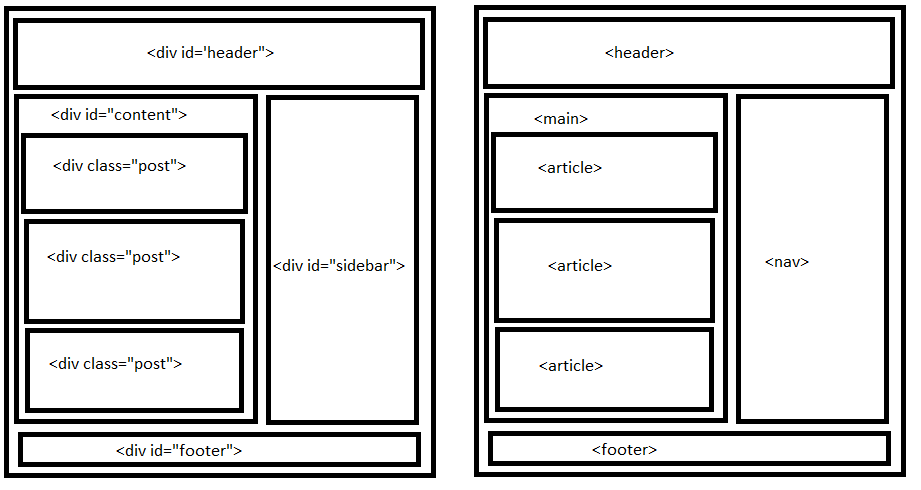
\includegraphics[scale=0.5]{09-divs_semantic.png}
	\caption{Estrutura em <div> versus Estrutura em elementos semânticos}
\end{figure}

Não é difícil perceber que o uso de elementos semânticos é fortemente indicado para o desenvolvimento de aplicações web modernas.

\subsubsection{Elementos de Tabelas}

Não é nada incomum ter que demonstrar dados usando uma tabela. Pensando nisso, a linguagem HTML também possui um elemento especificamente criado para criação de tabelas. Uma tabela pode ser criada com o uso das seguintes tags:

\begin{Verbatim}[tabsize=4,frame=single]
<table border="1"> --------------> Cria a Tabela
	<caption> Título </caption> -> Coloca um Título
	<tr> ------------------------> Table Row (tr)
		<td>L1C1</td> -----------> Table Data Column 1
		<td>L1C2</td> -----------> Table Data Column 2
	</tr>
	<tr>
		<td>L2C1</td> -----------> Table Data Column 1
		<td>L2C2</td> -----------> Table Data Column 2
	</tr>
</table>
\end{Verbatim}

Existem vários elementos que podem ser usados dentro de uma tabela. São os principais:

\begin{center}
	\begin{tabular}{|c|c|}
		\hline
		\textbf{Elementos} & \textbf{Descrição} \\
		\hline
		\hline
		\verb|<table>| & Elemento que cria a tabela \\
		\hline
		\verb|<caption>| & Título da tabela \\
		\hline
		\verb|<thead>| & Linhas do cabeçalho \\
		\hline
		\verb|<tbody>| & Linhas do body \\
		\hline
		\verb|<tfoot>| & Linhas do rodapé \\
		\hline
		\verb|<tr>| & Linha da tabela \\
		\hline
		\verb|<th>| & Cabeçalho dentro de uma linha \\
		\hline
		\verb|<td>| & Table data \\
		\hline
	\end{tabular}
\end{center}

\textbf{Comentário:} Não podemos cair na tentação de usar tabelas como ferramenta de layout da página. Pode até parecer mais simples no começo mas tabelas não são boas para criação de aplicações fluidas e dinâmicas.

\subsubsection{Elementos de Formulários}

Uma das interações mais básicas que precisamos de um usuário é a inserção de dados na aplicação. Dentre as várias maneiras de conseguirmos um dado inserido pelo usuário, o formulário é a mais simples.
\\~\\
O HTML fornece vários atributos dentro do elemento \verb|<form></form>| que nos permite a criar campos de texto, botões clicáveis, campos de senha e etc. A sintaxe mais básica de um formulário é dada por:

\begin{Verbatim}[tabsize=4,frame=single]
<form name="form_name" action="login.html" method="POST">
	Usuário: <br>
	<input type="text" name="user" value=""> <br>
	Senha: <br>
	<input type="password" name="psw" value=""> <br> <br>
	<input type="submit" value="OK">
</form>
\end{Verbatim}

Podemos usar o atributo \textbf{name} ou \textbf{id} para identificar o nosso formulário\footnote{Isso é muito importante porque vamos usar essa informação para fazer alguma coisa.}. O atributo \textbf{action} indica qual URL vai ser disparada uma vez processado o form (no nosso exemplo seria algo como \verb|http://server.com/login.html|). O atributo \textbf{method} indica o método HTTP de submissão dos dados do formulário no nosso bando de dados (pode ser \verb|POST| ou \verb|GET|).
\\~\\
Quando o método usado for o \verb|GET|, o browser faz uma requisição da \verb|URL| indicada para o servidor passando os parâmetros de input como \textbf{querystring} na URL. No nosso exemplo, ficaria como \verb|http://server.com/login.html/| \verb|login.html?user=texto&psw=123|.
\\~\\
Quando o método escolhido é o \verb|POST|, os dados são enviados ao servidor no corpo da requisição HTTP e não aparecem na URL. A essa altura você já deve ser capaz de entender as diferenças entre esses dois métodos.
\\~\\
\textbf{Elemento} \verb|<input>|
\\~\\
Esse elemento é bastante utilizado na composição dos formulários (na verdade, eu nem consigo pensar em um formulário sem pelo menos um input). Ele define os campos ou entradas de informação e possui os seguintes atributos:
\begin{itemize}
	\item \verb|type| - Cada tipo de input possui uma visualização diferente quando a página é carregada. Isso é feito para permitir uma melhor interação do usuário de acordo com a natureza da informação requerida. As opções são:
		\begin{itemize}
			\item text - Campo de texto aberto. A quantidade de caracteres pode ser controlada pelo atributo \verb|maxlength|.
			\item number - Só aceita número como input e permite a seleção por umas setinhas que aparecem ao lado do campo.
			\item password - Igual ao campo texto mas com os caracteres anonimizados.
			\item email - Confere se o texto inserido possui um @ antes de salvar o formulário.
			\item date - Coloca uma máscara no formato de data e cria uma opção de input por calendário.
			\item radio button - Uma opção clicável com um valor associado e um nome. O navegador só permite que um único radio button esteja selecionado se existir mais de uma opção com o mesmo nome no atributo \verb|name|.
			\item checkbox - Mesma lógica do radio button mas com permissão de vários selecionados simultaneamente.
			\item submit - É um botão clicável que normalmente dispara a informação do formulário ao servidor web ou a um script JS local.
			\item reset - É igual um submit mas a única função dele é apagar tudo que foi preenchido no formulário.
		\end{itemize}
	\item \verb|name| - Nome de identificação do campo.
	\item \verb|value| - Valor contudo no campo.
	\item \verb|placeholder| - Valor que aparece quando o campo estiver vazio.
	\item \verb|required| - Validação automática para evitar o não preenchimento do campo antes da submissão do form.
	\item \verb|disabled| - Inativa o campo e não permite interação mas o user ainda poderá ver.
\end{itemize}

Na imagem abaixo podemos ver como cada tipo do elemento \verb|<input>| aparece para um usuário:

\begin{figure}[H]
	\centering
	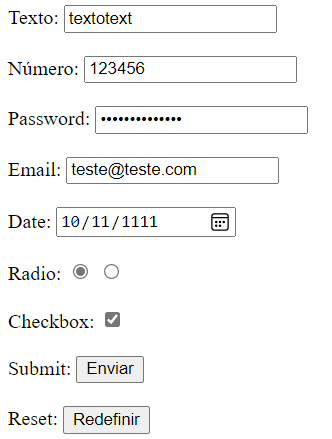
\includegraphics[scale=0.4]{10-forms.png}
	\caption{Tipos de elementos <input> dentro de um formulário html.}
\end{figure}

\textbf{Elemento} \verb|<textarea>|
\\~\\
Esse é tranquilo de entender. Sempre que precisarmos de um input de texto maior do que uma linha, podemos usar o elemento \verb|<textarea name="" rows="10"| \verb|cols="50"></textarea>| para isso. É possível alterar a quantidade de linhas e a número de colunas para apresentação da nossa caixa de texto apenas mudando os parâmetros dos atributos.
\\~\\
\textbf{Elemento} \verb|<select>|
\\~\\
Podemos permitir que o usuário selecione uma lista pré-selecionada de opções através de uma \textbf{lista em caixa} (também chamada de \textbf{dropdown menu}). Um exemplo de código contendo esse elemento por ser visto abaixo.

\begin{Verbatim}[tabsize=4,frame=single]
<label for="lista"> Dropdown Menu </label>
<select name="lista">
	<option value="">Selecione uma opção</option>
	<option value="01">Opção 01</option>
	<option value="02">Opção 02</option>
	<option value="03">Opção 03</option>
	<option value="04">Opção 04</option>
	<option value="05">Opção 05</option>
</select>	
\end{Verbatim}

É possível transformar a lista suspensa em uma lista fixa que permite mais de uma seleção. Para fazer isso é só adicionar o atributo \verb|multiple| e também o atributo \verb|size=| no elemento \verb|select|.
\\~\\
Perceba que além do elemento de lista nós trouxemos um novo elemento chamado \verb|label| que adiciona um texto associado a algum elemento. No nosso exemplo, veja como foi indicado no atributo \verb|for| o mesmo nome que o atributo \verb|name| recebe dentro do elemento \verb|select|.
\\~\\
O resultado pode ser visto abaixo:

\begin{figure}[H]
	\centering
	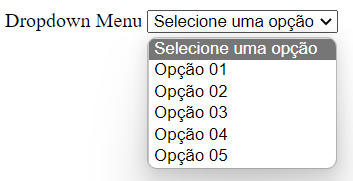
\includegraphics[scale=0.6]{11-dropdown.png}
	\caption{Tipos de elementos <input> dentro de um formulário html.}
\end{figure}

\subsection{A Linguagem CSS}

Nós falamos na parte inicial do nosso estudo sobre HTML, mas especificamente na parte do cabeçalho, que uma das referências que normalmente fazemos é a de uma \textbf{Cascading Style Sheet (CSS)}. A ideia por trás disso é que a manutenção e o desenvolvimento da aplicação web fica mais simples quando trabalhamos todo o aspecto de estilo visual em um arquivo separado (.css) do arquivo que trata da estrutura da aplicação (.html).
\\~\\
Contudo, na realidade, existem outras formas de trabalhar o visual da aplicação além do arquivo .css em separado. No geral, podemos dizer que existem 3 formas de gerenciamento de estilo de um aplicação web:
\begin{itemize}
	\item CSS externo - Melhor forma. Nosso material estará focado nesse tipo de arquitetura.
	\item Bloco interno - As regras ficam no próprio arquivo html. Pode ter aplicações para questões muito específicas. Mas as atualizações vão precisar ser feitas em cada página, sempre que necessário.
	\item Atributo inline - Pior forma. Aqui, as regras de estilo são definidas diretamente no elemento html. Qualquer mínima alteração terá de ser feita diretamente no elemento e em todas as páginas.
\end{itemize}

Aqui podemos ver um exemplo de cada aplicação do estilo visual que elencamos acima:
\scriptsize
\begin{Verbatim}[tabsize=4,frame=single]
<!DOCTYPE html>
<html lang="en">
<head>
	<title>Exemplo CSS</title>

	###Esse é um exemplo de arquivo externo###
	<link rel="stylesheet" href="style.css" type="text/css">

	###Exemplo de bloco interno####
	<style type="text/css">
		p {
			font-size: 10pt;
			font-family: "Verdana";
			color: blue;
		  }
		
		h1 { font-size: 16pt; 
			 font-family: "Impact"; 
			 color: red;
			}
	</style>

</head>
<body>
	####Exemplo de inline#####
	<p style="margin-left: 0.5in; font-size: 8pt;">
		Texto do parágrafo
	</p>
</body>
</html>
\end{Verbatim}
\normalsize

A prioridade de leitura das regras de estilo que o browser vai usar é 1) inline, 2) Bloco interno, 3) CSS externo e 4) Default do navegador.
\\~\\
\textbf{Sintaxe da linguagem CSS}
\\~\\
A leitura de um arquivo CSS é bem simples. A primeira coisa que precisamos saber é quais elementos estão presentes no html que será trabalhado e quais desses elementos possuem atribuição de id específico. 
\\~\\
Por exemplo, se tivermos no nosso html dois elementos \verb|<p>|, só que um deles possui o atributo id \verb|<p id="teste">|. Para criarmos uma regra de estilo no nosso CSS basta escrevermos a tag do elemento (sem os símbolos \verb|<>|) do seguinte modo.

\begin{Verbatim}[tabsize=4,frame=single]
p {
	color: red;
}
\end{Verbatim}

Essa regra diz que todos os textos contidos nos elementos \verb|<p>| terão a cor vermelha. Contudo, se quisermos adotar uma regra específica para apenas um elemento em questão, podemos definir a regra no css diretamente para o elemento com o seu id.

\begin{Verbatim}[tabsize=4,frame=single]
#teste {
	color: black;
}
\end{Verbatim}

Isso nos dará uma página onde todos os textos dos parágrafos serão vermelhos à exceção do parágrafo identificado pelo \verb|id="teste"|.
\\~\\
Podemos resumir a sintaxe do CSS como sendo:

\begin{Verbatim}[tabsize=4,frame=single]
seletor { 
	propriedade_1 : valor_da_propriedade_1; 
	propriedade_2 : valor_da_propriedade_2;
	...
	propriedade_n : valor_da_propriedade_n;
}
\end{Verbatim}

Ou seja, para aprender bem CSS, vamos precisar aprender as várias maneiras de selecionar os elementos da página html e as propriedades de estilo que o CSS nos permite manipular na construção das nossas aplicações web.

\subsubsection{Seletores de Elementos}

Eu já adianto, existem muitos tipos de seletores. Nós precisamos decorar todos os tipos? Evidente que não. O importante é saber que o estilo de uma aplicação pode ser desenvolvido de várias maneiras e que, quanto melhor for o método de organização do CSS, mais fácil será o desenvolvimento e a manutenção da aplicação no futuro. A tabela a seguir é uma referência para os vários tipos de seletores em CSS.

\footnotesize
\begin{center}
\begin{tabular}{|c|c|c|}
	\hline
	\textbf{Tipo} & \textbf{Link com HTML} & \textbf{Exemplo de Sintaxe} \\
	\hline
	\hline
	Elemento & Nome da tag html & \verb|p {color:blue;}| \\
	\hline
	Identificador & id dos elementos & \verb|#ident {color:blue;}| \\
	\hline
	Classe & Classe dos elementos & \verb|.classe {color:blue;}| \\
	\hline
	Atributo & Atributos dos elementos  & \begin{tabular}{lll}
		\verb|[atrib] {color:blue;}| \\
		\verb|[id="p01"] {color:blue;}| \\
		\verb|[class~="marked" {color:blue;}| \\
	\end{tabular} \\
	\hline
	Pseudo-Classe & Situações dos elementos  & \begin{tabular}{lll} 
		\verb|p:first-of-type {color:blue;}| \\ 
		\verb|p:nth-child(3) {color:blue;}| \\ 
		\verb|:hover {color:blue;}| \\
	\end{tabular} \\
	\hline
	Pseudo-Elemento & Partes de elementos & \begin{tabular}{lll}
		\verb|p::first-letter {color:blue;}| \\
		\verb|p::first-time {color:blue;}| \\
		\verb|p::after {color:blue;}| \\
	\end{tabular} \\
	\hline
	Universal & Todos os elementos & \verb|* {color:blue;}| \\
	\hline
\end{tabular}
\end{center}
\normalsize

Podemos ver que existem vários modelos de seletores para os elementos html de um página. Alguns deles são dependente de contexto de interação do elemento. Especialmente, as situações de pseudo-classe são muito úteis para criação de aplicações fluidas e avançadas.
\\~\\
Link para lista de todos os pseudo-elementos e pseudo-classes suportados pelo CSS atualmente: \href{https://developer.mozilla.org/en-US/docs/Learn/CSS/Building_blocks/Selectors/Pseudo-classes_and_pseudo-elements}{[LINK]}.
\\~\\
\textbf{Combinação de Seletores}
\\~\\
Podemos usar combinações de seletores para definir as regras de estilo das nossas aplicações web. Essas combinações obedecem a determinadas regras que devem ser seguidas para se obter o resultado esperado. Abaixo segue uma tabela de referência.

\begin{center}
\begin{tabular}{|c|c|}
	\hline
	\textbf{Regra} & \textbf{Interpretação} \\
	\hline
	\hline
	\verb|A,B {...}| & Aplica a mesma regra em A e B \\	
	\hline
	\verb|A.B {...}| & classes e ids associados à A e B ao mesmo tempo \\	
	\hline
	\verb|A B {...}| & Elementos em B que também pertençam a A \\	
	\hline
	\verb|A > B {...}| & Elementos em B filhos de elementos de A \\	
	\hline
	\verb|A + B {...}| & Elemento em B próximo irmão de elementos de A \\	
	\hline
	\verb|A ~ B {...}| & Elementos em B próximos irmãos de elementos de A \\
	\hline
\end{tabular}
\end{center}
\ 
\\~\\
\textbf{Prioridade de Seletores}
\\~\\
O processamento das declarações CSS obedecem a ordem em 3 regras:
\begin{itemize}
	\item O processamento é de cima para baixo. A última declaração é a que prevalecerá.
	\item Regras específicas são prioridade em relação à regras gerais.
	\item As declarações marcadas como importantes \verb|p {color: red !important;}| são prioritárias.
\end{itemize}

\subsubsection{Valores e Unidades}

Atenção aqui. Entender bem quais unidades podem ser usadas e os tipos de unidades ajuda muito o desenvolvimento de interfaces bem planejadas e responsivas.
\\~\\
\footnotesize
\begin{center}
\begin{tabular}{|c|c|c|c|}
	\hline
	\textbf{Tipo} & \textbf{Medida} & \textbf{Significado} & \textbf{Observação} \\
	\hline
	\hline
	Absoluto & \begin{tabular}{lllll}
		in \\
		\hline
		cm \\
		\hline
		mm \\
		\hline
		pt \\
		\hline
		pc \\
	\end{tabular} & \begin{tabular}{lllll}
		Polegadas \\
		\hline
		Centímetros \\
		\hline
		Milímetros \\
		\hline
		Pontos \\
		\hline
		Paicas \\
	\end{tabular} & \\
	\hline
	Relativo & \begin{tabular}{lll}
		em \\ \ \\
		\hline
		px \\ \ \\
		\hline
		\% \\
	\end{tabular} & \begin{tabular}{lll}
		Tamanho da fonte \\ \ \\
		\hline
		Pixels \\ \ \\
		\hline
		Percentual \\
	\end{tabular} & \begin{tabular}{lll}
		1.2em é equivalente a \\ 
		120\% do tamanho original. \\
		\hline
		Um ponto no display onde \\
		a página é exibida. \\
		\hline
		120\% é a mesma coisa que 1.2 em. \\
	\end{tabular} \\
	\hline
\end{tabular}
\end{center}
\normalsize
\ 
\\~\\
\textbf{Cores em CSS}
\\~\\
Existem infinitas combinações de cores para a paleta que será usada em qualquer aplicação web. Existem diferentes maneiras de definir quais cores serão usadas em CSS:
\begin{itemize}
	\item RGB hexadecimal - \#RRGGBB
	\item RGB abreviado - \#RGB
	\item RGB decimal - rgb(rrr,ggg,bbb)
	\item Palavras-Chaves
\end{itemize}

Podemos usar qualquer uma dessas codificações para definir as cores que vamos usar no estilo das nossas aplicações web.

\subsubsection{Display e Box Model}

Um dos aspectos mais importantes na construção de uma aplicação web é a disposição dos elementos. Agora que aprendemos como a linguagem CSS nos fornece uma maneira mais simples de controlar as informações de estilo da nossa página HTML, vamos aprender como controlamos os locais onde os elementos são dispostos.
\\~\\
A propriedade display é que determina como um elemento e seus filhos são dispostos na página. Alguns valores dessa propriedade se referem a maneira como o elemento é organizado em relação aos elementos irmãos e alguns valores se referem a maneira como seus elementos filhos são dispostos dentro do elemento pai.
\\~\\
Caso não coloquemos nenhuma informação de display nos elementos, eles possuem uma categoria default própria que pode ser do tipo \verb|inline| ou \verb|block|.
\\~\\
Os elementos \verb|inline| são colocados automaticamente um ao lado do outro na mesma linha enquanto existir espaço na tela.

\begin{itemize}
	\item \verb|<a>|
	\item \verb|<span>|
	\item \verb|<img>|
	\item \verb|<button>|
	\item \verb|<input>| 
	\item etc
\end{itemize}

Os elementos \verb|block| sempre ocupam uma linha inteira da página. 
\begin{itemize}
	\item \verb|<div>|
	\item \verb|<h1>| \dots \verb|<h6>|
	\item \verb|<p>|
	\item \verb|<form>|
	\item \verb|<canvas>|
	\item \verb|<table>|
	\item etc
\end{itemize}

Mais ou menos como nessa imagem abaixo

\begin{figure}[H]
	\centering
	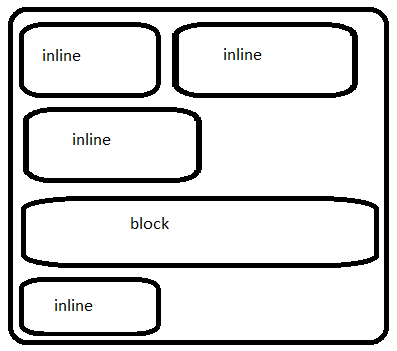
\includegraphics[scale=0.6]{12-display.png}
	\caption{Exemplo de elementos inline e block.}
\end{figure}

Podemos modificar o comportamento padrão de um elemento através do parâmetro \verb|display:| no CSS. Por exemplo, para transformar os \verb|<input>| em um elemento sozinho na página, podemos colocar no CSS a seguinte linha

\begin{Verbatim}[tabsize=4,frame=single]
input { 
	display: block; 
	margin: 0 auto; 
}
\end{Verbatim}

No caso de elementos inside\footnote{também chamados de elementos filhos.}, o atributo display pode receber os valores \verb|display="table"|,\verb|display="grid"| e \verb|display="flex"|. Quando colocamos esses atributos nos elementos inside, o elemento que o contém, que chamamos de elemento pai (outside), automaticamente vira um elemento do tipo \verb|display="block"|.
\\~\\
A propriedade \verb|display="table"| em um elemento outside permite que os elementos inside recebam variações desse atributo para a construção de layout em formato de tabela. Desse modo, se nosso elemento outside é do tipo \verb|display="table"|, então, os elementos inside podem ser \verb|"table-row"|, \verb|"table-cell"|, \verb|"table-column"|, \verb|"table-caption"|, \verb|"table-row-group"|, \verb|"table-header-group"| e \verb|"table-footer-group"|.
\\~\\
A propriedade \verb|display="flex"| permite que os elementos inside sejam controlados de maneira fluida para se ajustar à largura da janela do navegador.
\\~\\
A propriedade \verb|display="grid"| permite um controle das regiões onde os elementos inside serão dispostos. Isso dá mais controle ao desenvolver.
\\~\\
Veremos com mais calma os atributos \verb|display:flex| e \verb|display:grid| porque eles são usados na construção de aplicações mais fluidas e dinâmicas.
\\~\\
\textbf{Box Model}
\\~\\
Existe um conjunto de atributos CSS que compõe o que podemos chamar de \textbf{box model}. A ideia aqui é que podemos trabalhar os elementos como pertencentes a uma ``caixa'' imaginária. Isso torna o design da aplicação mais simples de compreender e também facilita o posicionamento dos elementos ao longo da nossa página.
\\~\\
Os atributos CSS que compõe o modelo de caixa são:
\begin{itemize}
	\item \verb|margin| 
	\item \verb|border|
	\item \verb|padding|
	\item \verb|width|
	\item \verb|height|
	\item \verb|background-color|
\end{itemize}

As propriedades de \verb|margin|, \verb|border| e \verb|padding| aceitam atributos de orientação como \verb|top-right-bottom-left|. Caso queira aplicar o mesmo valor para todos é só informar um único valor no atributo. Se quiser discriminar, é só apontar os valores na ordem descrita no sentido horário ou usar a propriedade inteira para cada lado. A imagem abaixo deixa mais fácil a compreensão do atributos do modelo de caixa.

\begin{figure}[H]
	\centering
	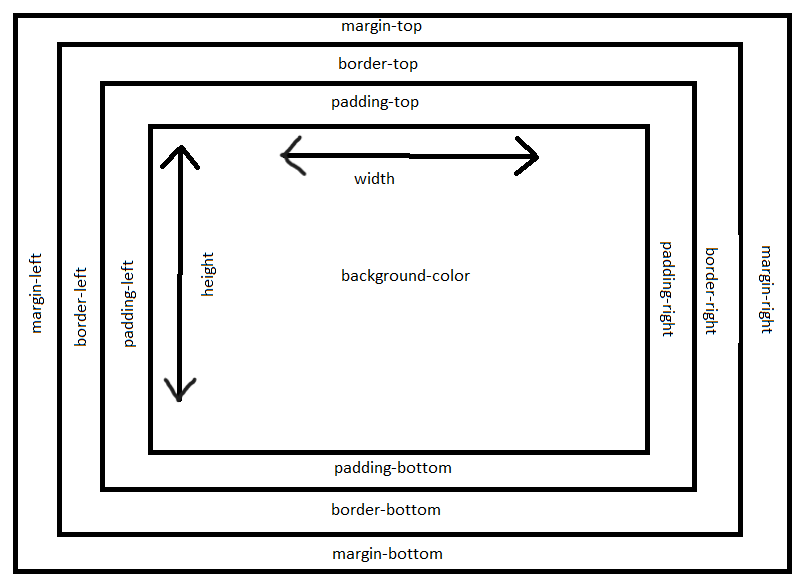
\includegraphics[scale=0.6]{13-box-model.png}
	\caption{O Box Model do CSS.}
\end{figure}

Durante a elaboração da interface não é nada incomum usar as bordas como método de visualização. O comando que cria a borda é
\begin{center}
	\verb|border: solid 20px black|.
\end{center}
\ 
\\~\\
\textbf{Fundo de Elementos (Background)}
\\~\\
Todo elementos html possui um atributo de background que pode ser acessado pelos seguintes comandos:
\begin{itemize}
	\item \verb|background-color| - Cor de fundo
	\item \verb|background-image| - Imagem ou gradiente\footnote{Você pode pesquisar para saber a lista dos gradientes disponíveis.}
	\item \verb|background-repeat| - Comando caso a img não seja do tamanho do elemento. Pode ser do tipo \verb|repeat|, \verb|repeat-x|, \verb|repeat-y|, \verb|space|, \verb|round|
	\item \verb|background-position| - Define a posição inicial da imagem. Pode ser do tipo \verb|top|, \verb|left|, \verb|right|, \verb|center|, \verb|bottom|
\end{itemize}

\subsubsection{Propriedades de Texto}

Existem várias propriedades quando o assunto é texto em CSS. Abaixo podemos ver uma tabela para referência.

\scriptsize
\begin{center}	
\begin{tabular}{|c|c|c|}
	\hline
	\textbf{Propriedade} & \textbf{Descrição} & \textbf{Valores} \\
	\hline
	\hline
	\verb|font-family| & Tipo de fonte &  aria | helvetica | sans-serif \\
	\hline
	\verb|font-size| & Tamanho da Letra & \begin{tabular}{llll}
		 xx-small | x-small | small  \\ 
		 medium | large | x-large   \\ 
		 xx-large | smaller | larger  \\
		 10px | 80\%
	\end{tabular} \\
	\hline
	\verb|font-style| & Estilo da fonte & normal | italic | oblique \\
	\hline
	\verb|font-weight| & Largura & normal | bold | bolder | 100 \\
	\hline
	\verb|font-variant| & \begin{tabular}{ll}
		Minúsculas como \\ maiúsculas menores
	\end{tabular} & normal | small-caps \\
	\hline
	\verb|line-height| & Altura & normal | 1.6 | 80\% \\
	\hline
	\verb|color| & Cor do texto &  [cor] \\
	\hline
	\verb|text-align| & Alinhamento & left | right | center | justify \\
	\hline
	\verb|text-shadow| & Sombra & \begin{tabular}{llll}
		x y z [cor] \\
		x - horizontal \\
		y - vertical \\
		z - difusão da sombra
	\end{tabular}\\
	\hline
	\verb|text-decoration-line| & Tipo de decoração & underline | overline |line-through \\
	\hline
	\verb|text-decoration-style| & \begin{tabular}{ll}
		Tipo de linha \\ de decoração
	\end{tabular} & solid | wavy | dashed | dotted | double \\
	\hline
	\verb|text-decoration-color| & \begin{tabular}{ll}
		Cor da linha \\ de decoração
	\end{tabular} & [cor] \\
	\hline
	\verb|letter-spacing| & \begin{tabular}{ll}
		Espaçamento das \\ letras
	\end{tabular} & normal  | 2px | 0.1em \\
	\hline
	\verb|word-spacing| & \begin{tabular}{ll}
		Espaçamento das \\ palavras
	\end{tabular} & normal  | 2px | 0.1em \\
	\hline
	\verb|text-transform| & \begin{tabular}{ll}
		Tipo de escrita \\ do texto
	\end{tabular} & capitalize | uppercase | lowercase \\
	\hline		
\end{tabular}
\end{center}
\normalsize
\ 
\\~\\
\textbf{Fontes de Texto na Web}
\\~\\
O CSS nos dá as seguintes opções de letras: serif, sans-serif,monospace, cursive e fantasy. Contudo, nós nunca teremos certeza se o navegados do user terá a capacidade de carregar a fonte que desejamos. Para evitar esse problema, podemos definir opções de fontes do seguinte modo:

\begin{center}
\begin{Verbatim}[tabsize=4,frame=single]
p {
	font-family: "Trebuchet MS", Verdana, sans-serif;
}		
\end{Verbatim}
\end{center}

O navegador do user vai tenter renderizar a página usando a primeira opção, caso ele não consiga, ele vai para as outras opções.
\\~\\
Além das opções padrão CSS, podemos usar fontes proprietárias de outras fontes (Google Fonts, DaFont, Adobe e etc). A maneira de fazer isso é definir uma propriedade de importação como no exemplo abaixo

\begin{Verbatim}[tabsize=4,frame=single]
@import url('https://fonts.googleapis.com/css?family=Baloo');

div {
	font-family: 'Baloo', cursive;
}
\end{Verbatim}

\subsubsection{Layouts Responsivos}

Não é nada incomum acharmos sites que respondem dinamicamente ao tamanho da tela. Agora vamos aprender um pouco sobre esse método de desenvolvimento de aplicações web.
\\~\\
O Responsive Web Design (RWD) é a ferramenta que define o layout de um site de modo dinâmico ao tamanho da tela ou janela do dispositivo. Para poder usar esse método, nós precisamos planejar nosso código HTML e CSS de maneira compatível com essa metodologia.
\\~\\
Os principais padrões de layout responsivos são. Por enquanto eu vou deixar esse seção mais enxuta:
\begin{itemize}
	\item Mostly Fluid
	\item Column Drop
	\item Layout Shifter
	\item Off Canvas
	\item Tiny Tweaks
\end{itemize}
\ 
\\~\\
\textbf{Media Queries}
\\~\\
As media queries são os parâmetros usados na aplicação que usam alguma característica do dispositivo onde a página está sendo exibida. Abaixo nós podemos ver um exemplo de elemento HTML com media query.

\scriptsize
\begin{Verbatim}[tabsize=4,frame=single]
<head>
	<link rel="stylesheet" media='screen and (min-width: 900px)' href="tela_g.css">
	<link rel="stylesheet" media='screen and (max-width: 600px)' href="tela_p.css">
<\head>
\end{Verbatim}
\normalsize

Nesse exemplo HTML, podemos ver como, de acordo com o tamanho da tela, o arquivo de estilo CSS carregado vai ser o "tela\_g.css" ou o "tela\_p.css".
\\~\\
Do lado do CSS, a sintaxe das media queries são usadas da seguinte maneira:

\scriptsize
\begin{Verbatim}[tabsize=4,frame=single]
body { background-color: red; }

@media screen and (min-width: 600px) {
	body {background-color: orange;}
}

@media screen and (min-width: 800px) {
	body {background-color: yellow;}
}
\end{Verbatim}
\normalsize

Podemos ver que, de acordo com a largura da tela, o CSS envia para o navegador uma cor de fundo do body diferente. Agora estamos começando a ver a lógica por trás dos designs responsivos.
\\~\\
As opções de \textbf{media types} são:
\begin{itemize}
	\item all - Qualquer tipo de mídia
	\item handheld - Para telas responsivas ao toque
	\item print - Impressoras
	\item screen - Telas de computadores, smartphones e tablets
	\item outras
\end{itemize}

As opções de \textbf{media features} são as características dos dispositivos tais como:
\begin{itemize}
	\item color - Profundidade de cores em bits
	\item color-index - Número de cores indexadas 
	\item width e height - Largura e altura do viewport
	\item device-width e device-height - Largura e altura do dispositivo
	\item orientation - Proporção do viewport (portrait ou landscape)
	\item resolution - Resolução de saída em dpi
\end{itemize}
\ 
\\~\\
\textbf{Resolução e Viewport}
\\~\\
Quando as tela mudam de tamanho, o valor do \textbf{pixel} também é alterado. Para resolver esse problema, o CSS utiliza um método de cálculo que padroniza as medidas independentemente do tamanho da tela.
\\~\\
Se nossa aplicação for desenvolvida para uma tela com 1920 pixels (full HD), podemos converter cada pixel em uma nova unidade que permita a aplicação recalcular os tamanhos dos componentes em pixels de modo a se adequar melhor ao display. No exemplo a abaixo, nós estamos ``mudando'' o valor padrão do pixel para caber em uma tela com 1/3 de 1920 (640 pixels):

$$ Viewport = \dfrac{\textrm{Resolução}}{\textrm{Pixel-Ratio}} = \dfrac{1920}{3} = 640 \ pixels $$

Para habilitar esse método de ajuste, o HTML precisa ter a seguinte linha no \verb|head|:

\footnotesize
\begin{Verbatim}[tabsize=4,frame=single]
	<meta name="viewport" content="width=device-width, initial-scale=1">
\end{Verbatim}
\normalsize

A Vantagem dessa abordagem é que ela permite a manutenção da leitura quando nossa página é carregada por telas menores. Também podemos controlar a capacidade de rolagem e zoom do usuário por meio dessa meta tag.
\\~\\
\textbf{Layout Flex}
\\~\\
Já aprendemos como reduzir a escala da nossa aplicação com o viewport. Mas, em telas de smartphones ou monitores pequenos, simplesmente reduzir a aplicação para caber no dispositivo pode não ser suficiente para uma boa experiência.
\\~\\
No Layout Flex (flexbox) nós podemos definir o comportamento dos elementos html filhos dentro de um bloco maior. Nesse modelo, nós conseguimos mudar o posicionamento relativo dos elementos filhos sempre que a tela se comportar de determinada maneira prevista (como o caso do nosso site ser aberto em uma tela de smartphone ao invés de um monitor).
\\~\\
Para usar esse recurso, usaremos no elemento pai\footnote{Que no exemplo abaixo será um elemento da classe "container"} o parâmetro \verb|display:| \verb|flex; flex-wrap: wrap;|. Além de definirmos o tipo de display no elemento pai, usaremos a media query para ajustar o tamanho ideal dos elementos na tela. Podemos ver melhor no exemplo de código abaixo:

\scriptsize
\begin{Verbatim}[tabsize=4,frame=single]
------- Parte HTML -------
<!DOCTYPE html>
<body>
	<main class='container'>
		<div id="orange"></div>
		<div id="green"></div>
		<div id="yellow"></div>
	</main>
</body>
</html>

------- Parte CSS -------
.container {
    display: flex;
    flex-wrap: wrap;
}

div {
    height: 80px;
    width: 100%;
}

/* tela pequena */
#orange {
    background-color: orange;
    order: 1;
}

#green {
    background-color: green;
    order: 2;
}

#yellow {
    background-color: yellow;
    order: 3;
}

/* tela media */
@media screen and (min-width: 600px) {
    #orange { width : 100% }   
    #green { width : 70% }
    #yellow { width : 30% }
}

/* tela grande */
@media screen and (min-width: 1000px) {
    #orange { width : 40% }
    #green { width : 40% }
    #yellow { width : 20% }
}
\end{Verbatim}
\normalsize

O resultado desses códigos acima produzem o seguinte resultado:

\begin{figure}[H]
	\centering
	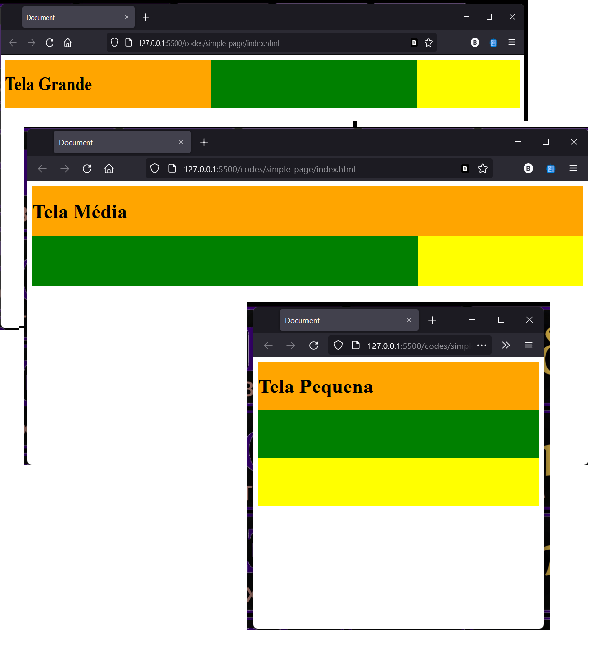
\includegraphics[scale=0.6]{14-layout-flex.png}
	\caption{Layout Flex com Media Queries}
\end{figure}

\textbf{Layout Grid}
\\~\\
Para além das medias queries e layout flex, podemos construir o front end de uma aplicação usando o Sistema Grid que o CSS possui. A ideia é pensar no front end da aplicação em termos de dois elementos visuais: O Container e os Itens.
\\~\\
\textbf{Comentário:} Depois eu vou revisitar essa seção com base no material disponível nesse \href{https://css-tricks.com/snippets/css/complete-guide-grid/}{[link]}.
\\~\\
O sistema Grid possui alguns conceitos que nos ajudam a criar e manter a interface de uma aplicação que use essa metodologia:
\begin{itemize}
	\item Line - Separa as cells
	\item Cell - É uma unidade encapsulada em uma linha e uma coluna
	\item Area - Conjunto de cells
	\item Track - Um conjunto linear de cells (uma linha ou uma coluna do grid)
\end{itemize}

Abaixo temos o código de uma aplicação simples usando esse sistema de construção de front end:

\scriptsize
\begin{Verbatim}[tabsize=4,frame=single]
 ------- Parte HTML -------
<body>
    <div class="container">
        <header>Header </header>
        <main>Main</main>
        <nav>Sidebar</nav>
        <footer>Footer</footer>
    </div>
</body>

------- Parte CSS -------
body {
    background-color: rgb(255, 255, 255);
}

.container {
    height: 700px;
    display: grid;
    grid-template-columns: 20% 30% 30% 19%;
    grid-template-rows: auto;
    grid-template-areas:
    "header header header header"
    "main main main sidebar"
    "footer footer footer footer";
    column-gap: 5px;
    row-gap: 5px;
}

header {
    grid-area: header;
    background-color: orange;
    height: 100px;
}

main {
    grid-area: main;
    background-color: blue;
    height: 500px;
}

nav {
    grid-area: sidebar;
    background-color: red;
    height: 500px;
}

footer {
    grid-area: footer;
    background-color: green;
    margin: solid black 5px;
    height: 100px;
}
\end{Verbatim}
\normalsize

\begin{figure}[H]
	\centering
	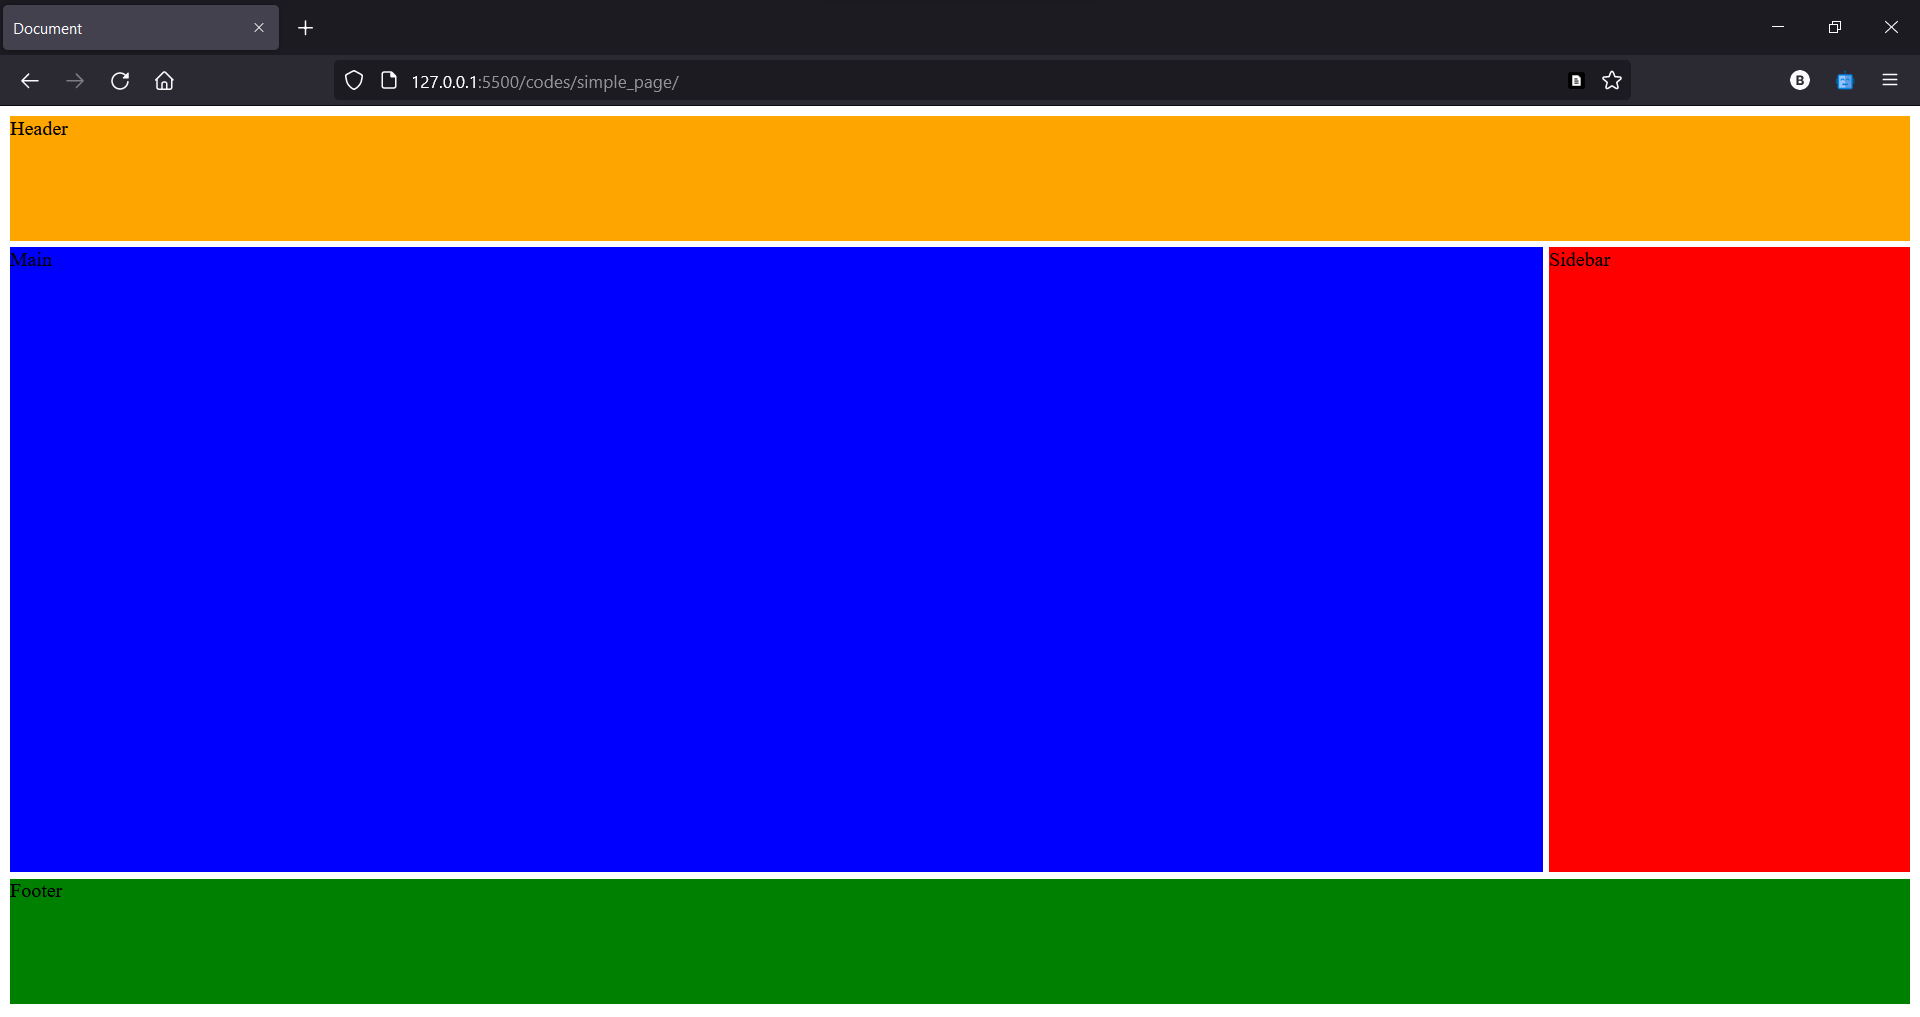
\includegraphics[scale=0.3]{15-layout-grid.png}
	\caption{Layout Grid}
\end{figure}

Com base nessa lógica, podemos posicionar elementos usando o sistemas de coordenadas do CSS Grid. Vamos refazer a interface que acabamos de ver usando apenas esse conceito de ``items'' dentro de um ``container''.
\\~\\
Ao invés de definir a separação da tela como parâmetro da classe container no CSS, nós vamos criar o container e orientar, dentro de cada item, como ele se comportará no grid.

\scriptsize
\begin{Verbatim}[tabsize=4,frame=single]
------ Parte HTML ------
<body>
    <div class="container">
        <div class="item-a">Header</div>
        <div class="item-b">Main</div>
        <div class="item-c">Nav</div>
        <div class="item-d">Footer</div>
    </div>
</body>

------ Parte CSS ------
body {
    background-color: rgb(255, 255, 255);
}

.container {
    height: 700px;
    display: grid;
    grid-template-columns: 24% 25% 25% 25%;
    grid-template-rows: 10% 80% 10%;
    grid-column-gap: 5px;
    grid-row-gap: 5px;
}

.item-a {
    background-color: orange;
    grid-column-start: 1;
    grid-column-end: span 4;
    grid-row-start: 1;
    grid-row-end: 1;
}

.item-b {
    background-color: blue;
    grid-column-start: 1;
    grid-column-end: span 3;
    grid-row-start: 2;
    grid-row-end: 2;
}

.item-c {
    background-color: red;
    grid-column-start: 4;
    grid-column-end: 4;
    grid-row-start: 2;
    grid-row-end: 2;
}

.item-d {
    background-color: green;
    grid-column-start: 1;
    grid-column-end: span 4;
    grid-row-start: 3;
    grid-row-end: 3;
}
\end{Verbatim}
\normalsize

Nem vale a pena mostrar uma imagem do resultado porque ele é exatamente igual à imagem anterior.
\\~\\
Com isso, podemos ver que é o desenvolvimento de uma interface de aplicação web pode ser feito de diferentes maneiras, mas o que realmente importa é uma boa documentação e um planejamento bem feito para que o cliente termine com o que ele realmente precisa e o time de desenvolvimento não precise perder preciosas horas no bem conhecido ciclo de ``vai-e-volta'' até que o cliente aceite algum layout.
\\~\\
\textbf{Exemplo de Aplicação Web Responsiva}
\\~\\
Para finalizar nosso estudo de desenvolvimento web com CSS vamos fazer uma aplicação simples. O protótipo no MarvelApp pode ser visto nesse \href{https://marvelapp.com/prototype/i4hhafb/screen/86385696}{[link]}.
\\~\\
O código que gerou esse resultado pode ser visto no repositório desse projeto nesse \href{https://github.com/brunoruas2/Analise_Des_Sistemas/tree/main/Book/codes/dev_web_css}{[link]}.

\begin{figure}[H]
	\centering
	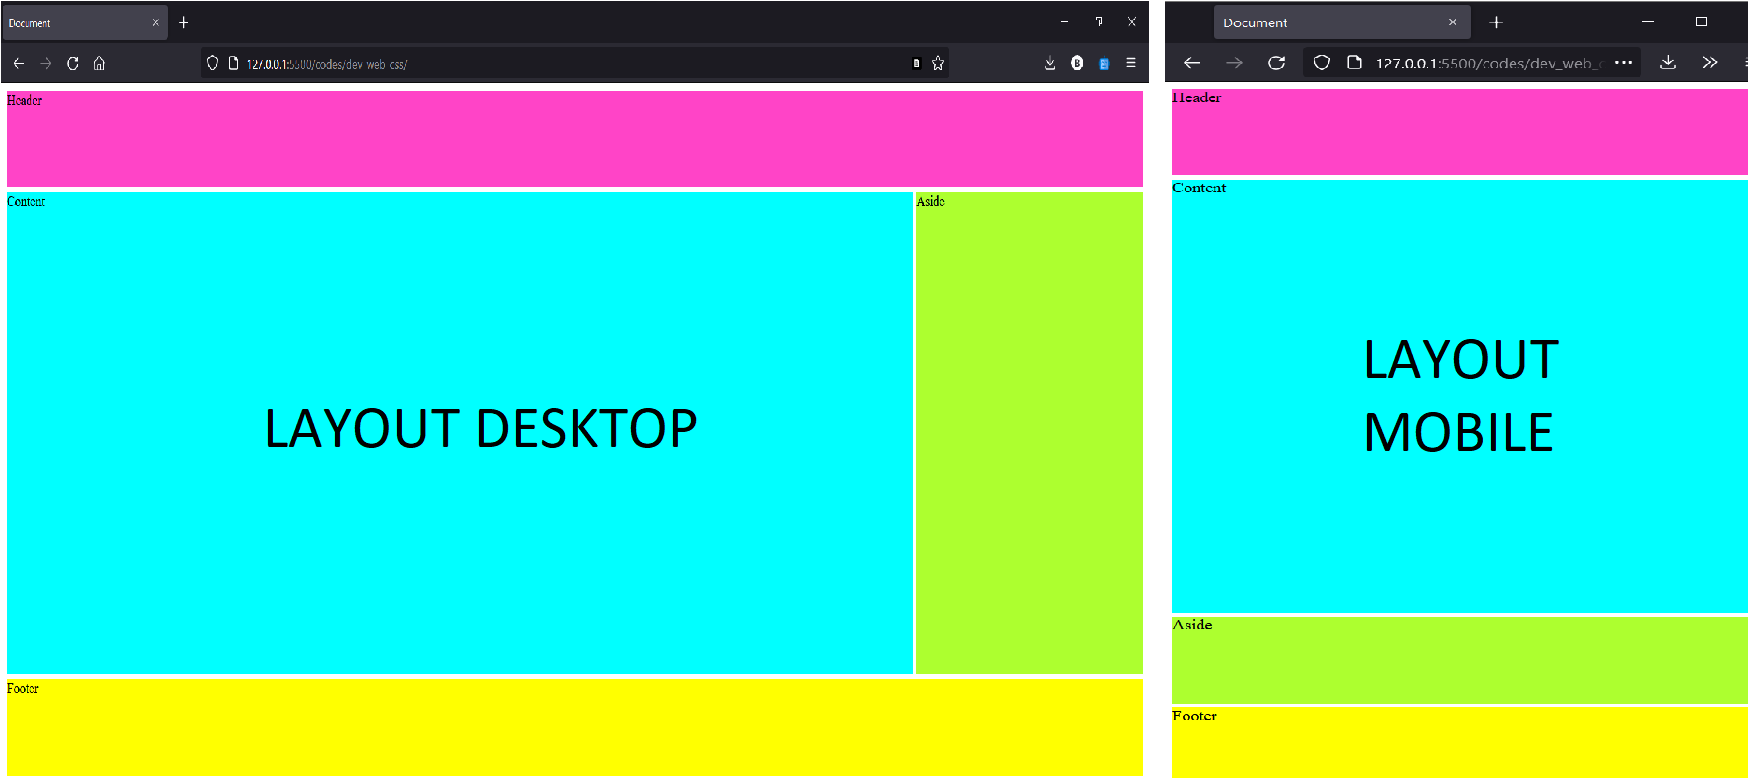
\includegraphics[scale=0.3]{16-responsividade-front-end.png}
	\caption{Aplicação com front end responsivo}
\end{figure}

\textbf{Comentário:} Acredite, com os conceitos aprendidos até agora nós já conseguimos fazer aplicações simples com páginas estáticas com relativa facilidade. Uma disso é que enquanto escrevo esse parágrafo\footnote{Dia 29/04/2022.} eu acabei de criar a primeira página da aplicação web front end que meu grupo precisa entregar como projeto do primeiro semestre da graduação. Eu usei, basicamente, apenas o que aprendemos aqui e alguma pesquisa no google para coisas mais simples.

\begin{figure}[H]
	\centering
	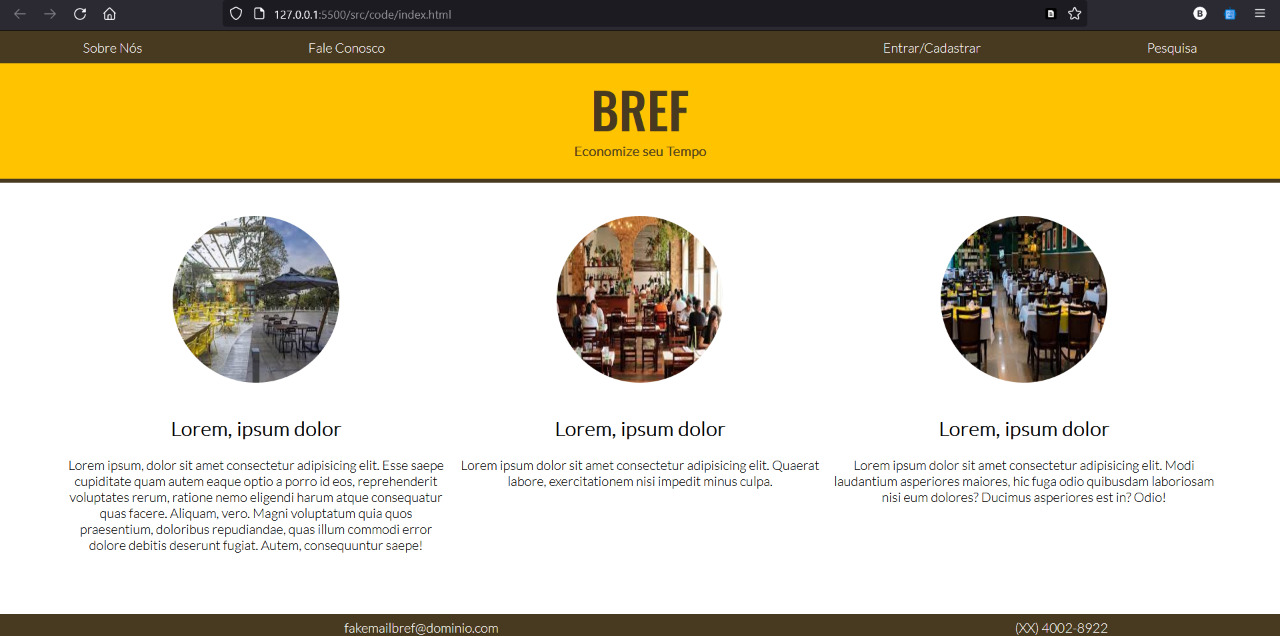
\includegraphics[scale=0.25]{17-brefV1.jpg}
	\caption{Página inicial usando o sistema grid e viewport.}
\end{figure}


\subsubsection{Frameworks front-end - Bootstrap}

Como era de se esperar, os programadores perceberam que era possível combinar várias práticas do mercado em ``pacotes'',``bibliotecas'' ou ``frameworks'' que, no fundo, são códigos escritos em HTML, CSS e JavaScript. Essas ferramentas facilitam demais o processo de desenvolvimento mas, como tudo na vida, precisam ser usadas com moderação e habilidade. Não podemos correr o risco de virarmos ``escravos'' de nenhum framework.
\\~\\
Com o devido aviso dado, podemos iniciar nosso estudo de Frameworks famosos com o \href{Bootstrap}{Boostrap}. A culpa de várias sites que acessamos terem um ``jeitão'' parecido é, em boa parte, desse framework que até hoje é o mais famoso. Foi desenvolvido em 2011 por Mark Otto e Jacob Thornton no Twitter\footnote{Isso mesmo.} e disponibilizado no GitHub.
\\~\\
O Bootstrap se ajusta automaticamente a diferentes modelos de tela porque tem, dentro dele, tamanhos pré-determinados de telas que se ajustam ao dispositivo\footnote{Igual a nossa aplicação usando viewport.}. A ``fronteira'' entre os tamanhos de tela são os chamados \textbf{Breakpoints}. A tabela abaixo resume as relações entre tamanho da tela e ajuste do container da aplicação. O site oficial pode ser acessado nesse \href{http://getbootstrap.com/}{[link]}.

\begin{center}
\scriptsize
\begin{tabular}{|c|c|c|c|c|c|}
	\hline
	& \textbf{Extra Small} & \textbf{Small} & \textbf{Medium} & \textbf{Large} & \textbf{Extra Large}  \\
	& <57px & $\geq$ 576px & $\geq$ 768px & $\geq$ 992px & $\geq$ 1200px \\ 
	\hline
	\hline
	Max container size & (auto) & 540px & 720px & 960px & 1140px \\
	\hline
	Nome da Classe & \verb|.col-| & \verb|.col-sm-| & \verb|.col-md-| & \verb|.col-lg-| & \verb|.col-xl-| \\
	\hline

\end{tabular}
\normalsize
\end{center}
\ 
\\~\\
\textbf{Download do Bootstrap}
\\~\\
Existem duas opções de download desse Framework:
\begin{itemize}
	\item CSS e JS compilados - Já vem pronto pra uso mas é um pouco limitado.
	\item Código Fonte - Permite customização e vem com as fontes do Bootstrap mas precisa de compilação.
\end{itemize}

Para saber como fazer basta uma pesquisa rápida no \href{https://www.google.com/search?channel=crow5&client=firefox-b-d&q=como+instalar+o+boostrap}{[google]} ou no \href{https://www.youtube.com/results?search_query=how+to+install+and+use+boostrap}{[youtube]}.
\\~\\
\textbf{Conteúdo do Boostrap}
\\~\\
A melhor fonte sobre qualquer tecnologia geralmente é a própria \href{https://getbootstrap.com/docs/5.1/getting-started/introduction/}{documentação oficial}. Mas podemos dividir as partes do Bootstrap em:
\begin{itemize}
	\item Reboot - Para uniformização da aparência em diferentes navegadores
	\item Tipografia - Textos e fontes
	\item Code - Linhas de código
	\item Images - Relacionado aos recursos de imagens
	\item Tables - Relacionado aos recursos de tabelas
	\item Figures - Imagens com textos associados
\end{itemize}
\ 
\\~\\
\textbf{Componentes do Boostrap}
\\~\\
Nós já sabemos que o HTML possui uma lógica de estruturação da página. Contudo, quando estamos usando o Bootstrap temos que ``reaprender'' como pensar nossa estrutura da página a partir dos conceitos e modelos do framework.
\\~\\
Para o Bootstrap, a página é criada usando-se \textbf{componentes}. A lista é bem grande mas podemos destacar alguns:
\begin{itemize}
	\item Breadcrumb - Trilha com o caminho do site até uma página
	\item Navbar - Barra de menu e pesquisa
	\item Carousel - Conjunto rotativo de imagens em destaque no site
	\item Cards - Cartões para uso diverso. Podem ser imagens ou texto
	\item Modal - Caixas de diálogo (tipo um popup só que dentro da página)
\end{itemize}
\ 
\\~\\
\textbf{Sistema Grid no Bootstrap}
\\~\\
Como nós já sabemos, o sistema grid é uma maneira conveniente de controlarmos a estrutura visual da nossa aplicação. Diante disso, não é surpreendente que esse framework também use uma versão dessa lógica.
\\~\\
Para o Bootstrap, \textbf{todas as páginas} serão sempre divididas em 12 colunas. Quando um elemento está dentro de outro, o padrão de 12 colunas se mantém. A lógica de divisão é como na imagem abaixo:

\begin{figure}[H]
	\centering
	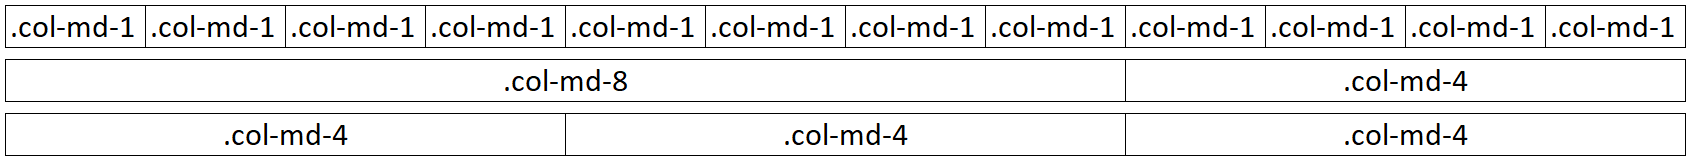
\includegraphics[scale=0.35]{17-boostrap-columns.png}
	\caption{Colunas no Bootstrap}
\end{figure}

O código HTML usando o Bootstrap é fortemente baseado em \verb|<div>|. A novidade está no uso de classes específicas que dão a lógica contida nos arquivos usados pelo framework.
\\~\\
A hierarquia é similar ao grid system porque a aplicação existira dentro de um container. O Container terá pelo menos uma linha (row). Cada linha terá pelo menos uma coluna. Internalize essa hierarquia de Container, Linhas e Colunas.

\scriptsize
\begin{Verbatim}[frame=single,tabsize=4]
----- HTML -----
<div class="row">
	<div class="col-md-6" id="cel1">.col-md-6</div>
	<div class="col-md-6" id="cel2">.col-md-6</div>
</div>
<div class="row">
	<div class="col-md-2" id="cel1">.col-md-2</div>
	<div class="col-md-10" id="cel2">.col-md-10</div>
</div>
<div class="row">
	<div class="col-md-9" id="cel1">.col-md-9</div>
	<div class="col-md-3" id="cel2">.col-md-3</div>
</div>

----- CSS ------
#cel1 {
    color: white;
    background-color: red;
    height: 100px;
    border: solid black 3px;
}

#cel2 {
    color: white;
    background-color: blue;
    height: 100px;
    border: solid black 3px;
}
\end{Verbatim}
\normalsize

Na próxima imagem podemos ver o resultado desse código. O sistema de 12 colunas md-1 torna bem simples a disposição dos conteúdos na tela.

\begin{figure}[H]
	\centering
	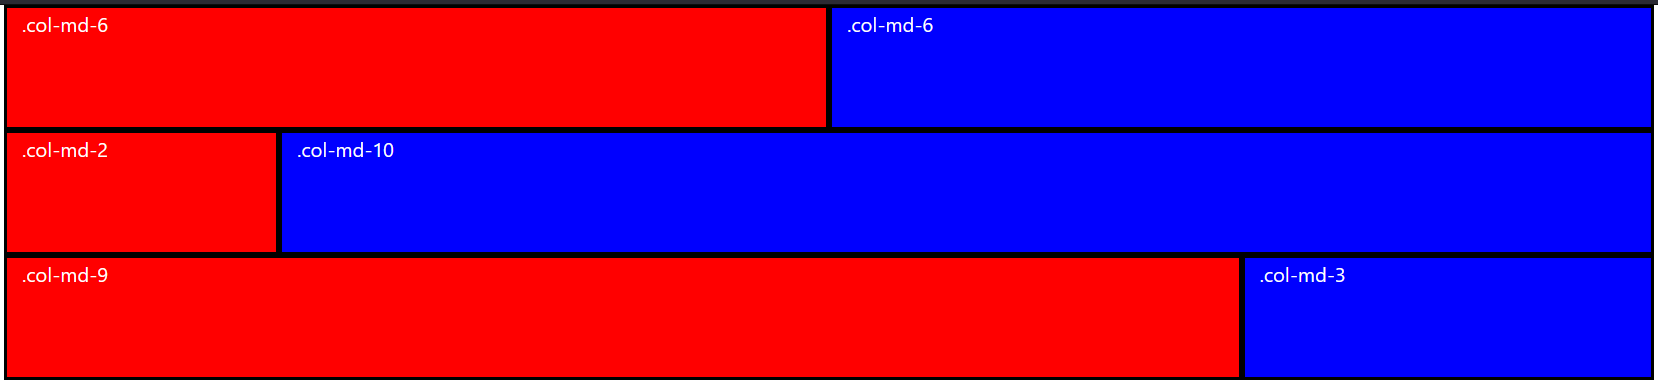
\includegraphics[scale=0.35]{18-bootstrap-columnsrows}
	\caption{Container, Rows e Columns}
\end{figure}

\textbf{Exercício Prático - Site de Wired usando Bootstrap}
\\~\\
Para exercitar esses conceitos, podemos usar como referência a página do famoso site de notícias Wired\footnote{Acesso em 02/05/2022.}. A imagem de referência será a versão desktop e a mobile do site.

\begin{figure}[H]
	\centering
	
\includegraphics[scale=0.25]{19-desafio-wired.png}
	\caption{Layout Desktop e Mobile}
\end{figure}

A primeira coisa que precisamos é identificar as estruturas de linhas e colunas da visão desktop. Podemos ver que temos uma barra superior. Uma estrutura de 3 colunas sendo as duas primeiras referentes à uma seção e a lateral direita referente a outra seção.
\\~\\
Em termos dos componentes do bootstrap, podemos fazer uma interface equivalente como na imagem abaixo.
\\~\\
\textbf{Comentário:} Eu to com prazo curto agora por causa do cronograma das aulas então vou ter que deixar esse desafio para depois.

\subsection{A Linguagem JavaScript}

Já aprendemos que a Web utiliza a linguagem HTML para estrutura do conteúdo, a linguagem CSS para formato e apresentação. Contudo, nós sabemos que hoje em dia as aplicações possuem funções bem complexas com sistemas inteiros baseados todo no navegador do client. A linguagem JavaScript é justamente o mecanismo que trás essa capacidade de interatividade e processamento para à web.
\\~\\
Hoje em dia, a linguagem JavaScript (também chamada de JS) é mantida pela \href{https://www.ecma-international.org/mission/}{ECMA International}. Uma organização suíça criada em 1961 cujas atividades são separadas em vários campos de atuação. Um desses campos é a padronização de linguagens de programação. Atualmente, ela elabora os padrões para as linguagens ECMAScript (TC39), C\# (TC49) e outras.
\\~\\
Sim, é isso mesmo. Nada de JavaScript. O JS foi criado em 1995 por Brendan Eich mas em 1996 foi transferido para a ECMA para padronização. O primeiro padrão JS dentro do ECMAScript foi feito em 1997.
\\~\\
Como consta na edição 2020 do padrão ``O ECMAScript é baseado em várias tecnologias cujas mais conhecidas são o JavaScript (Netscape) e JScript (Microsoft)''. O ECMAScript foi adotado na maioria dos navegadores desde o final dos anos 90. Hoje em dia, praticamente todos os navegadores adotam o padrão ECMAScript e, consequentemente, o JavaScript dentro deles.
\\~\\
A ECMA International cria os padrões e especificações que permitam a execução de uma determinada linguagem. O JS é a implementação dessas padronizações dentro dos navegadores do mercado. Tanto é assim, que diferentemente do que acontece com as outras linguagens como Python, R e etc, você não precisa instalar um interpretador ou um compilador para rodar códigos em JS. Os navegadores possuem, dentro deles, um motor próprio que executa o padrão ECMAScript.
\\~\\
Para citar alguns desses motores:
\begin{center}
\begin{tabular}{|c|c|c|}
	\hline
	\textbf{Navegador} & \textbf{Motor Web} & \textbf{Motor ECMAScript} \\
	\hline
	\hline
	Firefox & Gecko & Spider Monkey \\
	\hline
	Chrome & Blink & Google V8 \\
	\hline
	Safari & WebKit & JavaScriptCore \\
	\hline
	IE & Trident & Chakra Core \\
	\hline
	Edge & EDGE & Chakra Core \\
	\hline
	Opera & Blink & \\
	\hline
\end{tabular}
\end{center}

\textbf{Comentário:} Não confunda a linguagem de programação \href{https://www.java.com/pt-BR/}{Java} com JavaScript. São linguagens totalmente diferentes.
\\~\\
\textbf{Aplicação da Linguagem JavaScript}
\\~\\
Da mesma maneira que vimos com o CSS, podemos trazer o JS para nossa aplicação web de diferentes maneiras:
\begin{itemize}
	\item Por arquivo externo - Código é mantido em um arquivo separado
\begin{Verbatim}
<script type="text/javascript" src="script.js"></script>
\end{Verbatim}
	\item Em Bloco interno - Código fica em um bloco dentro do HTML
\begin{Verbatim}
<script type="text/javascript">
	/* Código JS */
	alert("Olá mundo!");
</script>
\end{Verbatim}
	\item Inline - Código fica dentro de um atributo do elemento HTML
\begin{Verbatim}
<p onClick="alert("Click feito!");"></p>
\end{Verbatim}
\end{itemize}

Agora que sabemos que podemos ``turbinar'' nossas páginas web com o uso de JS, podemos nos perguntar o que pode ser feito com essa ferramenta. A resposta é praticamente qualquer coisa! Podemos elencar como principais aplicações:
\begin{itemize}
	\item Manipulação de objetos e tratamento de eventos relacionados aos elementos HTML a partir do uso de uma API chamada DOM (Documento Object Model)\footnote{Sério, dá pra gerar praticamente uma página HTML com o uso do DOM. Isso é muito poderoso.}
	\item Comunicação com servidores e utilização de APIs via AJAX\footnote{Veremos mais pra frente o que é isso.} usando o XMLHttpRequest ou na API Fetch
	\item Armazenamento de dados no client com o uso das APIs Indexed DB e LocalStorage/SessionStorage
	\item Usar as APIs do HTML5: Canvas, Media, File, Drag and Drop, Geolocation, Web Workers, History
\end{itemize}
\ 
\\~\\
\textbf{JavaScript além do Browser}
\\~\\
As pessoas gostaram tanto de JS que foram capazes de construir uma aplicação que implementa o v8 do chrome fora do browser. Isso mesmo, podemos rodar aplicações em JS direto no terminal do seu computador. Basta usar a aplicação \href{https://nodejs.org/en/}{Node.js}. Hoje em dia, dá pra fazer uma aplicação inteira, backend e frontend com JS.
\\~\\
Com JS podemos também construir aplicações desktop usando uma biblioteca chamada \href{https://www.electronjs.org/}{Electron}.
\\~\\
Esse aqui é apenas o começo da nossa caminhada!

\subsubsection{Variáveis e Tipos de Dados}

A linguagem JS é de tipagem dinâmica. Então o tipo de variável é definido pela própria linguagem na hora da atribuição do valor. Temos dois tokens de atribuição em JS \textbf{var} ou \textbf{let}.

\begin{Verbatim}[tabsize=4,frame=single]
var variavel01;     // Aqui eu declarei sem atribuir nada
var x = 10;         // x agora é um numérico de valor 10
let y = "Olá mundo" // y é uma string
\end{Verbatim}

Agora temos que entender o motivo de termos dois tokens de atribuição. Mas, para poder explicar isso, precisamos entender que existem diferentes \textbf{escopos de variáveis} quando um programa em JS é executado. Os escopos das variáveis em JS são:
\begin{itemize}
	\item Escopo Global - Variáveis sempre disponíveis para consulta e edição
	\item Escopo Local - Variáveis existem apenas dentro de um bloco de código (um loop ou uma condicional, por exemplo)
\end{itemize}

As variáveis declaradas com \verb|var| são de \textbf{escopo global} se forem declaradas fora de funções\footnote{Nesse caso são de escopo local}. Já a atribuição feita com \verb|let| é de \textbf{escopo local}.
\\~\\
Abaixo temos um exemplo bem bacana mostrando essas diferenças.

\begin{Verbatim}[tabsize=4,frame=single]
var a = 5;
var b = 10;

if (a === 5) {
	let a = 4;
	var b = 1;

	console.log(a);
	console.log(b);
}

-> Mostra 4 e 1 no console

console.log(a);
console.log(b);

-> Mostra 5 e 1 no console
\end{Verbatim}

\textbf{Comentário:} Uma boa prática em JS (e em praticamente todas as linguagens) é sempre declarar as variáveis na parte de cima de cada bloco ou no começo do código.
\\~\\
Também é possível usar o token \verb|const| para atribuição. Esse token funciona igual ao \verb|let| e é definido para constantes. Uma boa prática da comunidade é usar letra maiúsculas para definir suas constantes.
\\~\\
\textbf{Tipos e Estruturas de Dados}
\\~\\
Todas as variáveis que são números, textos (strings) ou valores booleanos (true ou false) são o que chamamos de \textbf{tipo Primitivo}. As variáveis especiais do tipo nulo (null) ou indefinido (undefined) são possuem características de tipo primitivo mas podem ser entendidas como sendo de um tipo único especial. No ECMAScript 6 foi inserida uma nova categoria de variáveis chamadas de \textbf{tipo Simbólico ou Symbol}\footnote{Não vamos nos aprofundar nisso agora. Depois eu atualizo esse material com o ECMAScript 6.}. O que não for de tipo primitivo, null, undefined ou symbol, será do \textbf{tipo Objeto} que possui uma lista de propriedades, que por sua vez, possuem um nome e valores associados.
\\~\\
Podemos resumir o que acabamos de ver como:
\begin{figure}[H]
	\centering
	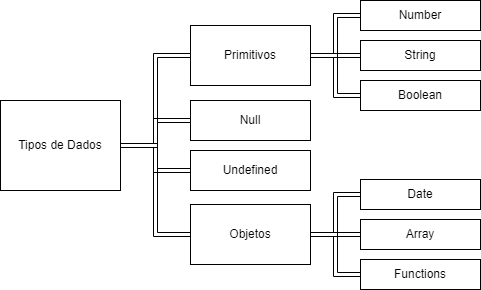
\includegraphics[scale=0.8]{20-tipos-var-JS.png}
	\caption{Tipos de Dados do JavaScript}
\end{figure}

\textbf{Tipo Numérico}
\\~\\
JS não faz diferença entre números inteiros ou fracionados. Para essa linguagem, tudo é considerado o que chamamos de \textbf{ponto flutuante} de 64 bits. O valor máximo possível é acessado pela propriedade do objeto \verb|Number| por meio das propriedades \small \verb|Number.POSITIVE_INFINITY| e \verb|Number.NEGATIVE_INFINITY|\normalsize.
\\~\\
Quando tentamos fazer uma operação matemática não possível (como raiz de -1) recebemos o resultado \verb|NaN| que significa Not-a-Number.
\\~\\
Não é incomum termos que converter caracteres do tipo texto mas que representam números. Para isso, podemos usar a função nativa \verb|parseInt| ou \verb|parseFloat|.
\\~\\
\textbf{Tipo Boolean}
\\~\\
Os operadores booleanos são operadores que apenas admitem duas entradas: \verb|true| ou \verb|false|. Podemos chamar essas entradas diretamente ou através de operações lógicas usando operadores lógicos ou matemáticos. Abaixo temos uma tabela que podemos usar de referência.

\begin{center}
\begin{tabular}{|l|c|l|}
	\hline
	\textbf{Operador} & \textbf{Exemplo} & \textbf{Observação} \\
	\hline
	\hline
	Mesmo valor & x == y & true se mesmo valor \\
	\hline
	Mesmo valor e tipo & x === y & true se mesmo valor e tipo \\
	\hline
	Diferente valor & x !== y & true se diferente valor \\
	\hline
	Maior que & x > y & true se x maior que y \\
	\hline
	Menor que & x < y & true se x menor que y \\
	\hline
	Maior igual & x >= y & true se maior igual \\
	\hline
	Menor igual & x <= y & true se menor igual \\
	\hline
	Negação & !x & true se x for false \\
	\hline
	And & x \&\& y & true se x e y forem true \\
	\hline
	Or & x || y & true se x ou y forem true \\
	\hline
\end{tabular}
\end{center}
\ 
\\~\\
\textbf{Tipo String}
\\~\\
Qualquer aplicação precisa ser capaz de lidar com textos. Uma string é exatamente uma cadeia de caracteres não numéricos (mas caracteres numéricos também podem compor uma string) que pode ser declarada por meio de aspas simples ``abc'' ou compostas `abc'.
\\~\\
Também é comum precisarmos juntar diferentes strings. No javascript, podemos fazer isso simplesmente usando o operador de soma:

\begin{Verbatim}[tabsize=4,frame=single]
str = `abc' + `def'

console.log(str)

-> abcdef
\end{Verbatim}

Alguns caracteres das nossas strings podem ser os mesmos usados na própria linguagem. Isso nos obriga a termos que aprender como fazer um ``bypass'' desses caracteres. Abaixo temos uma tabela para referência.

\begin{center}
\begin{tabular}{|l|l|}
	\hline
	\textbf{Código} & \textbf{Significado} \\
	\hline
	\hline
	$\backslash$0 & Null \\
	\hline
	$\backslash$' & Aspas simples \\
	\hline
	$\backslash$" & Aspas compostas \\
	\hline
	$\backslash \backslash$ & Barra invertida \\
	\hline
	$\backslash$n & Nova linha \\
	\hline
	$\backslash$r & Retorno \\
	\hline
	$\backslash$v & Tabulação Vertical \\
	\hline
	$\backslash$t & Tabulação \\
	\hline
	$\backslash$b & Backspace \\
	\hline
	$\backslash$f & form feed \\
	\hline
	$\backslash$uXXXX & Unicode \\
	\hline
	$\backslash$xXX & Latin-1 \\
	\hline
\end{tabular}
\end{center}

A partir do ECMAScript6 existe outra maneira de compor strings: por meio do uso da crase \verb|`isso é uma string`|. A vantagem desse método, chamado de \textbf{TemplateString} é que esse tipo de string é especial que pode receber expressões interpretáveis como no exemplo abaixo:

\begin{center}
\begin{Verbatim}[tabsize=4,frame=single]
nome = "bruno"
console.log(nome)
-> bruno

linha = `meu nome é ${nome}`
console.log(linha)
-> meu nome é bruno
\end{Verbatim}
\end{center}

Podemos ver que na última linha o resultado faz uso do valor da variável \verb|nome|. Provavelmente, sempre que a gente entra em um site que possui aquela mensagem amigável de ``Seja bem vindo, Fulano'', o programador usou essa função para produzir aquele texto.
\\~\\
\textbf{Tipo Objeto}
\\~\\
Objetos são uma boa parte do que faz o JS ser tão poderoso. Cada objeto é simplesmente uma coleção de pares nome-valor. Os nomes são as \textbf{propriedades} do objeto e os valores podem ser qualquer tipo de variável que vimos logo antes (incluindo outros objetos e funções). Quando a propriedade for uma função, dizemos que essa função é um \textbf{método} do objeto.

\begin{Verbatim}[tabsize=4,frame=single]
var objeto1 = new Object(); // Criando o objeto "objeto1"

objeto1.name = "bruno"; // modo 1 de criar uma propriedade
objeto1["age"] = 28;    // modo 2 de criar uma propriedade

console.log(objeto1)
-> { age:28 , name:bruno }

var objeto2 = {         // modo de criar o objeto 
	nome: "bruno",		// junto das propriedades
	idade: 28
}
console.log(objeto2)
-> { nome:bruno, idade: 28 }
\end{Verbatim}

Para acessar o valor de uma propriedade em um objeto basta escrever algo como: \verb|objeto.propriedade|.\footnote{Python é assim também.}
\ 
\\~\\
\textbf{Datas e Horas}
\\~\\
Na elaboração de uma aplicação é comum ter que lidar com varáveis do relacionadas ao tempo. Para isso o JS possui um tipo de objeto especialmente projetado para facilitar essa tratativa. O objeto \verb|Date()|. Podemos usa-lo como:

\begin{center}
\begin{Verbatim}[tabsize=4,frame=single]
var a = new Date() // Atribui a data atual ao objeto
var c = new Date(string) // Atribui a data por uma string
var d = new Date(Ano,Mes,Dia,Hora,Segundo,Milisegundos)
\end{Verbatim}
\end{center}

Geralmente estamos preocupados apenas com o dia, mês e ano. Para criar um objeto com esses valores basta ir colocando na mesma ordem do último elemento do exemplo acima.
\\~\\
\textbf{Aviso:} Quando você for indicar o mês, saiba que para o JS, janeiro é 0 e dezembro é 11. Então quando quisermos salvar a data `01/01/2022' usaremos \verb|Date(2022,0,1)|.
\\~\\
Como todo objeto, a variável criada com o Date() possui várias propriedades e métodos. Uma boa referência é o material do MDN que pode ser visto \href{https://developer.mozilla.org/en-US/docs/Web/JavaScript/Reference/Global_Objects/Date}{[aqui]}. Mas podemos elencar alguns médodos importantes como:

\begin{center}
\begin{Verbatim}[tabsize=4,frame=single]
var z = new Date()

z.getFullYear()
z.getMonth()
z.getDate()
z.getDay()
z.getHours()
z.getMinutes()
z.getSeconds()
z.getMillisecondes()
z.getTimes()
\end{Verbatim}
\end{center}

Acho que não é necessário explicar cada método desse porque o nome é bem alto explicativo.
\ 
\\~\\
\textbf{Arrays, Vetores ou Matrizes}
\\~\\
Um array é uma estrutura de dados semelhante a uma lista. Em JS temos algumas maneiras de criar arrays:

\begin{center}
\begin{Verbatim}[tabsize=4,frame=single]
/* Modo 01 */
var a = new Array()
a[0] = 'valor01'
a[1] = 'valor02'

/* Modo 02 */
var b = new Array('valor01','valor02')

/* Modo 03 */
var c = ['valor01','valor02']
\end{Verbatim}
\end{center}

Todos os 3 modos produzem o mesmo resultado e podem ser usados alternadamente.
\\~\\
Como qualquer objeto, existem vários métodos muito úteis dentro de um Array().

\scriptsize
\begin{center}
\begin{Verbatim}[tabsize=4,frame=single]
concat() // Junta dois ou mais vetores
fill() // Preencher os elementos em um vetor com um valor estático
find() // Retorna o valor do primeiro elemento em um vetor que atender ao filtro
findIndex() // Retorna o índice do primeiro elemento em um vetor
forEach() // Chama uma função para cada elemento do vetor
indexOf() // Busca um elemento no vetor e retorna a sua posição
isArray() // Verifica se um objeto é um vetor
join() // Junta todos os elementos de um vetor em uma string
lastIndexOf() // Pesquisar o vetor por um elemento, começando no final
pop() // Remove o último elemento de um vetor e retorna o elemento
push() // Adiciona novos elementos para o final de um vetor
reverse() // Inverte a ordem dos elementos em um vetor
slice() // Seleciona uma parte de um vetor e retorna o novo vetor
sort() // Classifica os elementos de um vetor
splice() // Adiciona/remove elementos de um vetor
toString() // Converte um vetor em uma string e retorna o resultado
valueOf() // Retorna o valor primitivo de um vetor
\end{Verbatim}
\end{center}
\normalsize

\textbf{Comentário:} Eu achei estranho que o material não falou nada sobre vetor e matriz. Então uma hora eu volto para expandir essa parte com esses outros dois tipos de dados.

\subsubsection{Controle de Fluxo}

Em qualquer linguagem de programação\footnote{Sempre vai existir alguma excessão, eu sei.} existem maneiras de organizar blocos de código para o compilador/interpretador saber o que priorizar na hora do processamento do código. Em JS isso é feito com o uso das chaves \{ \}.
\\~\\
\textbf{Declarações de Seleção}
\\~\\
Quando estamos fazendo um script de código, é muito comum termos que nos adaptar as situações onde determinados eventos podem ou não acontecer. Para isso, usamos algumas estruturas lógicas que permitem o processamento de blocos de texto apenas se alguma condição predeterminada seja satisfeita. Ou seja, usamos um condicionante do tipo ``Se-Então''.

\begin{center}
\begin{Verbatim}[tabsize=4,frame=single]
if (expressao) {
	bloco de codigo caso true
}
else {
	outro bloco de codigo caso false
}
\end{Verbatim}
\end{center}

Existem situações onde existem múltiplas possibilidades. Pensando nisso, o JS possui um operador de \verb|switch| que permite vários condicionantes de maneiras mais simples do que vários \verb|if|s sucessivos.

\begin{center}
\begin{Verbatim}[tabsize=4,frame=single]
switch (expressao) {
	case valor01:
	bloco_se_01
	break

	case valor02:
	bloco_se_02
	break

	default:
	bloco_se_nao_01_ou_02
	break
}
\end{Verbatim}
\end{center}

Veja que usamos o token \verb|break| para indicar que vamos para outra condicional. Não podemos esquecer disso.
\\~\\
Abaixo temos um exemplo de uma aplicação simples usando esse método de gestão de fluxo. Não se preocupe em entender o código inteiro, foque apenas no que estamos estudando.

\begin{center}
\begin{Verbatim}[tabsize=4,frame=single]
// Função que recebe um input no terminal
const readLine = require('readline').createInterface({
	input: process.stdin,
	output: process.stdout
})

readLine.question('Qual seu nome? ', name => {
	switch (name) {
		case 'bruno':
			console.log(`OI, BRUNO!`)
			break
	
		case 'mario':
			console.log('Salve, Mario!')
			break
		
		default:
			console.log(`Olá, ${name}. Seja bem-vindo(a)!`)
	}
	readLine.close()
})

> Qual seu nome? bruno
> OI, BRUNO!

> Qual seu nome? mario
> Salve, Mario!

> Qual seu nome? pedro
> Olá, pedro. Seja bem-vindo(a)!
\end{Verbatim}
\end{center}

\textbf{Declarações de Repetição}
\\~\\
Além de termos tokens que nos permitem executar apenas alguns blocos de código. Existem outros que nos permitem usarmos um mesmo bloco de código repetidamente. Chamamos essas estruturas lógicas de laços de repetição.
\\~\\
A primeira maneira de criarmos um laço de repetição em JS é por meio do token \verb|while| do seguinte modo:
\begin{center}
\begin{Verbatim}[tabsize=4,frame=single]
// Exemplo de loop com while
var i = 0

while (i <= 5) {
	console.log(`Contagem: ${i}`)
	i++ // soma + 1 ao valor de i
}

> Contagem: 0
> Contagem: 1
> Contagem: 2
> Contagem: 3
> Contagem: 4
> Contagem: 5
\end{Verbatim}
\end{center}

Primeiro criamos a variável \verb|i| e usamos a estrutura de loop \verb|while| para a seguinte regra ``Se i for menor igual a 5 então mostre a mensagem `Contagem: Número i'''. Quando o valor da variável \verb|i| é 6, a expressão do loop retorna um false e saímos do loop.
\\~\\
O operador que aprendemos anteriormente faz um loop enquanto a condição expressa entre os parênteses não for false. Mas existem situações onde queremos executar o bloco de código um número definido de vezes. Para isso o JS possui o token \verb|for|.

\begin{center}
\begin{Verbatim}[tabsize=4,frame=single]
// Exemplo de loop com for
let frutas = ['pera','uva','maca','banana']

for (let index = 0; index < frutas.length; index++) {
	console.log(frutas[index])
}

> pera
> uva
> maca
> banana
\end{Verbatim}
\end{center}

Nesse exemplo acima vemos que o parênteses da expressão do \verb|for| possui 3 linhas de códigos separadas por ponto e vírgula. Na primeira, criamos uma variável index. Na segunda, temos a nossa expressão que avalia se o index é menor que o tamanho do array frutas. E na terceira, temos a regra de incremento + 1 para cada iteração do loop.
\\~\\
Dentro do loop, nós mandamos ele lançar no terminal o valor do elemento do array correspondente ao index.

\subsubsection{Funções}

Nós aprendemos anteriormente que funções são umas das varáveis do tipo objeto no JS. Sempre que pudermos generalizar um tratamento de dados por meio da criação de uma função, devemos optar por esse caminho porque assim tornamos a manutenção dos nossos programas melhor e evitamos ter que repetir linhas de código muito parecidas.
\\~\\
Mesmo sendo um objeto, o JS possui um token específico para a criação de funções. Abaixo temos dois exemplos adaptados do material do curso.
\\~\\
\begin{center}
\begin{Verbatim}[tabsize=4,frame=single]
// Criacao de uma funcao de soma
function soma(x,y) {
	var total = x + y
	return total
}

soma(2,3)

> 5
\end{Verbatim}
\end{center}

Para o segundo exemplo, nós queremos construir uma função que retorna a média dos valores apresentados entre os parênteses. Para isso, precisaremos de um dos tokens que vimos na seção passada. Sabemos muito bem que a média é calculada pela soma dos $n$ valores dividida pela quantidade $n$. Para isso, teremos que usar o token de laço de repetição.

\begin{center}
\begin{Verbatim}[tabsize=4,frame=single]
function media() {
	var soma = 0
	n = arguments.length
		for (var i = 0; i < n; i++ ) {
		soma = arguments[i] + soma
	}
		return soma / n
}

media(2,3,4,5)

> 3.5
\end{Verbatim}
\end{center}

Calma, eu sei que em uma primeira vista é estranho esse objeto \verb|arguments| ter sido chamado do nada. Acontece que no JS (e em muitas linguagens) alguns objetos, a exemplo das funções, possuem métodos que podem ser usados mesmo no momento da sua criação. Nesse caso, é o exemplo desse objeto que nos diz a quantidade de argumentos que foram inseridos na nossa função media().\footnote{Legal né?!.}
\\~\\
Também podemos usar as funções para criação de \textbf(estruturas padronizadas de objetos) que são conhecidas como \textit{classes}. Abaixo vamos criar uma estrutura para objetos do tipo \verb|Pessoa|.

\begin{center}
\begin{Verbatim}[tabsize=4,frame=single]
function Pessoa (primeiro,ultimo) {
	this.primeiro = primeiro
	this.ultimo = ultimo

	this.nomeCompleto = function() {
		return this.primeiro + ' ' + this.ultimo
	}

	this.nomeCompletoInvertido = function() {
		return this.ultimo + ' ' + this.primeiro
	}
}

var chefe = new Pessoa ('Bruno','Ruas')

console.log(chefe.nomeCompleto)
console.log(chefe.nomeCompletoInvertido)

> Bruno Ruas
> Ruas Bruno
\end{Verbatim}
\end{center}

Novamente, temos um termo sendo usado sem que antes ele tenha sido criado. Nesse caso é o termo \verb|this|. Ele é usado para fazer referência ao objeto criado (ou classe) como podemos ver no chamamento dos valores do \verb|console.log|.
\\~\\
Outra novidade é que criamos uma ``cópia'' do objeto \verb|Pessoa| só que com um outro nome: \verb|chefe|.\footnote{Sério, tudo isso é bem legal. Mas vai demandar um tempo até se acostumar.}
\ 
\\~\\
\textbf{Arrow Functions}
\\~\\
Agora vamos entrar num ponto que, para mim, foi bem difícil de entender no começo. O JS permite que a construção de \textbf{funções anônimas}, ou seja, funções que não precisam de nomes definidos. Mas antes de aprendermos mais sobre isso, precisamos saber que existem diferentes modos de se criar uma função em JS. Abaixo temos 3 maneiras de se criar a função \verb|soma|.

\begin{center}
\begin{Verbatim}[tabsize=4,frame=single]
// forma tradicional
soma = function(a,b) { return a + b }

//forma com arrow function
soma = (a,b) => {return a + b}

//arrow function com chaves omitidas
soma = (a,b) => a + b
\end{Verbatim}
\end{center}

Agora que entendemos um pouco melhor a construção de funções em JS, podemos ir mais fundo nas \textbf{arrow functions}. Esse método de definição de funções foi criado para facilitar a criação de funções dentro de contextos, ou seja, se você está criando uma função em uma linha de código normal (sem estrar em um bloco de código) é melhor usar a forma tradicional. Agora, se você estiver em um contexto diferente (como em um parâmetro de um objeto ou mesmo uma função) é melhor usar a arrow function.
\\~\\
Assim como os outros objetos, existem propriedades e métodos das arrow functions que podemos usar. Um exemplo disso é o operador \verb|this| que faz referência ao bloco em que nossa arrow functions está contida. Em uma função normal, nós aprendemos que esse operador faz referência à própria função. Abaixo temos um exemplo adaptado do material.

\scriptsize
\begin{center}
\begin{Verbatim}[tabsize=4,frame=single]
// usando 'this' em uma arrow function
var Pessoa2 = {
    nome:'Bruno',
    amigos: ['Ana','Clarck','Bruce'],

    exibeAmigos() {
        this.amigos.forEach(f => console.log(this.nome + ' é amigo de ' + f))
    }
}

Pessoa2.exibeAmigos()

> Bruno é amigo de Ana
> Bruno é amigo de Clarck
> Bruno é amigo de Bruce
\end{Verbatim}
\end{center}
\normalsize

Vamos ver o que esse código acima nos ensina. Primeiro nós criamos uma variável de objeto chamado \verb|Pessoa2| e atribuímos duas propriedades a ela: nome e amigos. Sendo que a propriedade `amigos' é um array com 3 elementos. Como Pessoa2 é um objeto, nós podemos criar métodos dentro dele (que nada mais são do que funções em um objeto), e é exatamente o que fizemos com a função exibeAmigos().
\\~\\
Quando criamos o método exibeAmigos, nós usamos o operador \verb|this| em um contexto onde ele faz referência ao bloco que contém a função, nesse caso, é a variável Pessoa2. Na primeira linha da nossa função exibeAmigos nós usamos um método
\\~\\
Dentro de função exibeAmigos nós chamamos a propriedade \verb|amigos| do nosso objeto \verb|Pessoa2| por meio do `this'. Como já vimos, um array é um objeto em JS, portanto, ele possui várias propriedades e métodos dentro dele. O \verb|forEach| que está ali é precisamente uma desses métodos desse objeto que faz um loop para cada elemento do array.
\\~\\
Dentro do loop criado pelo método \verb|forEach| do nosso array \verb|amigos| nós criamos uma arrow function que usa a variável f (que nada mais é do que o elemento do array no loop). Então nós fizemos o seguinte, para cada elemento do array que agora chamamos de f, vamos fazer um console.log que nos dá o nome da Pessoa2, a string `` conhece '' e o nome do amigo que é a variável f.
\\~\\
Com isso temos o resultado apresentado no final desse bloco de código. Com o tempo as coisas vão ficar menos confusas, mas já podemos ver que o JS possui bastante metodologias de processamento de informação que teremos que dominar para tirar o máximo das nossas aplicações web.

\subsubsection{Documento Object Model (DOM)}

Como o contexto de aplicação do JS sempore foi o web, essa linguagem possui algumas integrações ao ambiente do navegador que são muito úteis para a construção de aplicações verdadeiramente inteligentes. Uma das capacidades mais relevantes é a de alterar estruturas HTML e CSS por meio de códigos escritos em JS. Isso é feito por intermédio da API \href{https://developer.mozilla.org/pt-BR/docs/Web/API/Document_Object_Model/Introduction}{Document Object Model (DOM)} que é um padrão da W3C para os navegadores. Abaixo temos os principais elementos que a compõe.
\\~\\
Todos esses objetos estão vinculados ao objeto maior \verb|window| que é a janela do navegador.
\begin{itemize}
	\item \verb|history|
	\item \verb|navigator|
	\item \verb|location|
	\item \verb|screen|
	\item \verb|document|
		\begin{itemize}
			\item \verb|link|
			\item \verb|anchor|
			\item \verb|form|
				\begin{itemize}
					\item \verb|button|
					\item \verb|check box|
					\item \verb|radio|
					\item \verb|password|
					\item \verb|reset|
					\item \verb|submit|
				\end{itemize}
		\end{itemize}
\end{itemize}

Cada um desses elementos possui informações e podem ser manipulados para conseguirmos construir as aplicações da maneira como quisermos.
\\~\\
\textbf{Comentário:} No material do curso nós só aprofundamos em dois desses vários elementos. Depois eu volto aqui a medida que for aprendendo mais sobre os outros.
\ 
\\~\\
\textbf{Objeto Window}
\\~\\
O objeto window é o representante da da janela do browser. Ele contém toda a hierarquia que mostramos nessa lista de elementos acima. Além de conter todos esses elementos dentro dele, esse objeto\footnote{Como o próprio nome diz, tudo no DOM são, em algum grau, objetos.Mantenha isso em mente!} possui métodos e propriedades que são úteis para o gerenciamento das nossas aplicações.
\\~\\
Na parte de \textbf{armazenamento de dados} o window nos dá duas maneiras: \textbf{localStorage} e \textbf{sessionStorage}. No primeiro os dados são mantidos mesmo se o navegador seja fechado. Já o sessionStorage mantém os arquivos apenas enquanto o navegador é mantido aberto. Abaixo temos um exemplo de como usar esses repositórios.

\scriptsize
\begin{center}
\begin{Verbatim}[tabsize=4,frame=single]
// guardando dados no repositorio de sessao
sessionStorage.setItem('login','Bruno Ruas')
alert('O usuário logado é: ' + sessionStorage.getItem('login'))

> Aparece um popup com a mensagem "O Usuário logado é: Bruno Ruas"
\end{Verbatim}
\end{center}
\normalsize

Veja que para salvar o dado, temos o uso do par 'nome'-'valor' e do método \verb|setItem|. Para obter o dado, basta usar o método \verb|getItem| e passar o nome do valor salvo anteriormente.
\\~\\
Também podemos atrelar algumas funcionalidades ao tempo. É bem comum vermos depois de x minutos a seção de um site ser encerrada, por exemplo. O objeto window possui algumas maneiras de lidarmos com o tempo:
\begin{itemize}
	\item \verb|setInterval(funcao, intervalo)| - Browser executa uma função continuamente a cada x milisegundos
	\item \verb|clearInterval()| - Cancela a repetição da função
	\item \verb|setTimeout(funcao,intervalo)| - Agenda a execução de uma função com um delay de x milissegundos
	\item \verb|clearTimeout()| - Cancela o agendamento
\end{itemize}
\ 
\\~\\
\textbf{Object Document}
\\~\\
Logo após o navegador processar os arquivos da página web, o objeto \textbf{document} passa a existir e pode ser manipulado pelo nosso código JS. No material temos uma lista das principais propriedades que esse objeto possui\footnote{A descrição eu só vou colocar se for algo não óbvio.}.

\begin{center}
	\begin{tabular}{|l|l|}
	\hline
	\textbf{Propriedade} & \textbf{Descrição} \\
	\hline
	\hline
	\verb|addEventListener| &  Uma função dispara se um evento ocorre \\
	\hline
	\verb|baseURI| & Retorna a URI \\
	\hline
	\verb|body| & Retorna ou modifica o body \\
	\hline
	\verb|cookie| & Retorna todos os cookies \\
	\hline
	\verb|characterSet| & Charset da página \\
	\hline
	\verb|documentElement| & Todo o html \\
	\hline
	\verb|documentoURI| & URI do document \\
	\hline
	\verb|forms| & Um array com os forms do html \\
	\hline
	\verb|getElementsById| &  \\
	\hline
	\verb|getElementsByClassName| &  \\
	\hline
	\verb|getElementsByName| &  \\
	\hline
	\verb|getElementsByTagName| &  \\
	\hline
	\verb|images| &  \\
	\hline
	\verb|lastModified| & Data de modificação do documento \\
	\hline
	\verb|links| & Array com todos os links \\
	\hline
	\verb|querySelector| & Primeiro elemento por um seletor CSS \\
	\hline
	\verb|querySelectorAll| & Array com todos os de um seletor CSS \\	
	\hline
	\verb|removeEventListener| &  \\
	\hline
	\verb|scripts| & Array com os scripts do documento \\
	\hline
	\verb|title| &  \\
	\hline
	\verb|URL| &  \\
	\hline
\end{tabular}
\end{center}

Não tem muito pra onde correr. Só vamos aprender bem usando, mas por agora, basta termos em mente que essas funcinalidades existem e poderão ser úteis em algum momento.
\\~\\
Abaixo tempos um exemplo usando uma função JS para alterar um elemento do body através do DOM.

\begin{center}
\begin{Verbatim}[tabsize=3,frame=single]
<!DOCTYPE html>
<html lang="en">
<head>
    <title>PUC-MG</title>
    <!-- JavaScript-->
    <script type='text/javascript'>
        function Executar() {
          document.getElementById('saida').innerHTML = Date()
        }
    </script>
</head>
<body>
    <button type="button" onclick="Executar()">
			Aperte!
		</button>
    
		<h1>Saída</h1>
    <div id="saida">Condição Inicial</div>
</body>
</html>
\end{Verbatim}
\end{center}

No código acima temos o script em JS dentro do próprio arquivo HTML usando a tag \verb|<script>|. Nesse script nós criamos a função \verb|Executar()| que nada mais faz do que procurar o elemento HTML cujo id é igual a `saida' e substitui o HTML desse elemento pela data atual vinda da função nativa \verb|Date()|. Abaixo podemos ver a diferença entre a situação inicial e a final após apertar o botão.

\begin{figure}[H]
	\centering
	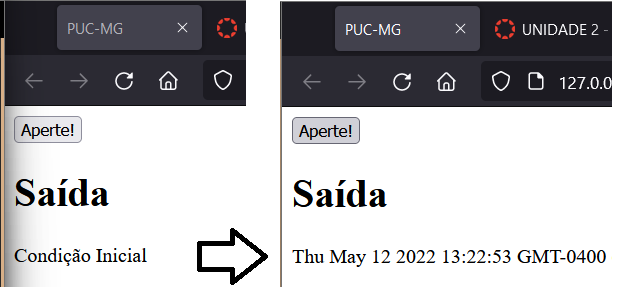
\includegraphics[scale=0.7]{21-JS-DOM-script.png}
	\caption{Manipulação do HTML com DOM e JS}
\end{figure}

\textbf{Objeto Navigator}
\\~\\
Como o próprio deixa claro, o objeto navigator representa o software do navegador usado pelo user. Esse objeto nos dá algumas informações úteis sobre o navegador usado. Abaixo temos uma tabela com alguns dos métodos contidos nesse objeto.

\begin{center}
	\begin{tabular}{|c|c|}
		\hline
		Propriedade & Descrição \\
		\hline
		\hline
		\verb|appCodeName| & Codigo do navegador \\
		\hline
		\verb|appName| & Nome do navegador \\
		\hline
		\verb|appVersion| & Versão do navegador \\
		\hline
		\verb|cookieEnabled| & Cookies habilitados \\
		\hline
		\verb|geolocation| & Geolocation \\
		\hline
		\verb|language| &  \\
		\hline
		\verb|onLine| & Se o browser está online \\
		\hline
		\verb|platform| & Qual sistema operacional \\
		\hline
		\verb|product| & Engine do navegador \\
		\hline
		\verb|userAgent| & \begin{tabular}{ll} User-agent que o browser\\envia ao navegador \end{tabular} \\
		\hline
	\end{tabular}	
\end{center}

Abaixo temos um exemplo de página web adaptado do material do curso que faz uso o objeto navegador e retorna a geolocalização do navegador.

\scriptsize
\begin{center}
\begin{Verbatim}[tabsize=4,frame=single]
<!DOCTYPE html>
<html lang="en">
<head>
    <title>PUC-MG</title>
    <script type="text/javascript">
        // funcao que recebe as coord e retorna um string
        function showPosition(position) {
            lat = position.coords.latitude
            long = position.coords.longitude
            texto = `Lat: ${lat} e Long ${long}`

            document.getElementById('saida').innerHTML = texto
        }

        // funcao que muda o HTML do elemento saida
        function getPosition() {
            if (window.navigator.geolocation) {
                window.navigator.geolocation.getCurrentPosition(showPosition)
            } else {
                x.innerHTML = 'Não tivemos acesso a' + 
                'sua localização!'
            }
        }
    </script>
</head>
<body>
    <button type="button" onclick="getPosition()">
        Geolocation
    </button>
    <h1>Mensagem</h1>
    <div id="saida">Sua localização vai aparecer aqui!</div>
</body>
</html>
\end{Verbatim}
\end{center}
\normalsize

Nesse código acima temos uma página simples com um botão que, ao ser ativado, dispara a função \verb|getPosition()|. Essa função dispara uma outra função chamada \verb|showPosition|. O resultado pode ser visto na imagem abaixo\footnote{Eu só dei uma censurada porque segurança nunca é demais.}.

\begin{figure}[H]
	\centering
	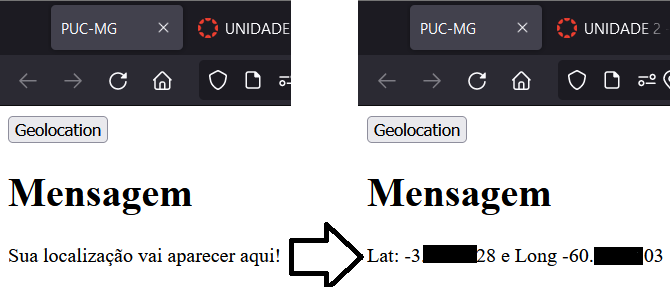
\includegraphics[scale=0.7]{22-JS-DOM-navigator.png}
	\caption{Utilização do Objeto Navegador}
\end{figure}

\textbf{Eventos}
\\~\\
Outra funcionalidade interessante do DOM é a capacidade de usarmos não apenas os elementos da página mas também o contexto (ou eventos) em que esses elementos se encontram. Por exemplo, é comum vermos uma imagem aumentar de tamanho quando colocamos o mouse sobre ela. Com essa funcionaliade, conseguimos explorar vários cenários de interação do usuário com a página.
\\~\\
No exemplo abaixo,  temos o uso de dois contextos do mouse sobre um elemento de texto. Quando o mouse está sobre o elemento, nós mudamos a cor dele para vermelho. Quando o mouse não está sobre o elemento, a cor dele se torna preto.

\begin{center}
\begin{Verbatim}[tabsize=4,frame=single]
<!DOCTYPE html>
<html lang="en">
<head>
	<title>PUC-MG</title>
</head>
<body>
	<p onmouseover="this.style.color='red'" 
		 onmouseout="this.style.color='black'">
		 
		Texto

	</p>
</body>
</html>
\end{Verbatim}
\end{center}

Podemos ver mais um exemplo do uso do token \verb|this| mas dessa vez fora de um bloco de código de uma função. Nesse contexto, esse operador faz referência ao elemento HTML e altera o seu valor do parâmetro de estilo que indicamos (a cor do texto).
\\~\\
Mesmo sendo possível fazer uso do atributo de evento direto no HTML, como fizemos no exemplo anterior, a boa prática é manter essas features em um arquivo JS à parte (igual nós fizemos com o CSS) pois isso torna o arquivo de estrutura mais fácil de ler. Abaixo temos exatamente a mesma funcionalidade mas usando o campo de script do meta mas que poderia ser hospedado em um arquivo .js em separado.

\scriptsize
\begin{center}
\begin{Verbatim}[tabsize=4,frame=single]
<!DOCTYPE html>
<html lang="en">
<head>
    <title>PUC-MG</title>
</head>
<body>
    <p id="texto">
        Texto
    </p>
</body>

<script type="text/javascript">
    var elem = window.document.getElementById('texto')

    elem.addEventListener('mouseout',
    function () {
        window.document.getElementById('texto').style.color = ''
        window.document.getElementById('texto').style.fontSize = ''
    }, false)

    elem.addEventListener('mouseover',
    function () {
        window.document.getElementById('texto').style.color = 'red'
        window.document.getElementById('texto').style.fontSize = '20px'
    }, false)
</script>
</html>
\end{Verbatim}
\end{center}
\normalsize

Veja que primeiro nós criamos uma variável \verb|elem| utilizando o \verb|getElementById|. Como essa variável é um objeto, podemos usar um de seus métodos chamado \verb|addEventListener| que recebe 3 parâmetros: o primeiro é o gatilho de disparo, o segundo é a função que será executada e o terceiro é, para todos os efeitos, sempre falso.\footnote{Você pode pesquisar um pouco se estiver curioso do motivo disso.}
\\~\\
No exemplo acima temos dois gatilhos de eventos cadastrados. O primeiro é o \verb|mouseout| que nada mais é que o padrão. O segundo é \verb|mouseover| que dispara sempre que o mouse estiver sobre o elemento selecionado.
\\~\\
Mesmo que a primeira vista pareça mais simples usar os atributos de contexto direto no HTML, nós precisamos pensar em situações onde a aplicação se torna demasiada grande. Nesses casos, é muito melhor, para controlar a evolução da nossa aplicação web e garantir uma boa manutenção, mantermos em arquivos separados tanto o estilo quanto a funcionalidade.
\\~\\
Outra coisa importante a ser notada é que o script deve estar abaixo da variável que será manipulada. Primeiro o elemento precisa existir para usarmos o nosso código. Esse é o motivo da tag \verb|script| estar na parte de baixo da página e não no \verb|head| como nos outros exemplos.
\\~\\
Na tabela a baixo temos os principais tipos de gatilhos que podem ser usados pelo DOM. Para usar algum desses no direto no HTML é necessário colocar a palavra `on' na frente. Por exemplo, `click' vira `onclick'.

\begin{center}
	\begin{tabular}{|l|l|}
	\hline
	\textbf{Propriedade} & \textbf{Descrição} \\
	\hline
	\verb|click| & Click em link ou elemento \\
	\hline
	\verb|change| & Default alterado em input texto \\
	\hline
	\verb|focus| & Foco em um elemento \\
	\hline
	\verb|blur| &  Ao tirar o foco \\
	\hline
	\verb|mouseover| & Mouse em cima  \\
	\hline
	\verb|mouseout| &  Mouse em outro lugar \\
	\hline
	\verb|select| &  Select em um form \\
	\hline
	\verb|submit| &  Submit em um form \\
	\hline
	\verb|resize| &  Mudança na janela do broser \\
	\hline
	\verb|load| & Algum elemento é carregado \\
	\hline
	\verb|unload| & Ao sair da página \\
	\hline
\end{tabular}
\end{center}

\textbf{Comentário:} Aqui o professor da disciplina faz o desafio de criarmos uma calculadora simples com o uso dos elementos estudados nessa seção. Um dia eu volto aqui e faço esse desafio.

\subsubsection{A Notação de Objetos (JSON)}

O JavaScript Object Notation (JSON) é um formato de descrição de dados que se baseia em texto e pode ser lido diretamente sem muita dificuldade. Existem vários outros tipos de escrita de dados onde, geralmente, temos um trade-off entre eficiência versus simplicidade. Quanto mais próximo da linguagem de máquina, melhor é pro computador processar mas mais difícil é para os humanos entender.
\\~\\
Como o JSON se popularizou muito, diversas outras linguagens já possuem a capacidade de processar dados nesse formato. O que aumenta ainda mais a aceitabilidade dele como veículo de envio e codificação de informação tanto no frontend quanto no backend.
\\~\\
Falando em backend, com a popularização de programas como nodejs, é cada vez mais comuns a construção de comunicação entre a camada de aplicação web e servidor através de APIs cuja atividade é, simplificadamente, receber JSON e enviar JSON.
\\~\\
Como dito anteriormente, o JSON não é o único formato existente no mercado. Para destacar alguns outros, temos o XML, RDF, Planilhas, CSV, Documentos TXT, JPEG-2000, TIFF e vários outros formatos proprietários. Mas, sem dúvida, a competição mais árdua é entre JSON e XML.
\ 
\\~\\
\textbf{Sintaxe do JSON}
\\~\\
Um arquivo JSON é muito parecido com um bloco de código JS. Começa e termina com chaves \verb|{}| e cada elemento é formado por um par de nome-valor e são separados por vírgula. O JSON permite diferentes tipos de valores que podem ser dos mesmo tipos de dados que estudamos anteriormente para o JS. Abaixo temos um exemplo de um arquivo JS.

\begin{center}
\begin{Verbatim}[tabsize=4,frame=single]
{
	"idade": 28,
	"nome": "Bruno Ruas",
	"materias": [
	{
		"materia": "Econometria",
		"professor": "Bill Gates"
	},
	{
		"materia": "Microeconomia",
		"professor": "Steve Jobs"
	}
	],
	"nerd":true
}
\end{Verbatim}
\end{center}

Nesse exemplo, podemos ver que o valor para Idade é do tipo number. Nome é uma string. Matérias é um array, veja que ele está entre colchetes \verb|[]|, exatamente como aprendemos antes. Cada elemento do nosso array de matérias é um objeto, que começam e terminam com chaves, com duas propriedades: matéria e professor. Por fim, temos um booleano para a pegunta "É nerd?".
\\~\\
Os outros tipos de dados como datas, geolocalização e outros, são passados em JSON como uma string. Temopos que lembrar disso se um dia precisamos lidar com esse tipo de informação.
\\~\\
\textbf{Comentário:} Quando estamos criando um JSON dentro de um código JS nós não precisamos colocar as aspas no nome dos elementos. Mas é padrão que essas aspas sejam usadas em objetos JSON. Então temos que ficar atentos a isso também.
\ 
\\~\\
\textbf{Objeto JSON no JavaScript}
\\~\\
Agora que sabemos um pouco sobre esse tipo de estrutura de dados, vamos aprender como manipular esse objeto dentro de um script JS. A maneira que o JS tem que trabalhar com JSON é por meio de um objeto nativo da linguagem chamado, nem um pouco sem querer, de JSON. Esse objeto possui dois métodos úteis: Um \verb|parse()| que recebe uma string e retorna um objeto na notação JSON e um \verb|stringfy()| que pega um objeto análogo JSON e transforma em string.

\begin{center}
\begin{Verbatim}[tabsize=4,frame=single]
// JSON em string
var TextoJSON = `{"Revistas": [
    {
        "titulo":"V de Vingança",
        "autor":"Frank Miller"
    },
    {
        "titulo":"Batman - The Dark Knight",
        "autor":"Frank Miller"
    },
    {
        "titulo":"One Piece Nº 29",
        "autor":"Eichiro Oda"
    }
]}`

// Usando o metodo de parse do JSON
var banca = JSON.parse(TextoJSON)

function listaTitulos() {
    lista = ''
    for (let i = 0; i < banca.Revistas.length; i++) {
        lista += banca.Revistas[i].titulo + ' - ' +
        banca.Revistas[i].autor + '\n'
    }
    console.log(lista)
}

listaTitulos()

> V de Vingança - Frank Miller
> Batman - The Dark Knight - Frank Miller
> One Piece Nº 29 - Eichiro Oda
\end{Verbatim}
\end{center}

Primeiro nós criamos uma string no formato de um JSON. Depois passamos essa string pelo objeto JSON com o método \verb|parse|. Após isso, nós temos um objeto chamado banca com a mesma estrutura do nosso JSON desejado. Depois nós criamos uma função de loop que retorna uma string com o título, o autor e o caracter especial de quebra de linha \verb|\n|.
\\~\\
Para converter nosso objeto novamente para string basta usarmos o seguinte comando:
\begin{center}
\begin{Verbatim}[tabsize=4,frame=single]
JSON.stringify(banca,null,2)
\end{Verbatim}
\end{center}

O primeiro parâmetro é o objeto a ser convertido. O segundo nós podemos colocar como null\footnote{Existe uma explicação para isso mas não precisamos dela agora.}. Por fim, o terceiro diz o tamanho do espaço para melhorar a identação.
\\~\\
Saber como lidar com objetos JSON dentro de um script JS nos permite construir aplicações inteiras apenas com JS. Um framework muito famoso hoje em dia chamado MEAN (MongoDb, Express, Angular e NodeJS) utiliza o JS como principal linguagem para construção de toda a aplicação web.

\subsubsection{Programação Ajax}

Diferente do que vimos até agora, o \textbf{Asynchronous Javascript and XML} ou AJAX, não é uma tecnologia propriamente dito mas sim uma técnica de programação que utiliza diferentes tecnologias. A ideia geral é construir ferramentas que possuam as seguintes características:
\begin{itemize}
	\item Paginas com padrão XHTML e CSS
	\item Dinâmica através do DOM
	\item Troca de informações por JSON, XML ou outro
	\item Recuperação assincrôna de dados com o objeto XMLHTTPRequest ou APT fetch
	\item JavaScript como linguagem
\end{itemize}

Algumas aplicações muito famosas foram construída usando, em algum grau, essa abordagem. Podemos citar o Youtube, Gmail, Google Earth e mais um monte de outras aplciações do Google.
\\~\\
Para entendermos como o AJAX é diferente da abordagem tradicional, vamos comparar as duas maneiras. No modelo tradicional, o browser faz requisições ao web server que, por sua vez, devolte a página solicitada com as devidas alterações previamente programadas. Contudo, nessa abordagem, toda a inteligência de negócio é mantida no ambiente do servidor. O esquema abaixo nos permite relembrar como é feita a comunicação entre essas duas entidades.

\begin{figure}[H]
	\centering
	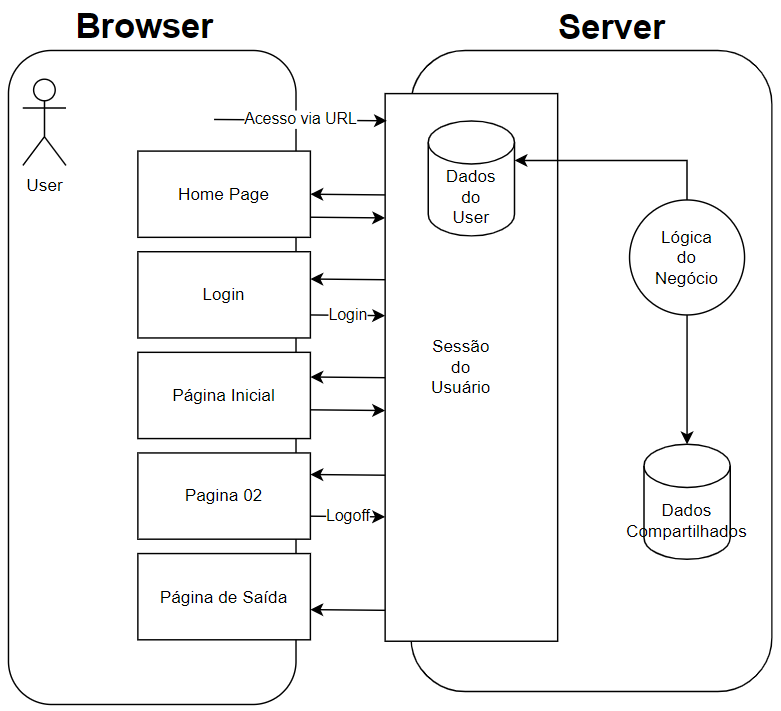
\includegraphics[scale=0.5]{23-webapp-tradicional.png}
	\caption{Esquema de uma aplicação web tradicional}
\end{figure}

O problema dessa abordagem tradicional é que os dados enviados entre servidor e browser são páginas inteiras. O método AJAX trouxe a possibiliadde de quebramos esses dados em "pacotes"\ menores de informações. Nesse caso, ao invés de requisições de páginas inteiras, podemos pedir ao servidor apenas "pedaços"\ menores de informação.
\\~\\
A metodologia AJAX trás para o lado do cliente (client side) parte da tarefa de processar os dados. Parte do processamento fica no server side e a outra parte é feita no client. Durante a sessão, várias requisições são feitas do browser (que contém o código JS) para o server por meio do uso do XMLHTTPRequest ou API Fetch. A atualização da página acontece via DOM e não pelo recebimento de um HTML novo.
\\~\\
Essa comunicação acontece geralmente por meio de arquivos XML ou JSON (mas pode ser qualquer outro formato de dados).

\begin{figure}[H]
	\centering
	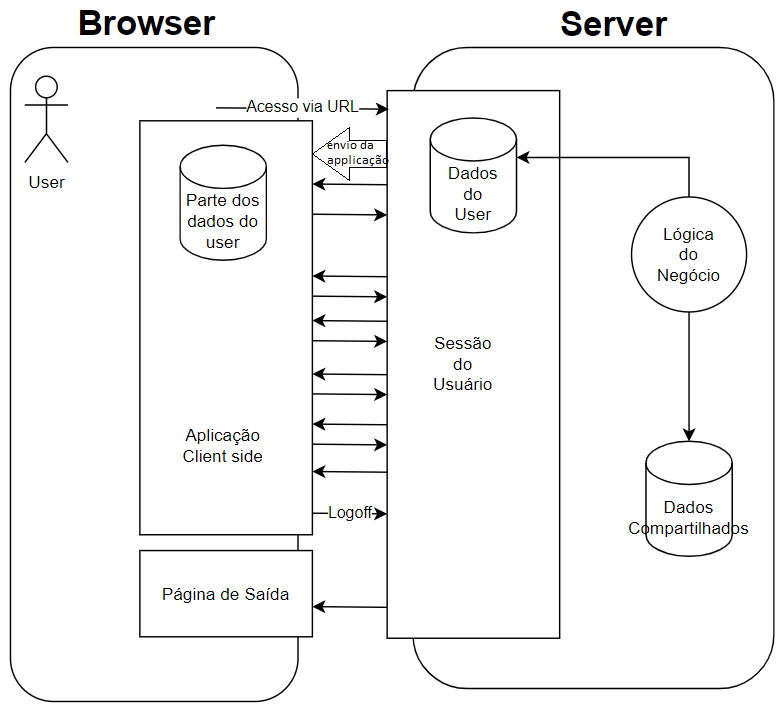
\includegraphics[scale=0.5]{24-webapp-ajax.png}
	\caption{Esquema de uma aplicação web com AJAX}
\end{figure}

Ao abrirmos a aplicação pela primeira vez, o servidor nos envia a maior parte dos dados que serão usados na visualização (a base de toda a aplicação). Depois disso, todas as mudanças na tela serão baseadas em DOM e arquivos de dados JSON ou XML.
\\~\\
Podemos elencar algumas vantagens desse modelo de construção de solução web:
\begin{itemize}
	\item Redução do tráfego na rede
	\item Redução de carga no web server
	\item Flexibilidade no desenolvimento do lado do server (foco em APIs)
\end{itemize}

Mas como tudo na vida, o AJAX possui algumas desvantagens:
\begin{itemize}
	\item Maior complexidade de desenvolvimento
	\item Aplicação mais pesada no client
	\item Só funciona em navegadores mais modernos
	\item Pode precisar de ajustes dependendo do navegador do client
	\item O usuário perde a opção de avançar e voltar no seu histórico\footnote{Isso dá pra remediar mas não é simples.}
\end{itemize}

\textbf{Objeto XMLHTTPRequest}
\\~\\
Agora que entendemos melhor o que é o AJAX e como podemos construir aplicações com ele, precisamos entender bem uma das suas principais ferramentas: o objeto XMLHTTPRequest. Inicialmente criado pelo Microsoft e adaptado pelo Mozilla, o XMLHTTPRequest é um objeto (mas também pode ser interpretado como uma API) que é fornecido pelo próprio navegador e que permite que nosso código JS troque dados com um servidor web.
\\~\\
O objeto XMLHTTPRequest é a base do AJAX. Mas cuidado. Apesar do nome, ele aceita a troca de informações em diferentes formatos além do XML: JSON, HTML, TXT, XML. Além disso por ele podemos nos conectar à serviços por outros métodos além do HTTP.
\\~\\
Para aprender como usar essa ferramenta, vamos por partes. Podemos começar o nosso script com a criação de um objeto que será do tipo XMLHTTPRequest.

\scriptsize
\begin{center}
\begin{Verbatim}[tabsize=4,frame=single]
// funcao caso a conexao funcione
function success() {
		window.document.getElementById('texto').innerHTML = this.responseText
}

// funcao caso a conexao de erro
function error(err) {console.log('Erro:',err)}


// criacao do objeto XmlHttpRequest
var xhr = new XMLHttpRequest()

// executa a funcao success se a requisicao funcionar
xhr.onload = success

// executa um funcao erro se a conexao nao funcionar
xhr.onerror = error

// defindo a requisicao
xhr.open('GET','https://api.github.com/users/brunoruas2')

xhr.send()
\end{Verbatim}
\end{center}
\normalsize

Esse script acima executa uma consulta a uma url do github que retorna um JSON com informações a respeito da conta de algum usuário. Essa requisição é feita no método \verb|send()|. Em caso de sucesso, o xhr dispara a função \verb|success| que, por sua vez, altera usa o DOM para printar na tela o JSON coletado. Em caso de erro, ele mostra, no console\footnote{Para acessar basta apertar f12 em qualquer navegador moderno.} com uma mensagem de texto que contém o erro.
\\~\\
Como podemos perceber (e como quase tudo em JS) existem vários métodos úteis no objeto XMLHttpRequest que devemos aprender. Abaixo temos uma tabela de referência com esses métodos.

\begin{center}
	\begin{tabular}{|l|l|}
	\hline
	\textbf{Propriedade} & \textbf{Descrição} \\
	\hline
	\hline
	\verb|status| & Codigo HTTP da resposta \\
	\hline
	\verb|statusText| & Texto da resposta \\
	\hline
	\verb|readyState| & Status do pedido \\
	\hline
	\verb|responseTexte| & Txt bruto da resposta \\
	\hline
	\verb|responseXML| & \begin{tabular}{l}
											 			Resposta em um objeto \\
														no DOM. Mas só funciona \\
														Se o tipo for text/xml
											 \end{tabular} \\
	\hline
	\verb|onreadystatechange| & \begin{tabular}{l}
											 			       Dispara uma função quando \\
																	 o readState muda
											        \end{tabular} \\
	\hline
	\verb|onerror| & Executa função se erro \\
	\hline
	\verb|onprogress| & \begin{tabular}{l}
											  Dispara uma função em \\
												caso de demora na resposta
											\end{tabular} \\
	\hline
	\verb|onload| & Função se o send funcionar \\
	\hline
\end{tabular}
\end{center}

Para cada requisição, o método readyState retorna um estágio diferente. Podemos pensar que cada requisição possui uma série de passos a serem feitos até a sua conclusão. Esses passos são lidos pelo método onreadystatechange e possuem características que podemos ver na lista abaixo.
\\~\\
Os estágios de uma requisição são:
\begin{itemize}
	\item \verb|Uninitialized (0)| - Objeto criado mas não iniciado
	\item \verb|Loading (1)| - Objeto criado mas não usou o método send()
	\item \verb|Loaded (2)| - Send() executado mas os cabeçalhos não estão disponíveis
	\item \verb|Interactive (3)| - Alguns dados recebidos mas não completamente
	\item \verb|Completed (4)| - Todos os dados foram recebidos e podem ser lidos
\end{itemize}

Abaixo temos um exemplo de uso do \verb|readyState| para verificação do status da chamada.

\begin{center}
\begin{Verbatim}[tabsize=4,frame=single]
function requisicaoAJAX() {
	var xmlhttp = new HMLHttpResquest()
}

xmlhttp.onreadystatechange = function() {
	if (xmlhttp.readyState == 4 && xmlhttp.status == 200) {
		divElement = document.getElementById('texto')
		divElement.innerHTML = xmlhttp.responseText
	}
}

xmlhttp.open("GET","www.google.com/api.php")
xmlhttp.send()
\end{Verbatim}
\end{center}

Podemos ver que nós criamos uma função disparada apenas quando o status muda e, como colocamos uma condição dentro, só teremos a realm modificação caso o status da comunicação seja 200 (que é o padrão para sucesso) e o status da comunicação seja o de completo.
\\~\\
\textbf{API Fetch}
\\~\\
Os navegadores atuais nos permitem uma alternativa ao XMLHttpRequest chamada API Fetch. A vantagem é que essa nova tecnologia nos permite fazer uso das \textit{promises} que simplifica a escrita da programação assíncrona. Podemos ver um exemplo abaixo.

\begin{center}
\begin{Verbatim}[tabsize=4,frame=single]
<script>
	fetch('https:api.github.com/users/brunoruas2')
		.then(res => res.json())
		.then(data => console.log(data))
		.catch(err => console.log('Erro: ', err))
</script>
\end{Verbatim}
\end{center}

\textbf{Comentário:} O material não se aprofunda no tema, então eu volto aqui para aprofundar no futuro. Aqui tem um \href{https://developer.mozilla.org/pt-BR/docs/Web/Guide/AJAX}{[link]} com um material de referência da MDN.

%%%%%%%%%%%%%%%%%%%%%%%%%%%%%%%%%%%%%%%%%%%%%%%%%%%%%%%%%%%%%%%%%%%%%%%%
\chapter{Fundamentos de Engenharia de Software}
%%%%%%%%%%%%%%%%%%%%%%%%%%%%%%%%%%%%%%%%%%%%%%%%%%%%%%%%%%%%%%%%%%%%%%%%

\section{Bibliografia}

Bibliografia Básica

\begin{itemize}
	\item PRESSMAN, Roger S.; MAXIM, Bruce R. Engenharia de software: uma abordagem profissional. 8. ed. Porto Alegre: AMGH, 2016. E-book ISBN 9788580555349. Capítulos 1, 2, 3
	\item PRIKLADNICKI, Rafael, WILLI, Renato, e MILANI, Fabiano. Métodos ágeis para desenvolvimento de software. Porto Alegre: Bookman, 2014 1 recurso online ISBN 9788582602089 Capítulos 1,2,3,8,12,13
	\item SOMMERVILLE, Ian. Engenharia de software, 10ª ed. Pearson 768 ISBN 9788543024974 Capítulos 1,2,3,4
\end{itemize}

Bibliografia Complementar

\begin{itemize}
	\item COHN, Mike; SILVA, Aldir José Coelho Corrêa da. Desenvolvimento de software com Scrum: aplicando métodos ágeis com sucesso. Porto Alegre: Bookman, 2011. E-book ISBN 9788577808199
	\item LARMAN, Craig. Utilizando UML e padrões: uma introdução á análise e ao projeto orientados a objetos e desenvolvimento iterativo. 3. ed. Porto Alegre: Bookman, 2007. E-book (695 páginas) ISBN 9788577800476
	\item PAULA FILHO, Wilson de Pádua. Engenharia de software, v. 2 projetos e processos. 4. Rio de Janeiro LTC 2019 1 recurso online ISBN 9788521636748
	\item VETORAZZO, Adriana de Souza. Engenharia de software. Porto Alegre SAGAH 2018 1 recurso online ISBN 9788595026780
	\item WAZLAWICK, Raul Sidnei. Engenharia de software conceitos e práticas. Rio de Janeiro GEN LTC 2013 1 recurso online ISBN 9788595156173
\end{itemize}

\section{Conceitos e Processos de Software}

A engenharia de software é subárea da Ciência da Computação que lida com as atividades de desenvolvimento, operação e evolução de software. Esse campo surgiu com a crise do software de 1968.

\subsection{Definições}

Agora vamos aprender os conceitos usados ao longo do trabalho de engenharia de software:
\begin{itemize}
	\item Programa - Conjunto de instruções em uma linguagem de programação.
	\item Software - Programa + Estrutura de Dados + Documentação. 
	\item Sistema - Conjunto de elementos interdependentes de Softwares, Hardware e Pessoas. Podem ser intensivos em qualquer umas dessas 3 partes.
\end{itemize}

\subsection{Modelos e Princípios de Processo de Software}

O processo de Software é um conjunto de etapas usadas para a produção de soluções de software. Podemos elencar dois conceitos importantes que compõe o processo de software:
\begin{itemize}
	\item Descrição de Processos:
		\begin{itemize}
			\item Atividades - Lista de etapas necessárias.
			\item Produtos ou Artefatos - Produto gerado pelas atividades.
			\item Papéis - Quem executa cada atividade.
			\item Condições - As requisições pré e pós execução das atividades.
		\end{itemize}
	\item Modelos de Ciclo de Vida:
		\begin{itemize}
			\item Modelo Sequencial Linear \\
				Análise/Projeto/Codificação/Teste.
			\item Modelo em Cascata \\
				Definição/Projeto/Implementação/Integração/Manutenção.
			\item Modelo Incremental \\
				O projeto é quebrado em incrementos e cada incremento possui um modelo sequencial linear ou em cascata.
			\item Modelo Incremental Evolutivo \\
				Esboço/loop{Especificação/Desenvolvimento/Validação} até que se tenha a versão final.
			\item Modelo Espiral \\
				loop{Planejamento/Modelagem/Construção/Entrega/Feedback} para cada incremento novo ao software.
			\item Modelo Iterativo \\
				É o modelo Sequencial Linear mas com possibilidade de retorno para as etapas anteriores até que se esteja aprovado pelo cliente.
			\item Modelo V \\
				Durante todas as etapas de processo de software nós já vamos definindo os testes que serão usados para a aprovação do produto. 
		\end{itemize}
\end{itemize}

Hoje em dia, temos dois modelos mais usados. A modelo incremental foca em entregar um pedaço de cada vez e o modelo iterativo permite entregar versões mais simples do produto e ir aprimorando elas. O modelo atual mais usado é justamente o \textbf{Modelo incremental iterativo}.
\\~\\
Agora que aprendemos o conceito de modelo de processo de software, vamos analisar algumas abordagens de elaboração de software. Podemos dizer que existem 3 grupos principais de processos de gestão de software: 1) Processos ágeis; 2) Processos Prescritivos e 3) Processos Enxutos (lean process).
\\~\\
\textbf{Comentário:} No material do curso só foram abordadas os dois primeiros processos.

\subsection{Processos Ágeis}

Os processos ágeis nasceram no final do século XX. Seguem o modelo incremental e iterativo de desenvolvimento. Os incrementos são pequenos e sucessivos (2 a 3 semanas). O cliente está constantemente em contato com o produto gerado no ciclo. A documentação é reduzida porque há muita comunicação interpessoal.
\\~\\
Existem várias metodologias mas podemos elencar alguns:
\begin{itemize}
	\item eXtreme Programming (XP)
	\item Scrum
	\item Dynamic System Development (DSDM)
	\item Feature Driven Development (FDD)
	\item Crystal Families
\end{itemize}

Hoje em dia o método mais usado é o Scrum. A novidade dele é que a abordagem do desenvolvimento é empírica e permite a evolução dos requisitos do processo ao longo do processo.
\\~\\
O Scrum é divido em apenas 3 etapas: 1) Planejamento inicial do projeto; 2) Loop de desenvolvimento e feedback (chamado de sprint) e 3) Entrega ao cliente.
\\~\\
As equipes do scrum são pequenas, multidisciplinares, de liderança diluída e trabalham com um foco de melhorias pequenas em um prazo mais curto (2 ou 4 semanas). Existe a figura do facilitador do processo chamado Scrum Master.
\\~\\
Os requisitos do software são mantidos no artefato chamado \textbf{Backlog} e serve de norte pada os times de desenvolvimento.
\\~\\
Existem 3 papeis no processo de gestão do Scrum:
\begin{itemize}
	\item Product Owner (PO) - O cliente ou alguém representante da vontade dele. Podemos pensar no PO como a ponte entre a empresa-cliente e a empresa-desenvolvedora.
	\item Scrum Master - É o facilitador do time de desenvolvimento. Atua como ponte entre o time de desenvolvimento e o PO. Atentemos para o fato do PO não participar do processo de desenvolvimento técnico.
	\item Equipe de Desenvolvimento - É auto-organizada e responsável pela produção dos algoritmos que comporão o software.
\end{itemize}

Agora veremos de maneira organizada os artefatos produzidos no processo de Scrum:
\begin{itemize}
	\item Backlog do Produto - Lista de características necessárias ao software atreladas a um grau de importância. Cada característica é fruto de uma \textbf{história de usuário} que é composta de 3 informações (quem?; o que? e por quê?).
	\item Backlog da Sprint - É um subconjunto das características elencadas do backlog do produto. Esses itens serão o foco da sprint (2 a 4 semanas).
	\item Incremento do Produto - É o resultado do trabalho realizado na sprint.
\end{itemize}

Além dos papéis e dos artefatos, existem as cerimônias do modelo Scrum:
\begin{itemize}
	\item Reunião de planejamento da Sprint - Decide quais características do Backlog do projeto serão objeto de trabalho pelo time de desenvolvimento.
	\item Daily - Acompanhamento a cada 24 horas do esforço do time de desenvolvimento para o alcance do planejamento da sprint. Algo rápido (15 min).
	\item Revisão da Sprint - Avaliação pelo PO do cumprimento do backlog da sprint. Foco no produto.
	\item Retrospectiva da Sprint - Melhoria do processo por meio de feedback de todas as partes envolvidas no processo de sprint. Foco no processo.
\end{itemize}

\subsection{Processos Prescritivos}

Antes do predomínio das metodologias ágeis, os processos de controle de produção de software eram orientados por processos prescritivos, também são chamados de processos dirigidos por planos. A ideia é primeiro planejar tudo e ir visualizando o caminhar dos trabalhos em termos do planejamento inicial. O Rational Unified Process (RUP) é o mais famoso desses modelos.
\\~\\
O RUP hoje pertence à IBM e possui algumas características principais:
\begin{itemize}
	\item Possui vários princípios dos quais podemos citar:
		\begin{itemize}
			\item Foco nos riscos principais
			\item Garantia do valor
			\item Permitir mudanças
			\item Definição da arquitetura da solução o mais breve possível
			\item Construção da solução em componentes
		\end{itemize}
	\item Baseado em componentes/etapas planejadas
		\begin{itemize}
			\item Disciplinas (o que deve ser feito) \\
				Requisitos/Análise/Projeto/Implementação/Teste
			\item Fases (as etapas de cumprimento das disciplinas) \\
				Concepção/Elaboração/Construção/Transição
		\end{itemize}
	\item Possui linguagem padronizada: Unified Modeling Language (UML)
	\item É dirigido por caso de uso
	\item Funciona por modelo iterativo-incremental
\end{itemize}

Os benefícios dos processos prescritivos ainda são vistos nas maiores empresas, principalmente relacionados ao uso da UML para definição de etapas necessárias em interações e processos. Abaixo temos um exemplo retirado do material do curso. Mais informações sobre a UML podem ser encontradas nesse \href{https://www.devmedia.com.br/modelagem-de-sistemas-atraves-de-uml-uma-visao-geral/27913}{[LINK]}.

\tiny
\begin{Verbatim}[tabsize=4,frame=single]
	Especificação do caso de uso Matricular em disciplinas do sistema de controle acadêmico. Fonte: A 
	especificação do caso de uso foi adaptada do livro BEZERRA, Eduardo. Princípios de análise e projeto 
	de sistemas com UML. Rio de Janeiro: Campus, 2003.

	Matricular em disciplinas 
	Sumário: O aluno usa o sistema para se matricular em disciplinas.
	Ator primário: aluno
	Ator secundário: Sistema Financeiro
	Pré-condições: o aluno está identificado pelo sistema

	Fluxo Principal:

	1- O aluno solicita a matrícula em disciplinas;
	2- O sistema apresenta a lista de disciplinas disponíveis para o semestre corrente para as quais o 
	alunos possui pré-requisitos;
	3– O aluno seleciona as disciplinas desejadas e solicita a matrícula;
	4- O sistema aloca o aluno em turmas de ofertas das disciplinas desejadas e informa ao aluno a turma 
	alocada para cada disciplina bem como o professor, os horários e dias da semana e as salas de aula;
	5- O aluno confirma as alocações feitas;
	6- O sistema realiza a matrícula e envia os dados para o Sistema Financeiro;
	7- O caso de uso termina.

	Fluxo Alternativo (4): Inclusão em lista de espera

	a) Se não há vaga ou oferta disponível para alguma disciplina selecionada pelo aluno, o sistema informa
	o fato ao aluno e fornece a opção de inserir o aluno em uma lista de espera para aquela disciplina;
	b) Se o aluno aceitar o sistema insere o aluno na lista de espera desejada e apresenta a posição do 
	aluno na lista. O caso de uso retorna ao passo 4;
	c) Se o aluno não aceitar o caso de uso prossegue a partir do passo 4.

	Fluxo de Exceção (4): Violação de regra de negócio relativa quantidade máxima de créditos 

	a) Se o aluno já atingiu a quantidade máxima de créditos em que pode se matricular por semestre, o 
	sistema informa a quantidade de disciplinas que ele pode se matricular e o caso de uso retorna ao 
	passo 2;

	Pós-Condições: O aluno foi inscrito em turmas das disciplinas selecionadas ou foi acrescentado a 
	listas de esperas das disciplinas selecionadas.
\end{Verbatim}
\normalsize

Ao final de cada fase são superados os marcos principais do RUP. Cada marco significa o maior risco relacionado àquela etapa. Na fase de concepção é o marco de objetivo de ciclo de vida. Na fase de elaboração é o marco que arquitetura do software. Na fase da construção é o marco da capacidade operacional inicial e, por fim, no marco da transição é o marco da entrega do produto.
\\~\\
Existem problemas nos métodos prescritivos, os principais são:
\begin{itemize}
	\item Forte apego à hierarquia
	\item Segmentação elevada do processo de construção
	\item Em situações críticas, acabam dando lugar a processos ágeis
\end{itemize}

\subsection{Quando usar cada Processo?}

Na vida real, podemos encontrar vários modelos misturados no dia a dia das empresas. As práticas em cada empresa são orgânicas e fortemente baseadas na cultura organização local.
\\~\\
Podemos sempre analisar os modelos como uma matriz de 2 eixos: Cascata x Iterativo e Disciplinado x Flexível. Aqui nós só analisamos os processos iterativos. Cabe a você saber se precisa de um processos mais formal como o RUP ou algo mais rápido e flexível como o SCRUM.

\subsection{Requisitos}

Podem ser divididos em 2 grupos: requisitos de cliente e requisitos do software. A primeira classe é focada nas necessidades dos usuários\footnote{Por meio das histórias de usuários ou dos casos de uso.} que utilização o sistema (é o problema a ser resolvido). A segunda categoria são as características que o produto deve ter para cumpri os requisitos dos clientes (são as ferramentas que o sistema terá para interagir com os users).
\\~\\
Os requisitos de software podem ser divididos em funcionais e não funcionais. Essa divisão será abordada de maneira mais detalhada abaixo.

\subsection{Requisitos Funcionais}

Os requisitos funcionais são as características que o software deve ter para resolver os problemas elencados como objetivos do sistema proposto. São definidos pelos stakeholders (user, clientes, especialistas e investidores). No SCRUM eles estão no backlog do projeto e no RUP está num documento específico para isso.
\\~\\
É uma lista de exposições breves das funcionalidades que o software fará e como ele se comportará em relação a alguma interação dos usuários. Atente para o fato que os requisitos funcionais são sempre relacionados a algum usuário e não à características técnicas do sistema.

\subsection{Requisitos Não Funcionais}

São as descrições das normas e padrões do produto de software. É aqui que definimos a linguagem de programação, o ambiente, os critérios de segurança, banco de dados, disponibilidade do produto, desempenho e etc.
\\~\\
Um requisito não funcional deve sempre citar um critério de aceitação quantificável. Desse modo, podemos realizar testes objetivos na hora de avaliar se o desenvolvimento da feature foi bem sucedido na iteração.
\\~\\
Podemos elencar alguns tipos de requisito não funcional:
\begin{itemize}
	\item Desempenho
	\item Disponibilidade
	\item Portabilidade
	\item Usabilidade
	\item Capacidade e Degradação
	\item Manutenibilidade
\end{itemize}

Outros requisitos não funcionais são relacionados ao processo de desenvolvimento. Como por exemplo:
\begin{itemize}
	\item Restrição da equipe desenvolvedora
	\item Qual processo de software deve ser usada
	\item Qual documentação deve ser criada
\end{itemize}

Além dessas duas classificações, podemos ter restrições relacionadas ao projeto de software:
\begin{itemize}
	\item Qual SGBD deve ser usado
	\item Plataforma de disponibilidade (web ou não)
	\item Qual linguagem de programação usada
	\item Qual o SO das plataformas
	\item Existência de sistema legado
\end{itemize}

Todos os requisitos não funcionais estarão no backlog da sprint através da aceitação do incremento pelo cliente e no RUP existe uma documentação específica para isso.


\section{Atividades e Artefatos da Engenharia de Software}

O processo de produção de software é divido em atividades com seus respectivos responsáveis e os artefatos criados a cada etapa finalizada.
\\~\\
As atividades são dividas em técnicas, gerenciais, testes e de apoio\footnote{Não focaremos nessa parte mas são as atividades de RH, administrativo e etc.}. Essas atividades são as que compõe toda a gestão da engenharia de software.

\subsection{Atividades Técnicas}

Dentro das atividades técnicas nós temos a \textbf{engenharia de requisitos}, \textbf{design/projeto de software}, \textbf{implementação/codificação}, \textbf{testes} e \textbf{aceitação do cliente}.
\\~\\
Podemos elencar as seguintes atividades técnicas necessárias ao bom processo de engenharia de requisitos:
\begin{itemize}
	\item Levantamento de Requisitos (Elicitação):
		\begin{itemize}
			\item Entrevistas
			\item Observação
			\item Leitura de documentação
		\end{itemize}
	\item Análise dos Requisitos:
		\begin{itemize}
			\item Análise das lacunas
			\item Modelagem gráfica
			\item Revisão das descrições
		\end{itemize}
	\item Especificação dos Requisitos:
		\begin{itemize}
			\item Descrição sem ambiguidades
			\item Linguagem natural, controlada ou específica
		\end{itemize}
	\item Validação dos Requisitos:
		\begin{itemize}
			\item Revisão de tudo
			\item Prototipagem
			\item Notações complexas podem dificultar entendimento do cliente
			\item Validação por parte do cliente
		\end{itemize}
\end{itemize}

Agora vamos ver as atividades de Projeto (design) de Software:
\begin{itemize}
	\item Ponderação das alternativas de soluções
	\item Escolha da solução que será implementada
	\item Detalhamento da solução escolhida (elaboração do projeto):
		\begin{itemize}
			\item Arquitetura do Software:
				Alto nível de abstração. Foco nos requisitos não funcionais. Representação das partes gerais da solução.
			\item Projeto Detalhado:
				Baixa abstração. Definição dos objetos e das interações. Foco nos requisitos funcionais. Algoritmos e estruturas de dados.
		\end{itemize}
\end{itemize}

Uma vez que temos os requisitos elencados e o projeto definido, entramos na etapa de implementação ou codificação.
\\~\\
Implementados os algoritmos, temos a etapa de testes de software para validar os requisitos e garantir que os objetivos sejam alcançados. Podem ser manuais ou automatizados.
\\~\\
Por fim, temos a aprovação do cliente no sentido de cumprimento das funcionalidades esperadas e da qualidade exigida da solução.
\\~\\
Após a aprovação, existe a etapa de manutenção de software que é composta da repetição de todas as etapas expostas acima. Cada manutenção ou aprimoramento passa pelas etapas descritas desde a análise de requisito até a aprovação.
\\~\\
\textbf{Medidas de Software}
\\~\\
São abordagens de medição e definição de metas para o cumprimento das etapas programadas para alcance dos objetivos da solução contratada.

\subsection{Atividades Gerenciais}

São as atividades que atuam no controle da complexidade da solução desenvolvida e podem ser dividas em \textbf{gestão de configuração}, \textbf{gestão de projeto}, \textbf{gestão de requisitos} e \textbf{gestão de processos} e, além dessas, possuem atividades afins como gestão da qualidade e estimativas de software.
\\~\\
A gestão de configuração ou gestão de versões é a atividade que cuida da manutenção e organização dos arquivos produzidos durante todo o processo de software. É a atividade que controla as atualizações dos programas e mantém a memória de todas as etapas anteriores.
\\~\\
A gerência de projeto de software é a atividade que controle a dinâmica de tempo, pessoas, custos envolvido no processo de desenvolvimento.
\\~\\
A gerência de requisitos é a atividade de controle das necessidades de mudança no escopo do projeto bem como controla as mudanças na mudança da necessidade do cliente a respeito da mudança de requisitos. Também atua na priorização dos requisitos para a definição dos focos de trabalho. Outra atribuição relacionada é o controle da rastreabilidade dos requisitos pois todas as etapas de elaboração devem ser relacionadas a algum requisito que pertença ao escopo solicitado pelo cliente.
\\~\\
A gestão de Processos é a atividade de definição e melhoria do processo de gestão de software de acordo com as boas práticas, dos modelos de capacitação e maturidade como (CMMI e MPS.BR).
\\~\\
A gestão da qualidade é a atividade que avalia as várias interfaces de dinâmicas que impactam no resultado final do produto de software.
\\~\\
A estimativa de software é a atividade de gerar previsões com base na história da empresa de desenvolvimento afim de melhorar a alocação dos recursos para cumprimento das etapas previstas no início do processo de planejamento.

\subsection{Testes de Software}

O objetivo dos testes é identificar os problemas da solução desenvolvida mas, como tudo na vida, existem restrições a quantidade e qualidade de testes possíveis de serem feitos uma vez que existem custos associados a essa atividade.
\\~\\
Diante das restrições impostas pela realidade e da complexidade do processo de desenvolvimento, é impossível, não importa o dimensionamento do esforço, garantir uma aplicação livre de erros. O foco dessa atividade é garantir que, ao dado nível de confiança requerido, que o software entregará as capacidades requeridas no projeto.
\\~\\
Os testes são necessários para garantir o cumprimento dos requisitos funcionais e não funcionais e podem ser divididos em dois tipos:
\begin{itemize}
	\item Testes Funcionais/Caixa Preta - Baseados no ponto de vista do usuário do software.
	\item Testes Estruturais/Caixa Branca - Ponto de vista de quem desenvolveu o software por meio de inputs e avaliação de outputs.
\end{itemize}

Uma boa maneira de realizar os testes funcionais é reproduzir as situações listadas nas histórias dos usuários.
\\~\\
Uma \textbf{Plano de Testes} é o documento que indica o conjunto de informações relacionadas ao teste realizado, tais como:
\begin{itemize}
	\item Testes de desempenho
	\item Testes funcionais da história de usuário x
	\item Teste de responsividade
	\item Teste de campos de formulários
	\item Teste de navegabilidade ou links
	\item Teste de ponta a ponta
\end{itemize}

No teste ponta a ponta passamos por todas as principais características e funcionalidades do produto que desenvolvimento para cumprimento dos requisitos.
\\~\\
Um plano de teste deve conter os casos de testes que, por sua vez, devem conter as seguintes informações:
\begin{itemize}
	\item Objetivo
	\item Valores de entrada
	\item Valores de saída esperada
	\item Valores de saída real
	\item Registro de execução (falha ou sucesso)
\end{itemize}

\subsection{Artefatos e Templates}

\subsubsection{Artefatos}

Os \textbf{artefatos} são um dos produtos que as atividades técnicas e gerencias produzem em cada ciclo de trabalho e podem ser usados nas etapas posteriores da execução do projeto. Existem vários tipos, vamos elencar alguns:
\begin{itemize}
	\item Artefatos do processo de desenvolvimento:
	\begin{itemize}
		\item Backlog do produto\footnote{Nós já sabemos o que é.}
		\item Diagramas de casos de usados
		\item Descrição de casos de uso
		\item Documento de especificação de requisitos \\
		Descreve os requisitos baseados em casos de uso ou outra forma de descrição.
	\end{itemize}
	\item Artefatos do processe de gerenciamento:
	\begin{itemize}
		\item Documento de arquitetura de software \\
		O nome já denuncia mas é importante porque contém vários diagramas do desenho da aplicação e como a solução foi construída em partes funcionais.
		\item Plano de Teste de software
		\item Casos de testes
		\item Lista de bugs
		\item Plano de projeto
		\item Matriz de rastreabilidade \\
		Mostra como os requisitos (que compõe as linhas da matriz) se relacionam com os artefatos produzidos durante o processo de produção.
	\end{itemize}
\end{itemize}

\subsubsection{Templates}

Nós já aprendemos o que são os artefatos de software e em que contexto eles são gerados, agora, vamos aprender algumas ferramentas e templates que nos auxiliam no processo de criação desses artefatos durante o processo de desenvolvimento de software.
\\~\\
\textbf{Comentário:} Essa seção é mais para consulta quando você precisar gerenciar algum projeto de desenvolvimento de software. Vou tentar manter os links atualizados mas caso algum deixe de funcionar, pode me avisar pelo \href{https://twitter.com/bruno_ruas2}{twitter}.
\\~\\
\textbf{Backlog do produto e Kanban}
\\~\\
Existem várias maneiras de organizar o cumprimento dos requisitos contidos no backlog do projeto. O kanban é um quadro onde transformamos cada item do backlog em unidades separáveis (geralmente post-its ou quadros) onde podemos mover para quadrantes de um board maior. Usualmente temos os quadrantes "A fazer", "Fazendo" e "Feito". Desse modo, podemos ver rapidamente o estado do desenvolvimento das atividades programadas para a sprint.
\\~\\
Existem várias ferramentas virtuais que podem ser usadas no processo como:
\begin{itemize}
	\item \href{https://trello.com/}{Trello}
	\item \href{https://www.pivotaltracker.com/}{PivotalTracker}
\end{itemize}

\textbf{Especificação de Requisitos de Software}
\\~\\
Existem vários templates disponíveis na internet:
\begin{itemize}
	\item \href{https://www.reqview.com/doc/iso-iec-ieee-29148-templates.html}{IEE/ISO/IEC 29148}
	\item \href{http://www.hectordufau.com.br/openup/openup/guidances/examples/use_case_spec_CD5DD9B1.html}{Esse exemplo}
	\item \href{https://www.volere.org/wp-content/uploads/2018/12/template14_ptbra.pdf}{Método Volere}
	\item \href{https://github.com/DroidFoundry/DroidMetronome/wiki/TEMPLATE-Documento-de-Especifica%C3%A7%C3%A3o-de-Objetivos-e-Requisitos-(EOR)}{PUC-MG}
\end{itemize}

\textbf{Documento de Arquitetura de Software}
\begin{itemize}
	\item \href{https://wiki.sei.cmu.edu/confluence/display/SAD/Template%3AArchitectureViewTemplate}{Architecture View Template}
	\item \href{https://wiki.sei.cmu.edu/confluence/display/SAD/Template:InterfaceTemplate}{Interface Template}
	\item \href{https://webstore.iec.ch/preview/info_isoiecieee42020%7Bed1.0%7Den.pdf}{IEE/ISO/IEC 42020}
\end{itemize}

Nesse link \href{https://www.cin.ufpe.br/~gta/rup-vc/core.base_rup/guidances/guidelines/test_case_81FD1D9F.html}{aqui} você pode ver como elaborar um caso de teste funcional a partir dos casos de uso.
\\~\\
Aqui tem um template de \href{https://pucminas.instructure.com/courses/49008/files/2889647?wrap=1}{ata de reunião}.
\\~\\
Por fim, temos um template de matriz de impacto de mudanças \href{https://pucminas.instructure.com/courses/49008/files/2889655?wrap=1}{aqui}. E uma matriz de rastreabilidade em excel \href{https://cdn.softwaretestinghelp.com/wp-content/qa/uploads/2013/10/Requirements-Traceability-matrix.xlsx}{aqui}.

\subsection{Desenhando Processos de Software}

Essa última seção é um exercício onde vamos colocar em prática todos os conceitos aprendidos até agora. Temos que saber que os conceitos aprendidos não são regras imutáveis na aplicação prática em um processo de software. Podemos combinar características de vários modelos durante o processo de execução de um planejamento sempre com foco na melhora contínua da qualidade do software.
\\~\\
Mesmo tendo muita flexibilidade sobre o processo de software, podemos elencar características que são obrigatórias em qualquer desenho:
\begin{itemize}
	\item Qual o modelo de ciclo de vida
	\item Quais as atividades que comporão o processo de software e quais a técnicas usadas ao longo delas
	\item Quais produtos ou artefatos serão gerados a cada etapa
	\item Os papéis dos agentes relacionados ao longo do processo
\end{itemize}

Nós começamos o nosso estudo de engenharia de software pelos modelos de ciclo de vida exatamente porque eles regem grande parte das atividades e artefatos produzidos durante todo o processo de software. A maturidade da empresa, dimensionamento da mão de obra, recursos disponíveis, verba do projeto, tempo de execução e outras características são importantes para definição do melhor modelo de ciclo de vida a ser adotado.
\\~\\
A nossa jornada pela engenharia de software vai ser em grande medida construir um amplo repertório de modelos de ciclo de vida, atividades e artefatos.
\\~\\
Para facilitar o complexo processo de software, existem várias ferramentas que centralizam as diferentes etapas e simplificam o processo de gestão:
\begin{itemize}
	\item Bizagi Modeler
	\item Eclipse Process Framework
\end{itemize}

%%%%%%%%%%%%%%%%%%%%%%%%%%%%%%%%%%%%%%%%%%%%%%%%%%%%%%%%%%%%%%%%%%%%%%%%
\chapter{Lógica Computacional}
%%%%%%%%%%%%%%%%%%%%%%%%%%%%%%%%%%%%%%%%%%%%%%%%%%%%%%%%%%%%%%%%%%%%%%%%

\section{Bibliografia}

Bibliografia Básica

\begin{itemize}
	\item HUNTER, David J. Fundamentos de Matemática Discreta. Rio de Janeiro: LTC, 2011
\end{itemize}

Bibliografia Complementar

\begin{itemize}
	\item ROSEN, Keneth H. Discrete Mathematics and its Applications. New York: McGraw-Hill, 2019
\end{itemize}

\section{Pensamento Lógico}
\subsection{Introdução}
\subsection{O que é Lógica?}
\subsection{Motivação}
\subsection{Definições}
\subsection{Subconjuntos}
\subsection{Operações sobre Conjuntos}
\subsection{Princípios da Lógica Proposicional}
\subsection{Conectivos Lógicos}
\subsection{Tabela Verdade e Equivalência Lógica}
\subsection{Predicados e Quantificadores}
\subsection{Ligando Variáveis}
\subsection{Negações}

\section{Pensamento Analítico}
\subsection{Provas de Teoremas}
\subsection{Regras de Inferência}
\subsection{Argumentos Válidos}
\subsection{Indução Matemática}
\subsection{Indução Forte}
\subsection{Recursão}
\subsection{Especificação de Sistemas}
\subsection{Verificação de Programas}

%%%%%%%%%%%%%%%%%%%%%%%%%%%%%%%%%%%%%%%%%%%%%%%%%%%%%%%%%%%%%%%%%%%%%%%%
\chapter{Matemática Básica}
%%%%%%%%%%%%%%%%%%%%%%%%%%%%%%%%%%%%%%%%%%%%%%%%%%%%%%%%%%%%%%%%%%%%%%%%

Como o escopo dessa matéria é super básico. Eu nem vou me dar o trabalho de resumir. Se quiserem ver um material mais completo, podem conferir na Bibliografia ou no meu \href{https://raw.githubusercontent.com/brunoruas2/Meus_Estudos/main/Matem%C3%A1tica/Book%20of%20Proof%20-%20Richard%20Hammack/book_of_proof.pdf}{Projeto Matemática}.

\section{Bibliografia}

Bibliografia Básica

\begin{itemize}
	\item GERSTING, Judith L. Fundamentos matemáticos para a ciência da computação. 7.Rio de Janeiro LTC 2016 1 recurso online ISBN 9788521633303
	\item HUNTER, David J. Fundamentos de matemática discreta. Rio de Janeiro LTC 2011 1 recurso online ISBN 9788521635246
	\item LIMA, Diana Maia de. Matemática aplicada à informática. Porto Alegre Bookman 2015 1 recurso online ISBN 9788582603178
	\item STEWART, James. Cálculo, v. 1. 8.ed. São Paulo (SP): Cengage Learning, 2017 E-book ISBN 9788522126859
\end{itemize}

Bibliografia Complementar

\begin{itemize}
	\item MENEZES, Paulo Blauth. Aprendendo matemática discreta com exercícios, v.19. Porto Alegre Bookman 2011 ISBN 9788577805105
	\item REVISTA DE INFORMÁTICA TEÓRICA E APLICADA. Porto Alegre: UFRGS, Instituto de informação, 1989. ISSN 0103-4308
	\item ROSEN, Kenneth H. Matemática discreta e suas aplicações. Porto Alegre ArtMed 2010 ISBN 9788563308399
	\item SIMÕES-PEREIRA, José Maunel dos Santos. Introdução à Matemática Combinatória. Editora InterciÊncia 338 ISBN 9788571932920
	\item ÁVILA, Geraldo; ARAÚJO, Luis Cláudio Lopes de. Cálculo: ilustrado, prático e descomplicado. Rio de Janeiro, RJ: LTC - Livros Tecnicos e Cientificos, 2012. E-book ISBN 978-85-216-2128-
	\item GUIDORIZZI, Hamilton Luiz. Um curso de cálculo, v. 1. 6. Rio de Janeiro LTC 2018 1 recurso online ISBN 9788521635574
\end{itemize}


%%%%%%%%%%%%%%%%%%%%%%%%%%%%%%%%%%%%%%%%%%%%%%%%%%%%%%%%%%%%%%%%%%%%%%%%
\chapter{Organização de Computadores}
%%%%%%%%%%%%%%%%%%%%%%%%%%%%%%%%%%%%%%%%%%%%%%%%%%%%%%%%%%%%%%%%%%%%%%%%

\section{Bibliografia}

Bibliografia Básica

\begin{itemize}
	\item STALLINGS, William. Arquitetura e organização de computadores. 10. ed. São Paulo: Pearson, c2018. E-book. ISBN 9788543020532
	\item CORRÊA, Ana Grasielle Dionísio (Org.). Organização e arquitetura de computadores. São Paulo: Pearson, 2017. E-book. ISBN 9788543020327
	\item PATTERSON, David A. Organização e projeto de computadores a interface hardware/software. Rio de Janeiro, GEN LTC 2017. 1 recurso online. ISBN 9788595152908
\end{itemize}

Bibliografia Complementar

\begin{itemize}
	\item TANENBAUM, Andrew S.; AUSTIN, Todd. Organização estruturada de computadores. 6. ed. São Paulo, SP: Pearson Education do Brasil, 2013. E-book. ISBN 9788581435398
	\item MONTEIRO, Mário A. Introdução à organização de computadores. 5. ed. Rio de Janeiro: LTC - Livros Técnicos e Científicos, c2007. E-book. ISBN 978-85-216-1973-4
\end{itemize}

\section{Fundamentos de Organização de Computadores}
\subsection{Representação de Dados e Sistemas Binário}

\subsubsection{Compreendendo o Sistema Decimal}

Os componentes eletrônicos digitais só permitem dois estados de tensão: 0 e 1. Isso implica que toda informação manipulada pelos computadores é representado em um sistema de \textbf{numeração binária}.
\\~\\
O nosso modelo de sistema numérico usual é o decimal (também chamado base 10). Ele é um sistema posicional porque o peso do dígito é dependente da posição dele no número. Por exemplo:

$$ 38_{10} = 3 \times 10^1 + 8 \times 10^0 = 30 + 8 $$
$$ 17,25_{10} = 10 \times 10^1 + 7 \times 10^0 + 2 \times 10^{-1} + 5 \times 10^{-2} $$

O subscrito indica o tipo de base usado. Uma característica dos sistemas posicionais é que o dígito mais a esquerda será o mais significativa (MSB - Most Significant Bit) e os à sua direita serão os LSB (Less Significant Bit).

\subsubsection{O Sistema Binário}

Como você já deve saber, no sistema binário temos apenas dois símbolos, entretanto, podemos representar todos os dígitos através deles só vamos precisar de mais dígitos binários (Binary Digit - BIT). Agora vamos aprender como representar números maiores que 1 em um sistema base 2.
\\~\\
O sistema binário é um sistema posicional (guarde isso na sua memória). Então a lógica é a mesma que os exemplos acima em base 10 mas com a diferença de multiplicarmos os números por $2^n$ onde $n$ é a posição do dígito. Nos número fracionais é igual ao sistema base 10, basta multiplicarmos as posições dos dígitos após a vírgula por números negativos da esquerda para direita.
\\~\\
Para converter um número base 10 em binário você precisa estar com a lista de potências de 2 na ponta da língua. Basta ir "caminhando"\ por ela até o maior valor abaixo do número desejado. Essa posição será o seu MSB = 1. Depois, basta ir calculando o quanto lhe falta para obter o número desejado. Abaixo nós representamos os mesmo números da seção de números base 10.

$$ 38_{10} =  1 \times 2^5 + 0 \times 2^4 + 0 \times 2^3 + 1 \times 2^2 + 1 \times 2^1 + 0 \times 2^0 = 100110_2 $$

$$ 17,25_{10} =  1 \times 2^5 + 0 + 0 + 0 + 1 \times 2^0 \ , \ 0 \times 2^{-1} + 1 \times 2^{-2} = 1001,01_2 $$

\subsubsection{O Sistema Hexadecimal}

O sistema hexadecimal por sua vez possui 16 símbolos (0,1,2,3,4,5,6,7,8,9,A,B,C,D,E,F) e pode ser convertido mais facilmente em binário que o sistema base 10. Assim a gente não precisa ficar trabalhando como binário (que acaba usando muitos dígitos para representar algum valor).
\\~\\
A conversão é feita pela equivalência entre cada 4 dígitos binários relacionados a cada símbolo hexadecimal de acordo com a tabela abaixo

\begin{center}
	\begin{tabular}{|c|c|}
		\hline
		Binário & Hexadecimal \\
		\hline
		0000 & 0 \\
		0001 & 1 \\
		0010 & 2 \\
		0011 & 3 \\
		0100 & 4 \\
		0101 & 5 \\
		0110 & 6 \\
		0111 & 7 \\
		1000 & 8 \\
		1001 & 9 \\
		1010 & A \\
		1011 & B \\
		1100 & C \\
		1101 & D \\
		1110 & E \\
		1111 & F \\
		\hline
	\end{tabular}	
\end{center}

Por exemplo, vamos converter um número hexadecimal em binário. Usando a tabela acima, podemos pegar cada dígito (1,7,F) e substituir pelo seu valor binário. Após isso, podemos descartar os zeros a esquerda do MSB.

$$ 17F_{16} =  \underset{\textrm{1}}{0001}\ \underset{7}{0111} \ \underset{F}{1111} = 10111111_2$$

Para converter de binário para hexadecimal é só começar da direita para a esquerda em cada grupo de 4 bits.

\subsection{Conceitos de Lógica Digital}

Computadores são formados por componentes eletrônicos. Os transistores e os diodos são usados para a construção das portas lógicas que nos permitem, através de circuitos elétricos, replicar os operadores lógicos da lógica usados na algebra booleana. Assumindo valores em dois estágios: 0 (de 0 a 0,6 volts) e 1 (entre 3,6 e 5 volts).
\\~\\
Uma porta lógica nada mais é que um circuito que recebe sinais de entrada e, conforme a sua configuração, produz um sinal de saída cujo valor é dependente da entrada.
\\~\\
Podemos categorizar as portas lógicas em 3 grupos:

\begin{itemize}
	\item Portas Lógicas Básicas
		\begin{itemize}
			\item Operação Lógica - AND
			\item Operação Lógica - OR
			\item Operação Inversora - NOT
		\end{itemize}
	\item Funções e Portas Lógicas Compostas
		\begin{itemize}
			\item Operação Lógica - NAND (NOT-AND)
			\item Operação Lógica - NOR (NOT-OR)
			\item Operação Lógica - XOR (OR-EXCLUSIVA)
		\end{itemize}
	\item Expressões Lógicas e Circuitos Digitais
\end{itemize}

Eu já trabalhei bem a fundo a lógica matemática no meu curso do Projeto Matemática. Você pode conferir no capítulo 02 nesse \href{https://github.com/brunoruas2/Meus_Estudos/blob/main/Matem%C3%A1tica/Book%20of%20Proof%20-%20Richard%20Hammack/book_of_proof.pdf}{[LINK]}. A única diferença é que quando lá for TRUE ou VERDADE, aqui será 1 e, claramente, quando lá for FALSE ou FALSO, aqui será 0. 
\\~\\
Como nosso estudo nesse manual é mais focado em ADS eu só vou manter as anotações referentes à transposição da algebra booleana para os circuitos eletrônicos.

\subsubsection{Operadores Básicos}

\begin{figure}[H]
	\centering
	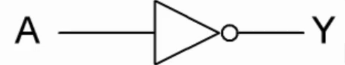
\includegraphics[scale=0.5]{01-porta_NOT.png}
	\caption{Porta NOT | Equação $Y = \overline{A}$}
\end{figure}

\begin{figure}[H]
	\centering
	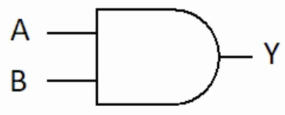
\includegraphics[scale=0.5]{02-porta_AND.png}
	\caption{Porta AND | Equação $Y = A\ . \ B $}
\end{figure}

\begin{figure}[H]
	\centering
	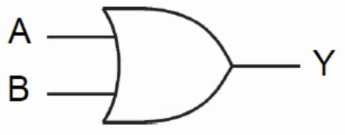
\includegraphics[scale=0.5]{03-porta_OR.png}
	\caption{Porta OR  | Equação $Y = A + B $}
\end{figure}

\subsubsection{Operadores Compostos}

\begin{figure}[H]
	\centering
	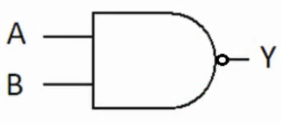
\includegraphics[scale=0.5]{04-porta_NAND.png}
	\caption{Porta OR  | Equação $Y = \overline{A\ . \ B} $}
\end{figure}

\begin{figure}[H]
	\centering
	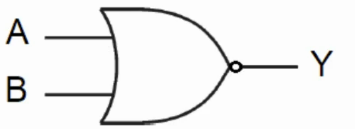
\includegraphics[scale=0.5]{05-porta_NOR.png}
	\caption{Porta OR  | Equação $Y = \overline{A + B} $}
\end{figure}

\begin{figure}[H]
	\centering
	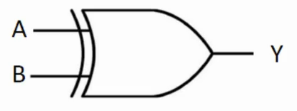
\includegraphics[scale=0.5]{06-porta_XOR.png}
	\caption{Porta OR  | Equação $Y = A \oplus B $}
\end{figure}

\subsubsection{Expressões Lógicas e Circuitos}

Podemos usar os operadores lógicos para criar expressões do tipo $ Y = (A+B).C $ que pode ser lida como "Y é igual a A ou B e C"\footnote{Usando os símbolos lógicos mais clássicos, podemos escrever como $Y: (A \lor B) \land C $}. Podemos também usar os diagramas de circuitos para representar exatamente essa mesma opração lógica.

\begin{figure}[H]
	\centering
	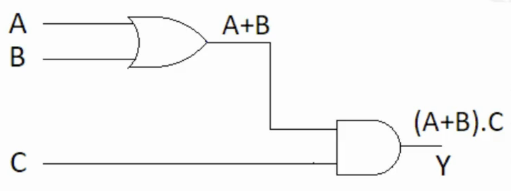
\includegraphics[scale=0.8]{07-operacao_logica.png}
\end{figure}


\subsection{Circuitos Lógicos Digitais Básicos}
\subsection{Introdução à Organização de Computadores}
\subsection{Unidade Central de Processamento - UCP}
\subsection{Memória}
\subsection{Entrada e Saída}

\section{Arquitetura de Computadores}
\subsection{Arquiteturas RISC e CISC}
\subsection{Arquitetura do Conjunto de Instruções: Exemplo do MIPS}
\subsection{Linguagem de Montagem}
\subsection{Conceito de Pipeline de Instruções}
\subsection{Paralelismo em Nível de Instruções}
\subsection{Paralelismo em Nível de Processadores}

%%%%%%%%%%%%%%%%%%%%%%%%%%%%%%%%%%%%%%%%%%%%%%%%%%%%%%%%%%%%%%%%%%%%%%%%
\chapter{Pensamento Computacional}
%%%%%%%%%%%%%%%%%%%%%%%%%%%%%%%%%%%%%%%%%%%%%%%%%%%%%%%%%%%%%%%%%%%%%%%%

\section{Bibliografia}

Bibliografia Básica

\begin{itemize}
	\item BEECHER, Karl. Computational Thinking - A beginner's guide to problem-solving and programming. Swindon, UK: BCS Learning \& Development Limited, 2017. (O´Reilly) EPUB ISBN-13: 978-1-78017-36-65
	\item FORBELLONE, André Luiz Villar; EBERSPACHER, Henri Frederico. Lógica de programação: a construção de algoritmos e estruturas de dados. 3. ed. São Paulo: Prentice Hall, 2005. xii, 218 p. ISBN 8576050242
	\item MANZANO, José Augusto N. G; OLIVEIRA, Jayr Figueiredo de. Algoritmos: lógica para desenvolvimento de programação de computadores. 28. ed. rev. e atual. São Paulo, SP: Érica, 2016. ISBN 9788536518657
\end{itemize}

Bibliografia Complementar

\begin{itemize}
	\item GUEDES, Sérgio (Org). Lógica de programação algorítmica. São Paulo: Pearson, 2014. ISBN 9788543005546
	\item MANZANO, José Augusto N. G. Estudo dirigido de algoritmos. 15. São Paulo Erica 2011 1 recurso online ISBN 9788536519067
	\item SOUZA, Marcos Fernando Ferreira de. Computadores e sociedade: da filosofia às linguagens de programação. Editora Intersaberes 208 ISBN 9788559722116
	\item TORRES, Fernando E. et al. Pensamento computacional. Porto Alegre: SAGAH, 2019. ISBN 978-85-9502-997-2
	\item FORBELLONE, André Luiz Villar; EBERSPACHER, Henri Frederico. Lógica de programação: a construção de algoritmos e estruturas de dados. 3. ed. São Paulo: Prentice Hall, 2005. xii, 218 p. ISBN 8576050242
\end{itemize}

\section{Conceitos e Competências de Pensamento Computacional}

Existem divergências quanto ao significado preciso desse conceito, contudo, as interpretações vigentes costumam convergir para a definição que o pensamento computacional é a maneira de organizar o raciocínio de modo a pensar de maneira organizada, lógica e propor soluções úteis para os problemas propostos.
\\~\\
Podemos elencar alguns pilares que fundamentam o processo de pensamento computacional:
\begin{itemize}
	\item Abstração - Construção de um modelo simplificado da questão.
	\item Decomposição - Separação do problema em diferentes partes.
	\item Reconhecimento de Padrões - Identificação de processos que se repetem.
	\item Automação (aka Algoritmo) - Construção de um processo de solução do problema.
\end{itemize}

Além desses passos, podemos acrescentar mais algumas etapas ao esforço de solução de problemas:
\begin{itemize}
	\item Paralelização - Etapas paralelas e independentes.
		\begin{itemize}
			\item Particionamento de Dados - Quebra de um grande volume de dados para processamento paralelo e posterior união do resultado.
			\item Particionamento de Tarefas - Quebra do processo em diferentes unidades executoras paralelas.
		\end{itemize}
	\item Simulação - Simplificação do caso real para melhor compreender o problema.
	\item Avaliação de Soluções - Análise dos impactos das soluções propostas.
\end{itemize}

É importante é saber que pensamento computacional não é pensar como um computador e sim de maneira organizada.
\\~\\
Esses passos não são necessariamente seguidos nessa ordem\footnote{Embora, na minha opinião, faz todo sentido seguir nessas etapas mesmo.}. Podemos pensar nessa lista como etapas necessárias mas não sucessivas. Agora veremos um pouco mais sobre cada uma delas.

\section{Computação Desplugada}

O foco dessa seção é elencar algum problemas que podem ser resolvidos com algoritmos que foram construídos usando o uso das etapadas aprendidas na seção anterior.
\\~\\
Várias situações que nós encontramos no processo de construção de uma solução podem ser entendidas como análogas a algum dos problemas elencados aqui. Por isso é bom manter anotações sempre que aprendermos uma técnica de resolução nova para um problema.

\begin{itemize}
	\item Compresão de Texto: \\
		 Resolvido com a substituição de seções longas por caracteres menores antes da transmissão. Depois enviamos as regras de codificação para processamento da mensagem original. Tópico teórico: Teoria da Informação; Codificação.
	\item Adivinhação de um Número: \\
		Basta ir perguntando pela metade das opções. Essa é a solução de menor rodadas. Tópico teórico: Árvore de Decisão; Eficiência de Algoritmos.
	\item Problema do Caixeiro Viajante: \\
		Construção de um grafo e escolha do caminho de menor soma entre as distâncias dos nós. Tópico teórico: Teoria dos Grafos.
	\item Nonograma: \\
		Procurar as regras de construção das imagens para cada linha até que se tenha um conjunto de regras para ser aplicadas nas instruções iniciais. Desafio difícil de implementar por linguagem de programação. Tópicos teóricos: Abstração; Modelagem.
\end{itemize}

%%%%%%%%%%%%%%%%%%%%%%%%%%%%%%%%%%%%%%%%%%%%%%%%%%%%%%%%%%%%%%%%%%%%%%%%
\part{Análise e Projeto de Software}
%%%%%%%%%%%%%%%%%%%%%%%%%%%%%%%%%%%%%%%%%%%%%%%%%%%%%%%%%%%%%%%%%%%%%%%%

%%%%%%%%%%%%%%%%%%%%%%%%%%%%%%%%%%%%%%%%%%%%%%%%%%%%%%%%%%%%%%%%%%%%%%%%
\chapter{Projeto: Desenvolvimento de uma Aplicação Interativa}
%%%%%%%%%%%%%%%%%%%%%%%%%%%%%%%%%%%%%%%%%%%%%%%%%%%%%%%%%%%%%%%%%%%%%%%%

%%%%%%%%%%%%%%%%%%%%%%%%%%%%%%%%%%%%%%%%%%%%%%%%%%%%%%%%%%%%%%%%%%%%%%%%
\chapter{Algoritmos e Estrutura de Dados}
%%%%%%%%%%%%%%%%%%%%%%%%%%%%%%%%%%%%%%%%%%%%%%%%%%%%%%%%%%%%%%%%%%%%%%%%

%%%%%%%%%%%%%%%%%%%%%%%%%%%%%%%%%%%%%%%%%%%%%%%%%%%%%%%%%%%%%%%%%%%%%%%%
\chapter{Desenvolvimento Web Back-End}
%%%%%%%%%%%%%%%%%%%%%%%%%%%%%%%%%%%%%%%%%%%%%%%%%%%%%%%%%%%%%%%%%%%%%%%%

%%%%%%%%%%%%%%%%%%%%%%%%%%%%%%%%%%%%%%%%%%%%%%%%%%%%%%%%%%%%%%%%%%%%%%%%
\chapter{Design de Interação}
%%%%%%%%%%%%%%%%%%%%%%%%%%%%%%%%%%%%%%%%%%%%%%%%%%%%%%%%%%%%%%%%%%%%%%%%

%%%%%%%%%%%%%%%%%%%%%%%%%%%%%%%%%%%%%%%%%%%%%%%%%%%%%%%%%%%%%%%%%%%%%%%%
\chapter{Engenharia de Requisitos de Software}
%%%%%%%%%%%%%%%%%%%%%%%%%%%%%%%%%%%%%%%%%%%%%%%%%%%%%%%%%%%%%%%%%%%%%%%%

%%%%%%%%%%%%%%%%%%%%%%%%%%%%%%%%%%%%%%%%%%%%%%%%%%%%%%%%%%%%%%%%%%%%%%%%
\chapter{Fundamentos de Redes de Computadores}
%%%%%%%%%%%%%%%%%%%%%%%%%%%%%%%%%%%%%%%%%%%%%%%%%%%%%%%%%%%%%%%%%%%%%%%%

%%%%%%%%%%%%%%%%%%%%%%%%%%%%%%%%%%%%%%%%%%%%%%%%%%%%%%%%%%%%%%%%%%%%%%%%
\chapter{Manipulação de Dados com SQL}
%%%%%%%%%%%%%%%%%%%%%%%%%%%%%%%%%%%%%%%%%%%%%%%%%%%%%%%%%%%%%%%%%%%%%%%%

%%%%%%%%%%%%%%%%%%%%%%%%%%%%%%%%%%%%%%%%%%%%%%%%%%%%%%%%%%%%%%%%%%%%%%%%
\chapter{Modelagem de Dados}
%%%%%%%%%%%%%%%%%%%%%%%%%%%%%%%%%%%%%%%%%%%%%%%%%%%%%%%%%%%%%%%%%%%%%%%%

%%%%%%%%%%%%%%%%%%%%%%%%%%%%%%%%%%%%%%%%%%%%%%%%%%%%%%%%%%%%%%%%%%%%%%%%
\chapter{Programação Modular}
%%%%%%%%%%%%%%%%%%%%%%%%%%%%%%%%%%%%%%%%%%%%%%%%%%%%%%%%%%%%%%%%%%%%%%%%

%%%%%%%%%%%%%%%%%%%%%%%%%%%%%%%%%%%%%%%%%%%%%%%%%%%%%%%%%%%%%%%%%%%%%%%%
\part{Processo de Negócio e Desenvolvimento de Software}
%%%%%%%%%%%%%%%%%%%%%%%%%%%%%%%%%%%%%%%%%%%%%%%%%%%%%%%%%%%%%%%%%%%%%%%%

%%%%%%%%%%%%%%%%%%%%%%%%%%%%%%%%%%%%%%%%%%%%%%%%%%%%%%%%%%%%%%%%%%%%%%%%
\chapter{Projeto: Desenvolvimento de uma Aplicação Móvel em um Ambiente de Negócio}
%%%%%%%%%%%%%%%%%%%%%%%%%%%%%%%%%%%%%%%%%%%%%%%%%%%%%%%%%%%%%%%%%%%%%%%%

%%%%%%%%%%%%%%%%%%%%%%%%%%%%%%%%%%%%%%%%%%%%%%%%%%%%%%%%%%%%%%%%%%%%%%%%
\chapter{Desenvolvimento de Aplicações Móveis}
%%%%%%%%%%%%%%%%%%%%%%%%%%%%%%%%%%%%%%%%%%%%%%%%%%%%%%%%%%%%%%%%%%%%%%%%

%%%%%%%%%%%%%%%%%%%%%%%%%%%%%%%%%%%%%%%%%%%%%%%%%%%%%%%%%%%%%%%%%%%%%%%%
\chapter{Estatística Descritiva}
%%%%%%%%%%%%%%%%%%%%%%%%%%%%%%%%%%%%%%%%%%%%%%%%%%%%%%%%%%%%%%%%%%%%%%%%

%%%%%%%%%%%%%%%%%%%%%%%%%%%%%%%%%%%%%%%%%%%%%%%%%%%%%%%%%%%%%%%%%%%%%%%%
\chapter{Gerência de Configuração}
%%%%%%%%%%%%%%%%%%%%%%%%%%%%%%%%%%%%%%%%%%%%%%%%%%%%%%%%%%%%%%%%%%%%%%%%

%%%%%%%%%%%%%%%%%%%%%%%%%%%%%%%%%%%%%%%%%%%%%%%%%%%%%%%%%%%%%%%%%%%%%%%%
\chapter{Gerência de Projetos de TI}
%%%%%%%%%%%%%%%%%%%%%%%%%%%%%%%%%%%%%%%%%%%%%%%%%%%%%%%%%%%%%%%%%%%%%%%%

%%%%%%%%%%%%%%%%%%%%%%%%%%%%%%%%%%%%%%%%%%%%%%%%%%%%%%%%%%%%%%%%%%%%%%%%
\chapter{Gerência de Requisitos de Software}
%%%%%%%%%%%%%%%%%%%%%%%%%%%%%%%%%%%%%%%%%%%%%%%%%%%%%%%%%%%%%%%%%%%%%%%%

%%%%%%%%%%%%%%%%%%%%%%%%%%%%%%%%%%%%%%%%%%%%%%%%%%%%%%%%%%%%%%%%%%%%%%%%
\chapter{Qualidade de Processos de Software}
%%%%%%%%%%%%%%%%%%%%%%%%%%%%%%%%%%%%%%%%%%%%%%%%%%%%%%%%%%%%%%%%%%%%%%%%

%%%%%%%%%%%%%%%%%%%%%%%%%%%%%%%%%%%%%%%%%%%%%%%%%%%%%%%%%%%%%%%%%%%%%%%%
\part{Infraestrutura para Sistemas de Software}
%%%%%%%%%%%%%%%%%%%%%%%%%%%%%%%%%%%%%%%%%%%%%%%%%%%%%%%%%%%%%%%%%%%%%%%%

%%%%%%%%%%%%%%%%%%%%%%%%%%%%%%%%%%%%%%%%%%%%%%%%%%%%%%%%%%%%%%%%%%%%%%%%
\chapter{Projeto: Desenvolvimento de um Aplicação Distribuída}
%%%%%%%%%%%%%%%%%%%%%%%%%%%%%%%%%%%%%%%%%%%%%%%%%%%%%%%%%%%%%%%%%%%%%%%%

%%%%%%%%%%%%%%%%%%%%%%%%%%%%%%%%%%%%%%%%%%%%%%%%%%%%%%%%%%%%%%%%%%%%%%%%
\chapter{APIs e Web Services}
%%%%%%%%%%%%%%%%%%%%%%%%%%%%%%%%%%%%%%%%%%%%%%%%%%%%%%%%%%%%%%%%%%%%%%%%

%%%%%%%%%%%%%%%%%%%%%%%%%%%%%%%%%%%%%%%%%%%%%%%%%%%%%%%%%%%%%%%%%%%%%%%%
\chapter{Arquitetura de Software Distribuído}
%%%%%%%%%%%%%%%%%%%%%%%%%%%%%%%%%%%%%%%%%%%%%%%%%%%%%%%%%%%%%%%%%%%%%%%%

%%%%%%%%%%%%%%%%%%%%%%%%%%%%%%%%%%%%%%%%%%%%%%%%%%%%%%%%%%%%%%%%%%%%%%%%
\chapter{Banco de Dados NoSQL}
%%%%%%%%%%%%%%%%%%%%%%%%%%%%%%%%%%%%%%%%%%%%%%%%%%%%%%%%%%%%%%%%%%%%%%%%

%%%%%%%%%%%%%%%%%%%%%%%%%%%%%%%%%%%%%%%%%%%%%%%%%%%%%%%%%%%%%%%%%%%%%%%%
\chapter{Cloud Computing}
%%%%%%%%%%%%%%%%%%%%%%%%%%%%%%%%%%%%%%%%%%%%%%%%%%%%%%%%%%%%%%%%%%%%%%%%

%%%%%%%%%%%%%%%%%%%%%%%%%%%%%%%%%%%%%%%%%%%%%%%%%%%%%%%%%%%%%%%%%%%%%%%%
\chapter{Projeto de Software}
%%%%%%%%%%%%%%%%%%%%%%%%%%%%%%%%%%%%%%%%%%%%%%%%%%%%%%%%%%%%%%%%%%%%%%%%

%%%%%%%%%%%%%%%%%%%%%%%%%%%%%%%%%%%%%%%%%%%%%%%%%%%%%%%%%%%%%%%%%%%%%%%%
\chapter{Teste de Software}
%%%%%%%%%%%%%%%%%%%%%%%%%%%%%%%%%%%%%%%%%%%%%%%%%%%%%%%%%%%%%%%%%%%%%%%%

%%%%%%%%%%%%%%%%%%%%%%%%%%%%%%%%%%%%%%%%%%%%%%%%%%%%%%%%%%%%%%%%%%%%%%%%
\part{Empreendedorismo e Inovação com Sistemas de Software}
%%%%%%%%%%%%%%%%%%%%%%%%%%%%%%%%%%%%%%%%%%%%%%%%%%%%%%%%%%%%%%%%%%%%%%%%

%%%%%%%%%%%%%%%%%%%%%%%%%%%%%%%%%%%%%%%%%%%%%%%%%%%%%%%%%%%%%%%%%%%%%%%%
\chapter{Projeto: Desenvolvimento de um Sistema Sociotecnológico Inovador}
%%%%%%%%%%%%%%%%%%%%%%%%%%%%%%%%%%%%%%%%%%%%%%%%%%%%%%%%%%%%%%%%%%%%%%%%

%%%%%%%%%%%%%%%%%%%%%%%%%%%%%%%%%%%%%%%%%%%%%%%%%%%%%%%%%%%%%%%%%%%%%%%%
\chapter{Complience em TI}
%%%%%%%%%%%%%%%%%%%%%%%%%%%%%%%%%%%%%%%%%%%%%%%%%%%%%%%%%%%%%%%%%%%%%%%%

%%%%%%%%%%%%%%%%%%%%%%%%%%%%%%%%%%%%%%%%%%%%%%%%%%%%%%%%%%%%%%%%%%%%%%%%
\chapter{Computadores e Sociedade}
%%%%%%%%%%%%%%%%%%%%%%%%%%%%%%%%%%%%%%%%%%%%%%%%%%%%%%%%%%%%%%%%%%%%%%%%

%%%%%%%%%%%%%%%%%%%%%%%%%%%%%%%%%%%%%%%%%%%%%%%%%%%%%%%%%%%%%%%%%%%%%%%%
\chapter{Empreendedorismo e Inovação}
%%%%%%%%%%%%%%%%%%%%%%%%%%%%%%%%%%%%%%%%%%%%%%%%%%%%%%%%%%%%%%%%%%%%%%%%

%%%%%%%%%%%%%%%%%%%%%%%%%%%%%%%%%%%%%%%%%%%%%%%%%%%%%%%%%%%%%%%%%%%%%%%%
\chapter{Implantação de Soluções de TI}
%%%%%%%%%%%%%%%%%%%%%%%%%%%%%%%%%%%%%%%%%%%%%%%%%%%%%%%%%%%%%%%%%%%%%%%%

%%%%%%%%%%%%%%%%%%%%%%%%%%%%%%%%%%%%%%%%%%%%%%%%%%%%%%%%%%%%%%%%%%%%%%%%
\chapter{Segurança Aplicada ao Desenvolvimento de Software}
%%%%%%%%%%%%%%%%%%%%%%%%%%%%%%%%%%%%%%%%%%%%%%%%%%%%%%%%%%%%%%%%%%%%%%%%

\end{document}
